% Created 2020-08-22 sáb 18:37
% Intended LaTeX compiler: pdflatex
\documentclass[11pt]{article}
\usepackage[utf8]{inputenc}
\usepackage{lmodern}
\usepackage[T1]{fontenc}
\usepackage[top=2cm, bottom=2cm, left=2cm, right=2cm]{geometry}
\usepackage{graphicx}
\usepackage{longtable}
\usepackage{float}
\usepackage{wrapfig}
\usepackage{rotating}
\usepackage[normalem]{ulem}
\usepackage{amsmath}
\usepackage{textcomp}
\usepackage{marvosym}
\usepackage{wasysym}
\usepackage{amssymb}
\usepackage{amsmath}
\usepackage[theorems, skins]{tcolorbox}
\usepackage[style=abnt,noslsn,extrayear,uniquename=init,giveninits,justify,sccite,
scbib,repeattitles,doi=false,isbn=false,url=false,maxcitenames=2,
natbib=true,backend=biber]{biblatex}
\usepackage{url}
\usepackage[linktocpage,pdfstartview=FitH,colorlinks,
linkcolor=blue,anchorcolor=blue,
citecolor=blue,filecolor=blue,menucolor=blue,urlcolor=blue]{hyperref}
\usepackage{attachfile}
\usepackage{setspace}
\usepackage{tikz}
\author{Pedro Paulo Zahluth Bastos, Luiz Celso Gomes Jr, Lorena Salces Dourado, Gabriel Petrini, Paulo Robilloti, Antonio Ibarra}
\date{September 2020}
\title{Impactos econômicos da COVID-19}
\begin{document}

\maketitle
\tableofcontents


\section{Dados Granulares}
\label{sec:org8e5023e}

\subsection{Energia}
\label{sec:org5a00f4b}



\subsubsection{Brazil: BRA}
\label{sec:org73f3c39}
\begin{enumerate}
\item Energy share
\label{sec:org2515006}

\begin{verbatim}
<Figure size 2400x1500 with 1 Axes>
\end{verbatim}


\begin{center}
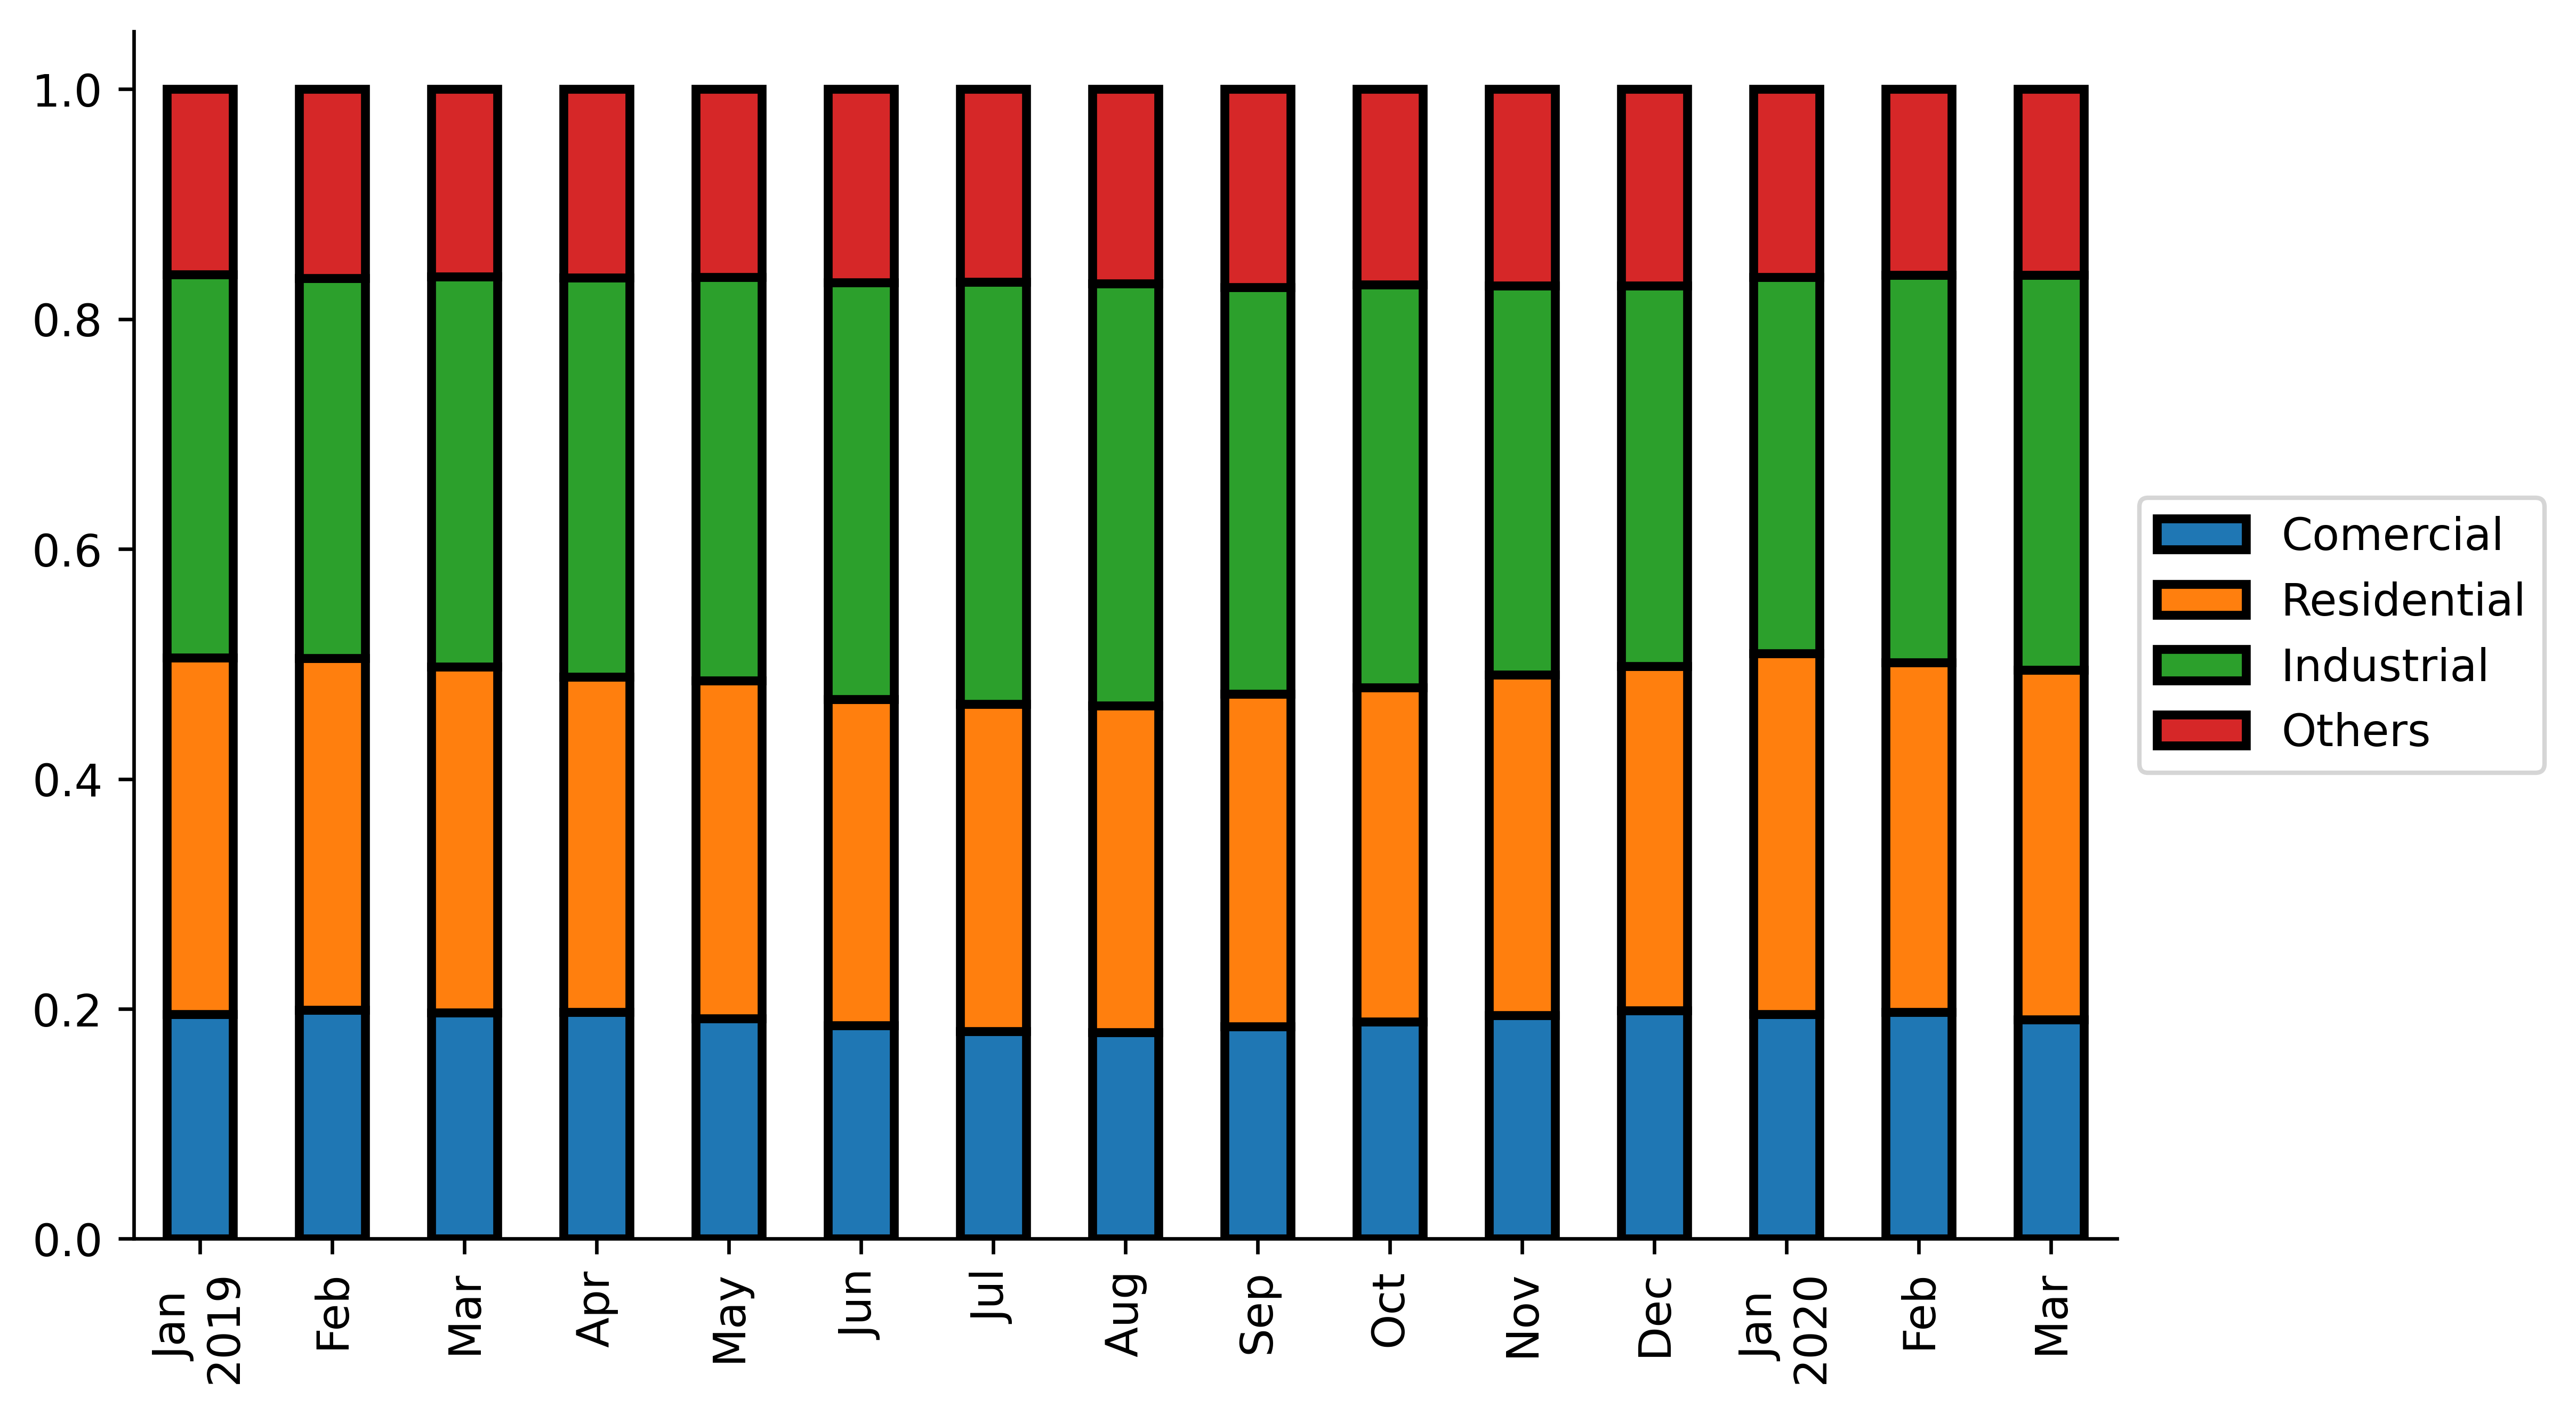
\includegraphics[width=.9\linewidth]{obipy-resources/62e383af79e91b63c7fc98dd7fb55b3c3ececcb9/b9bb93431770d5b32665b50dc4549f5f948c88a6.png}
\end{center}

\item Consumo Diário
\label{sec:orgef38e03}

\begin{verbatim}
<Figure size 2400x1500 with 2 Axes>
\end{verbatim}


\begin{center}
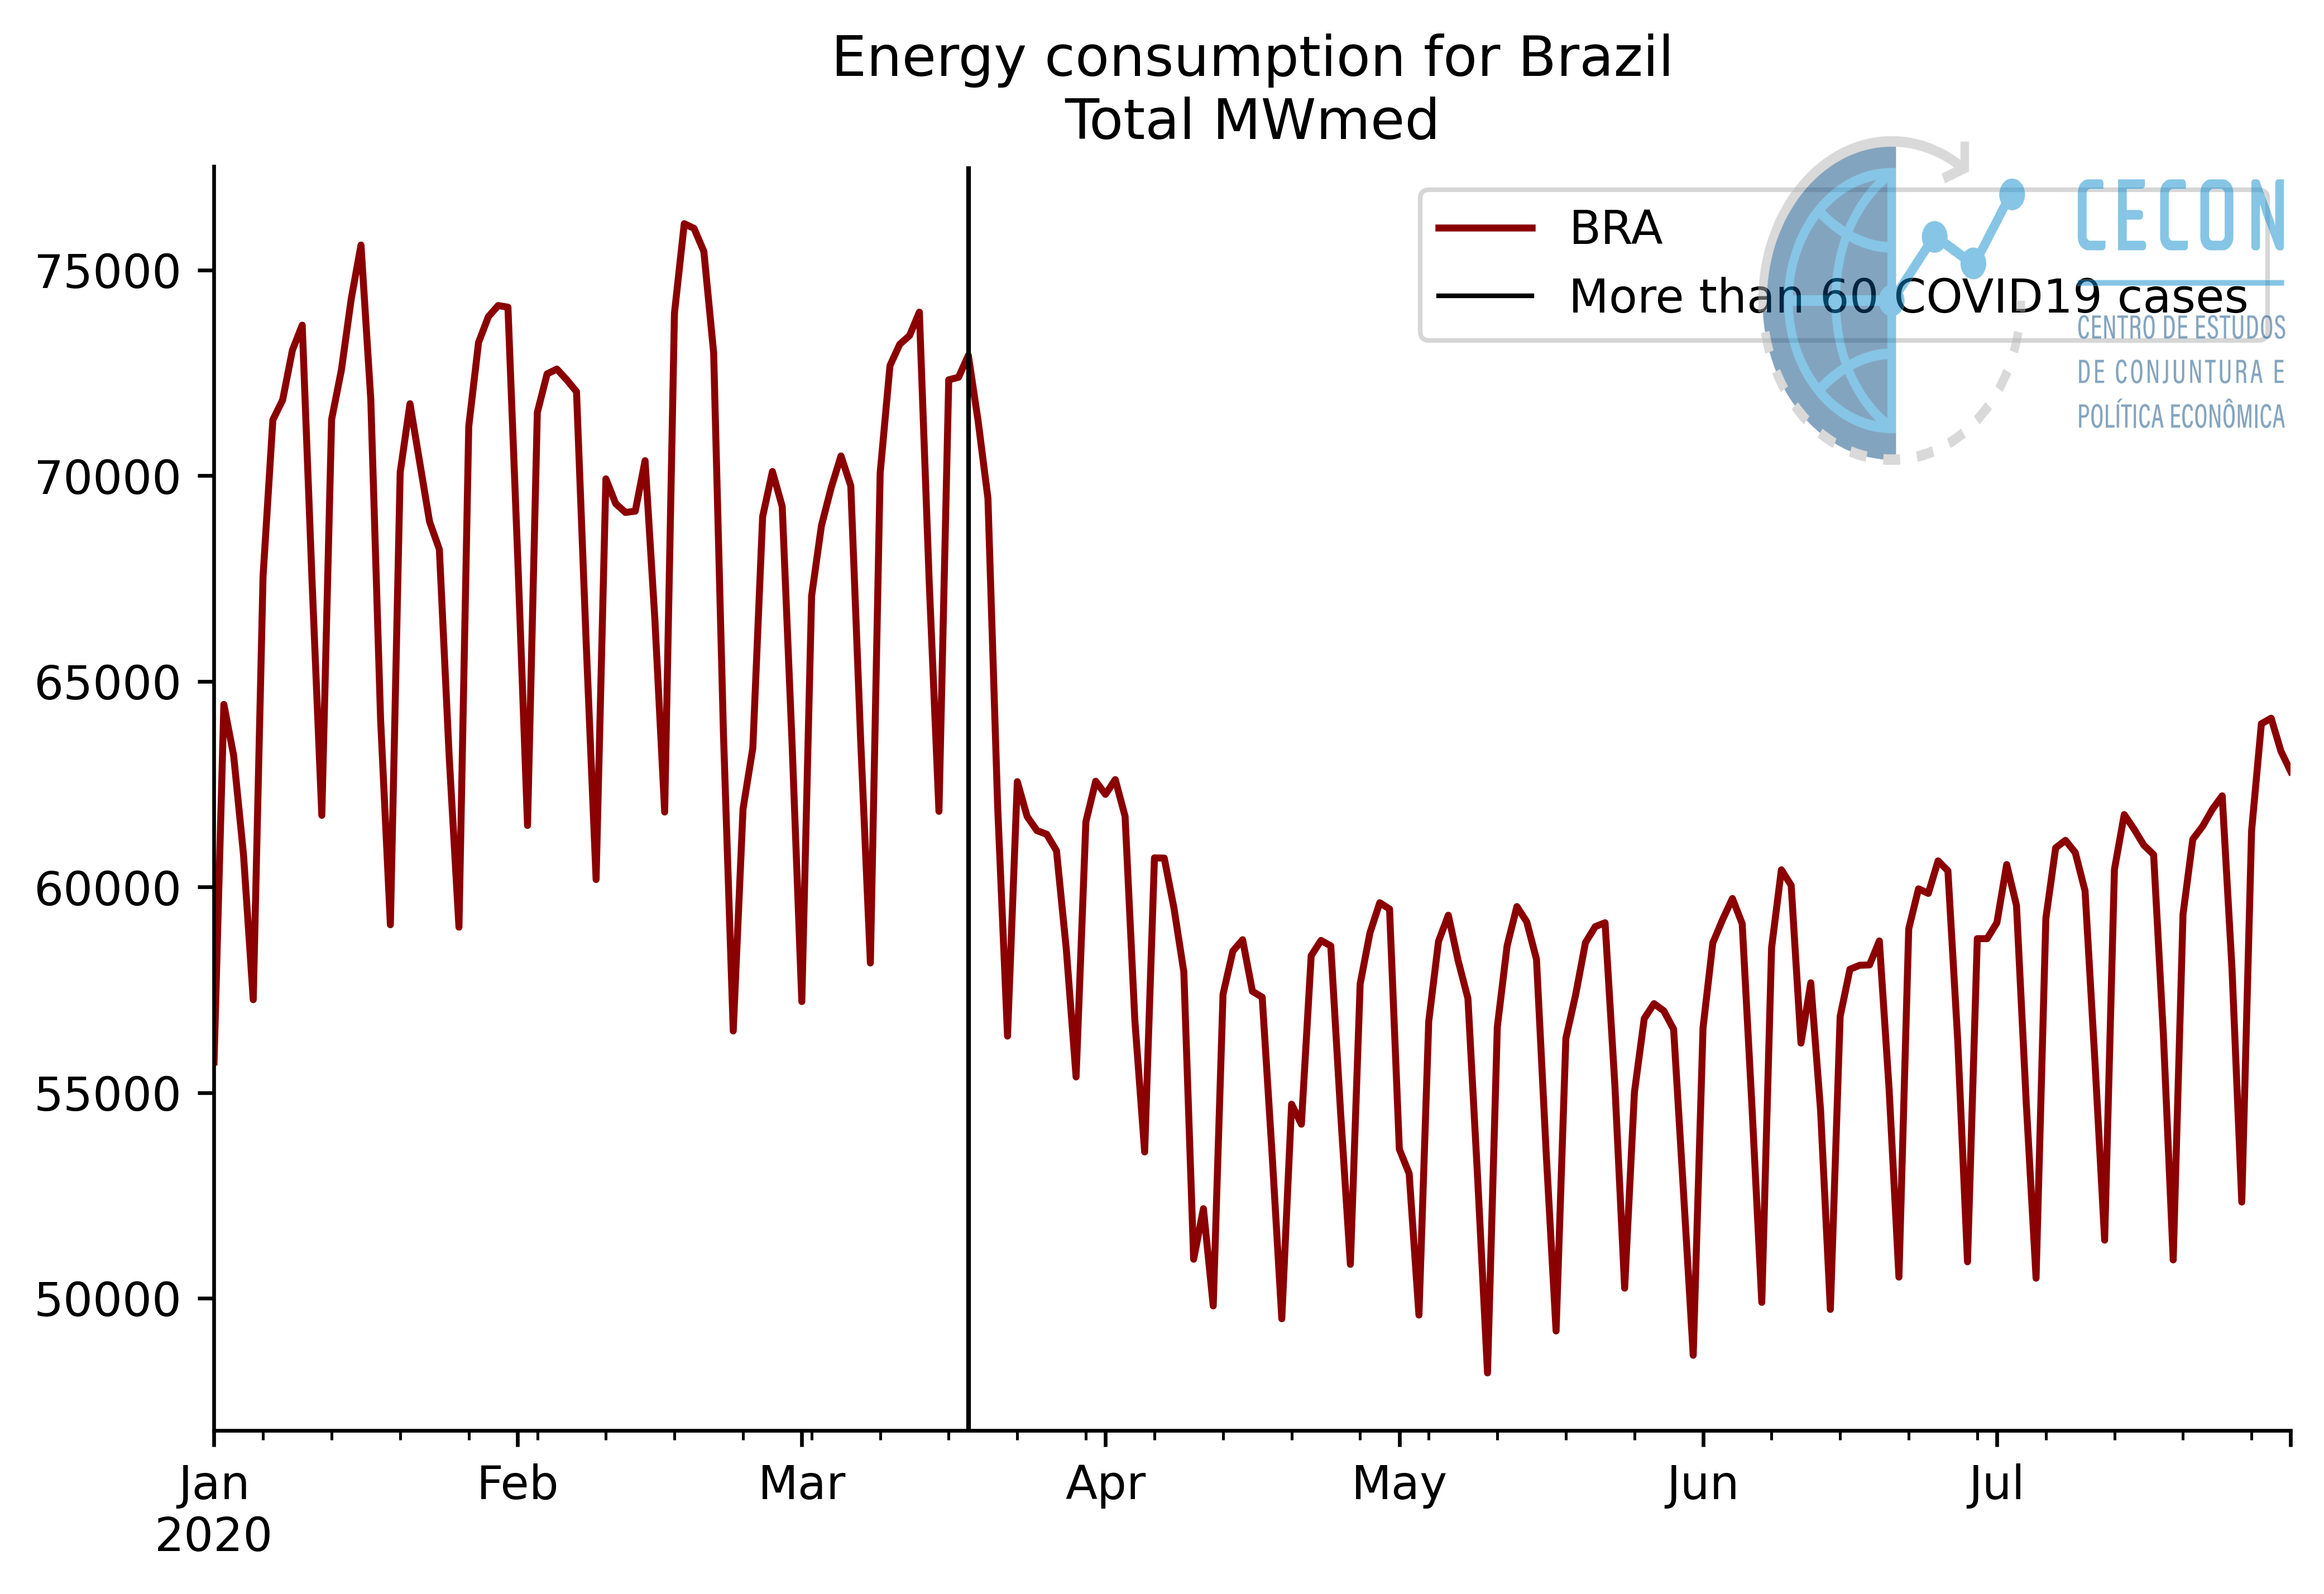
\includegraphics[width=.9\linewidth]{obipy-resources/62e383af79e91b63c7fc98dd7fb55b3c3ececcb9/77baa432ba2f44632060c841842355fcb8b83c23.png}
\end{center}

\begin{verbatim}
<Figure size 2400x1500 with 2 Axes>
\end{verbatim}


\begin{center}
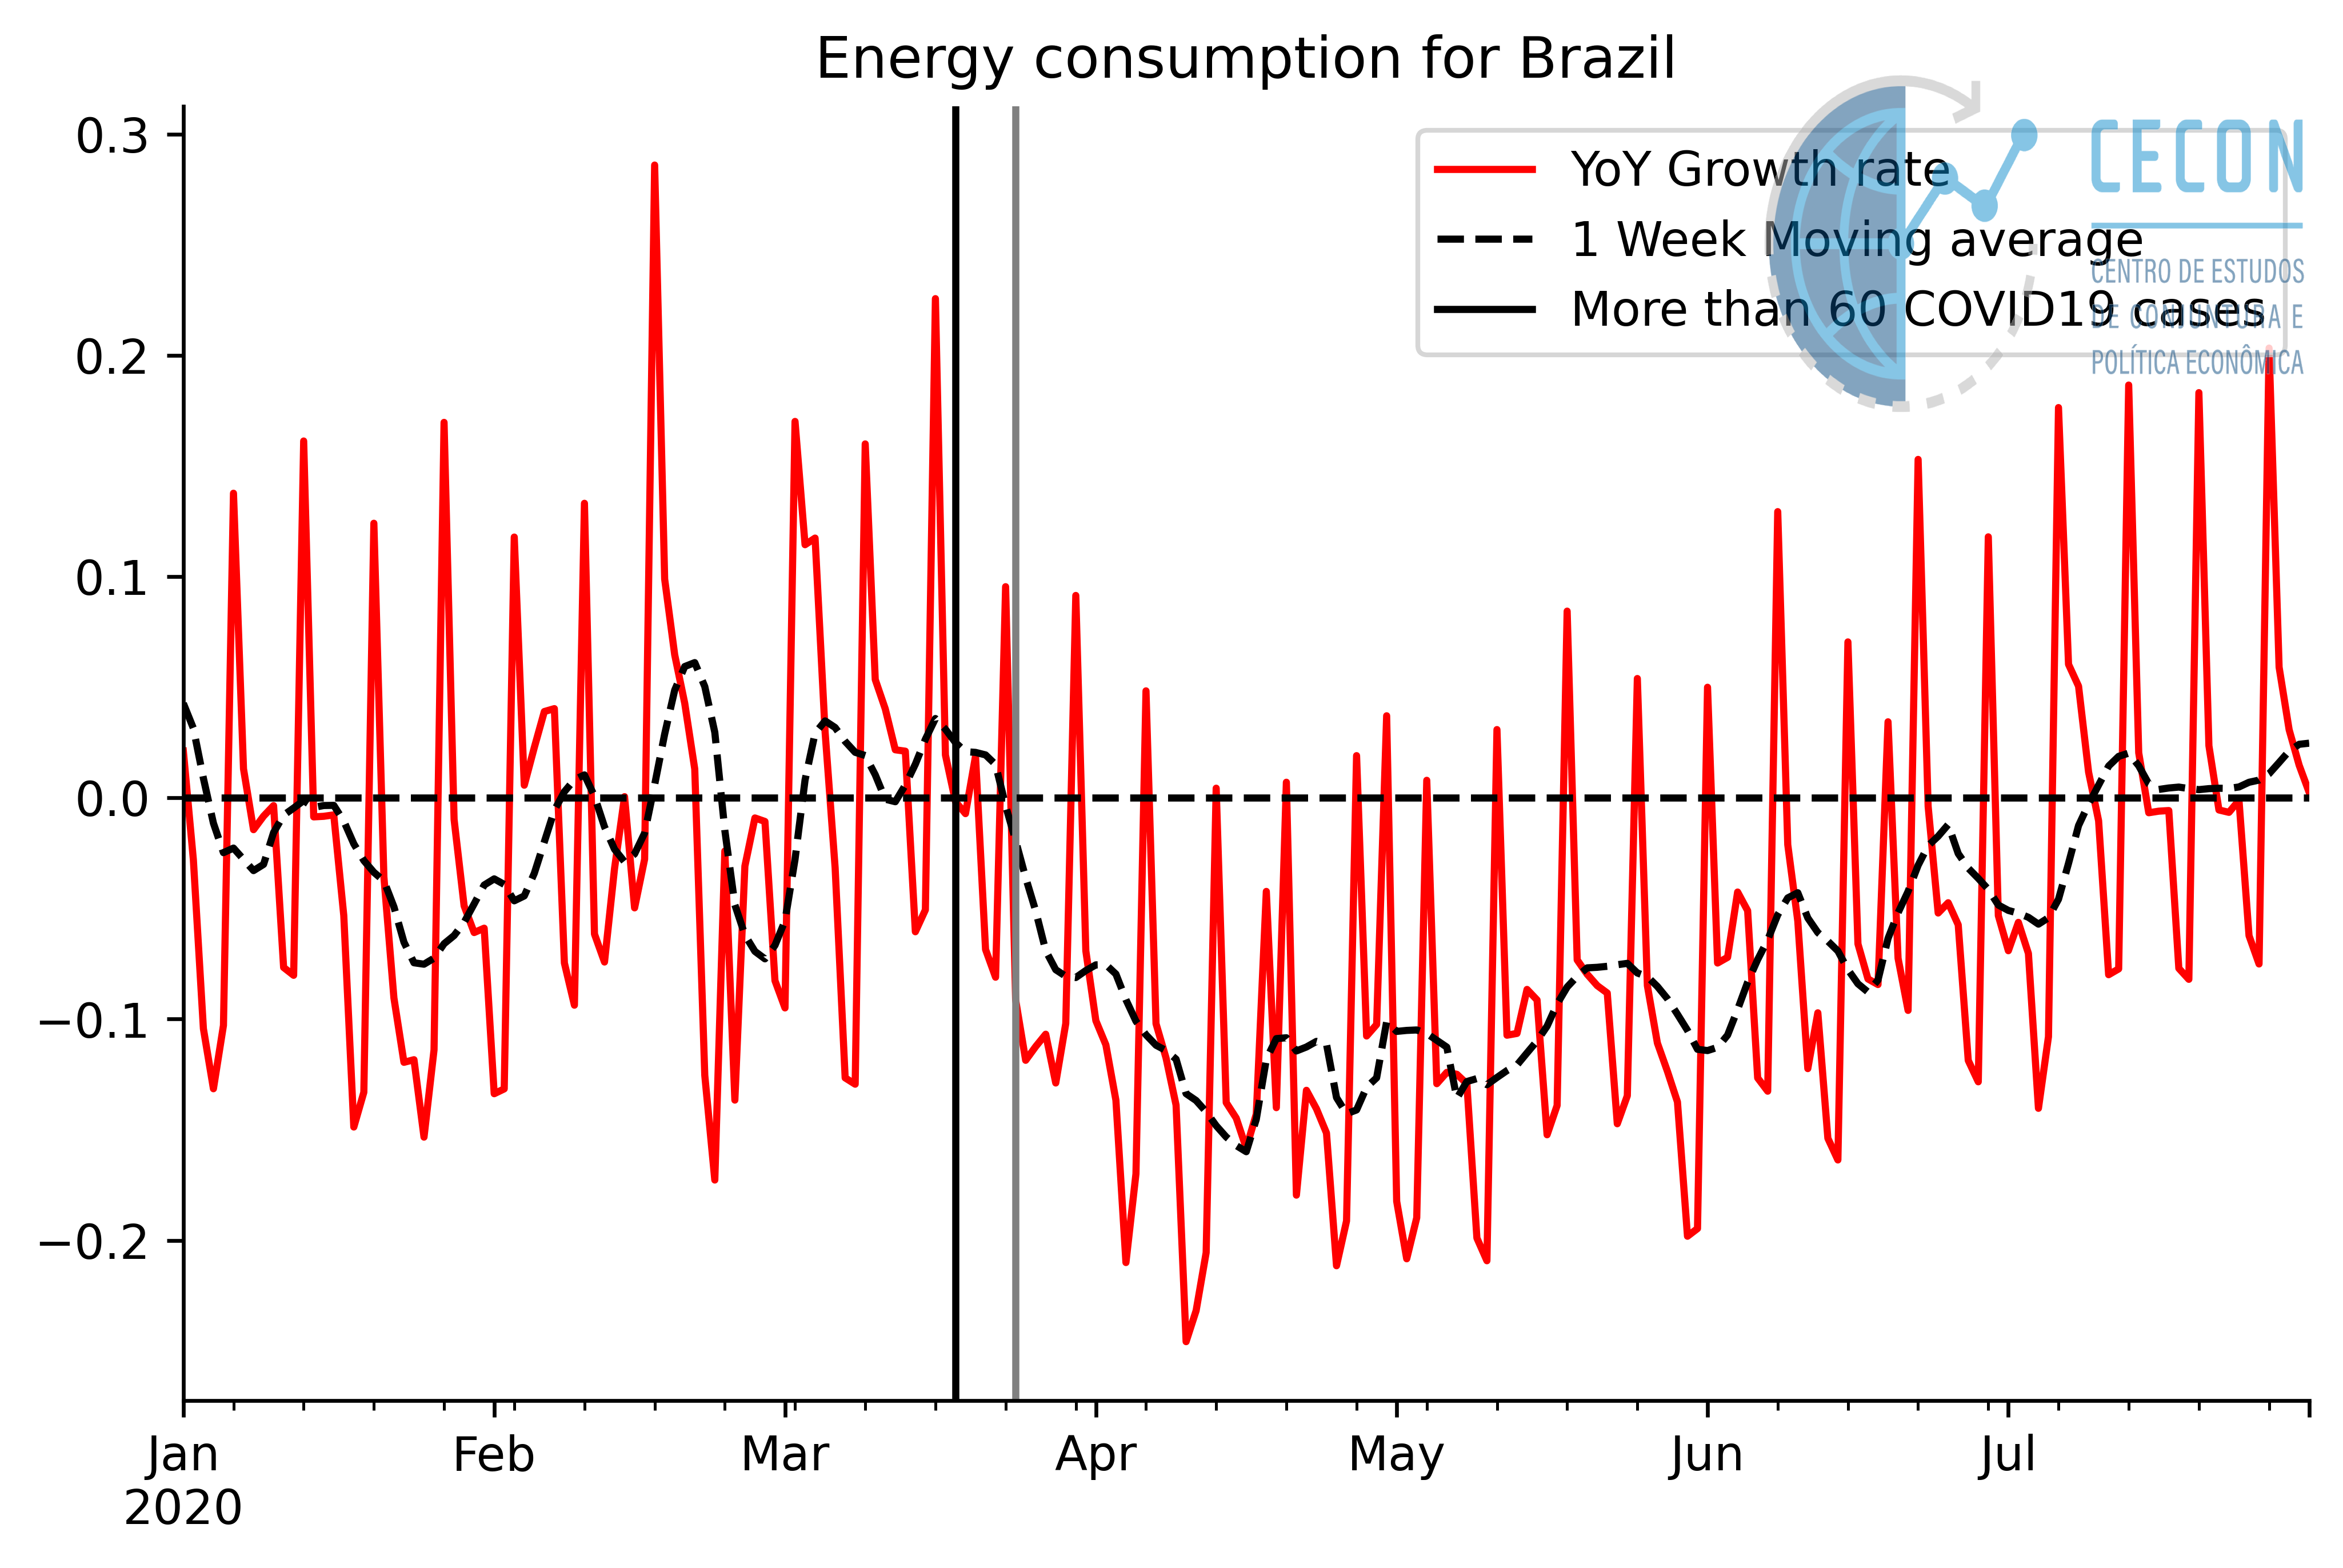
\includegraphics[width=.9\linewidth]{obipy-resources/62e383af79e91b63c7fc98dd7fb55b3c3ececcb9/d4289bac917b4c3c16dd2a44f65ca09392f8c087.png}
\end{center}

\begin{verbatim}
<Figure size 2400x1500 with 2 Axes>
\end{verbatim}


\begin{center}
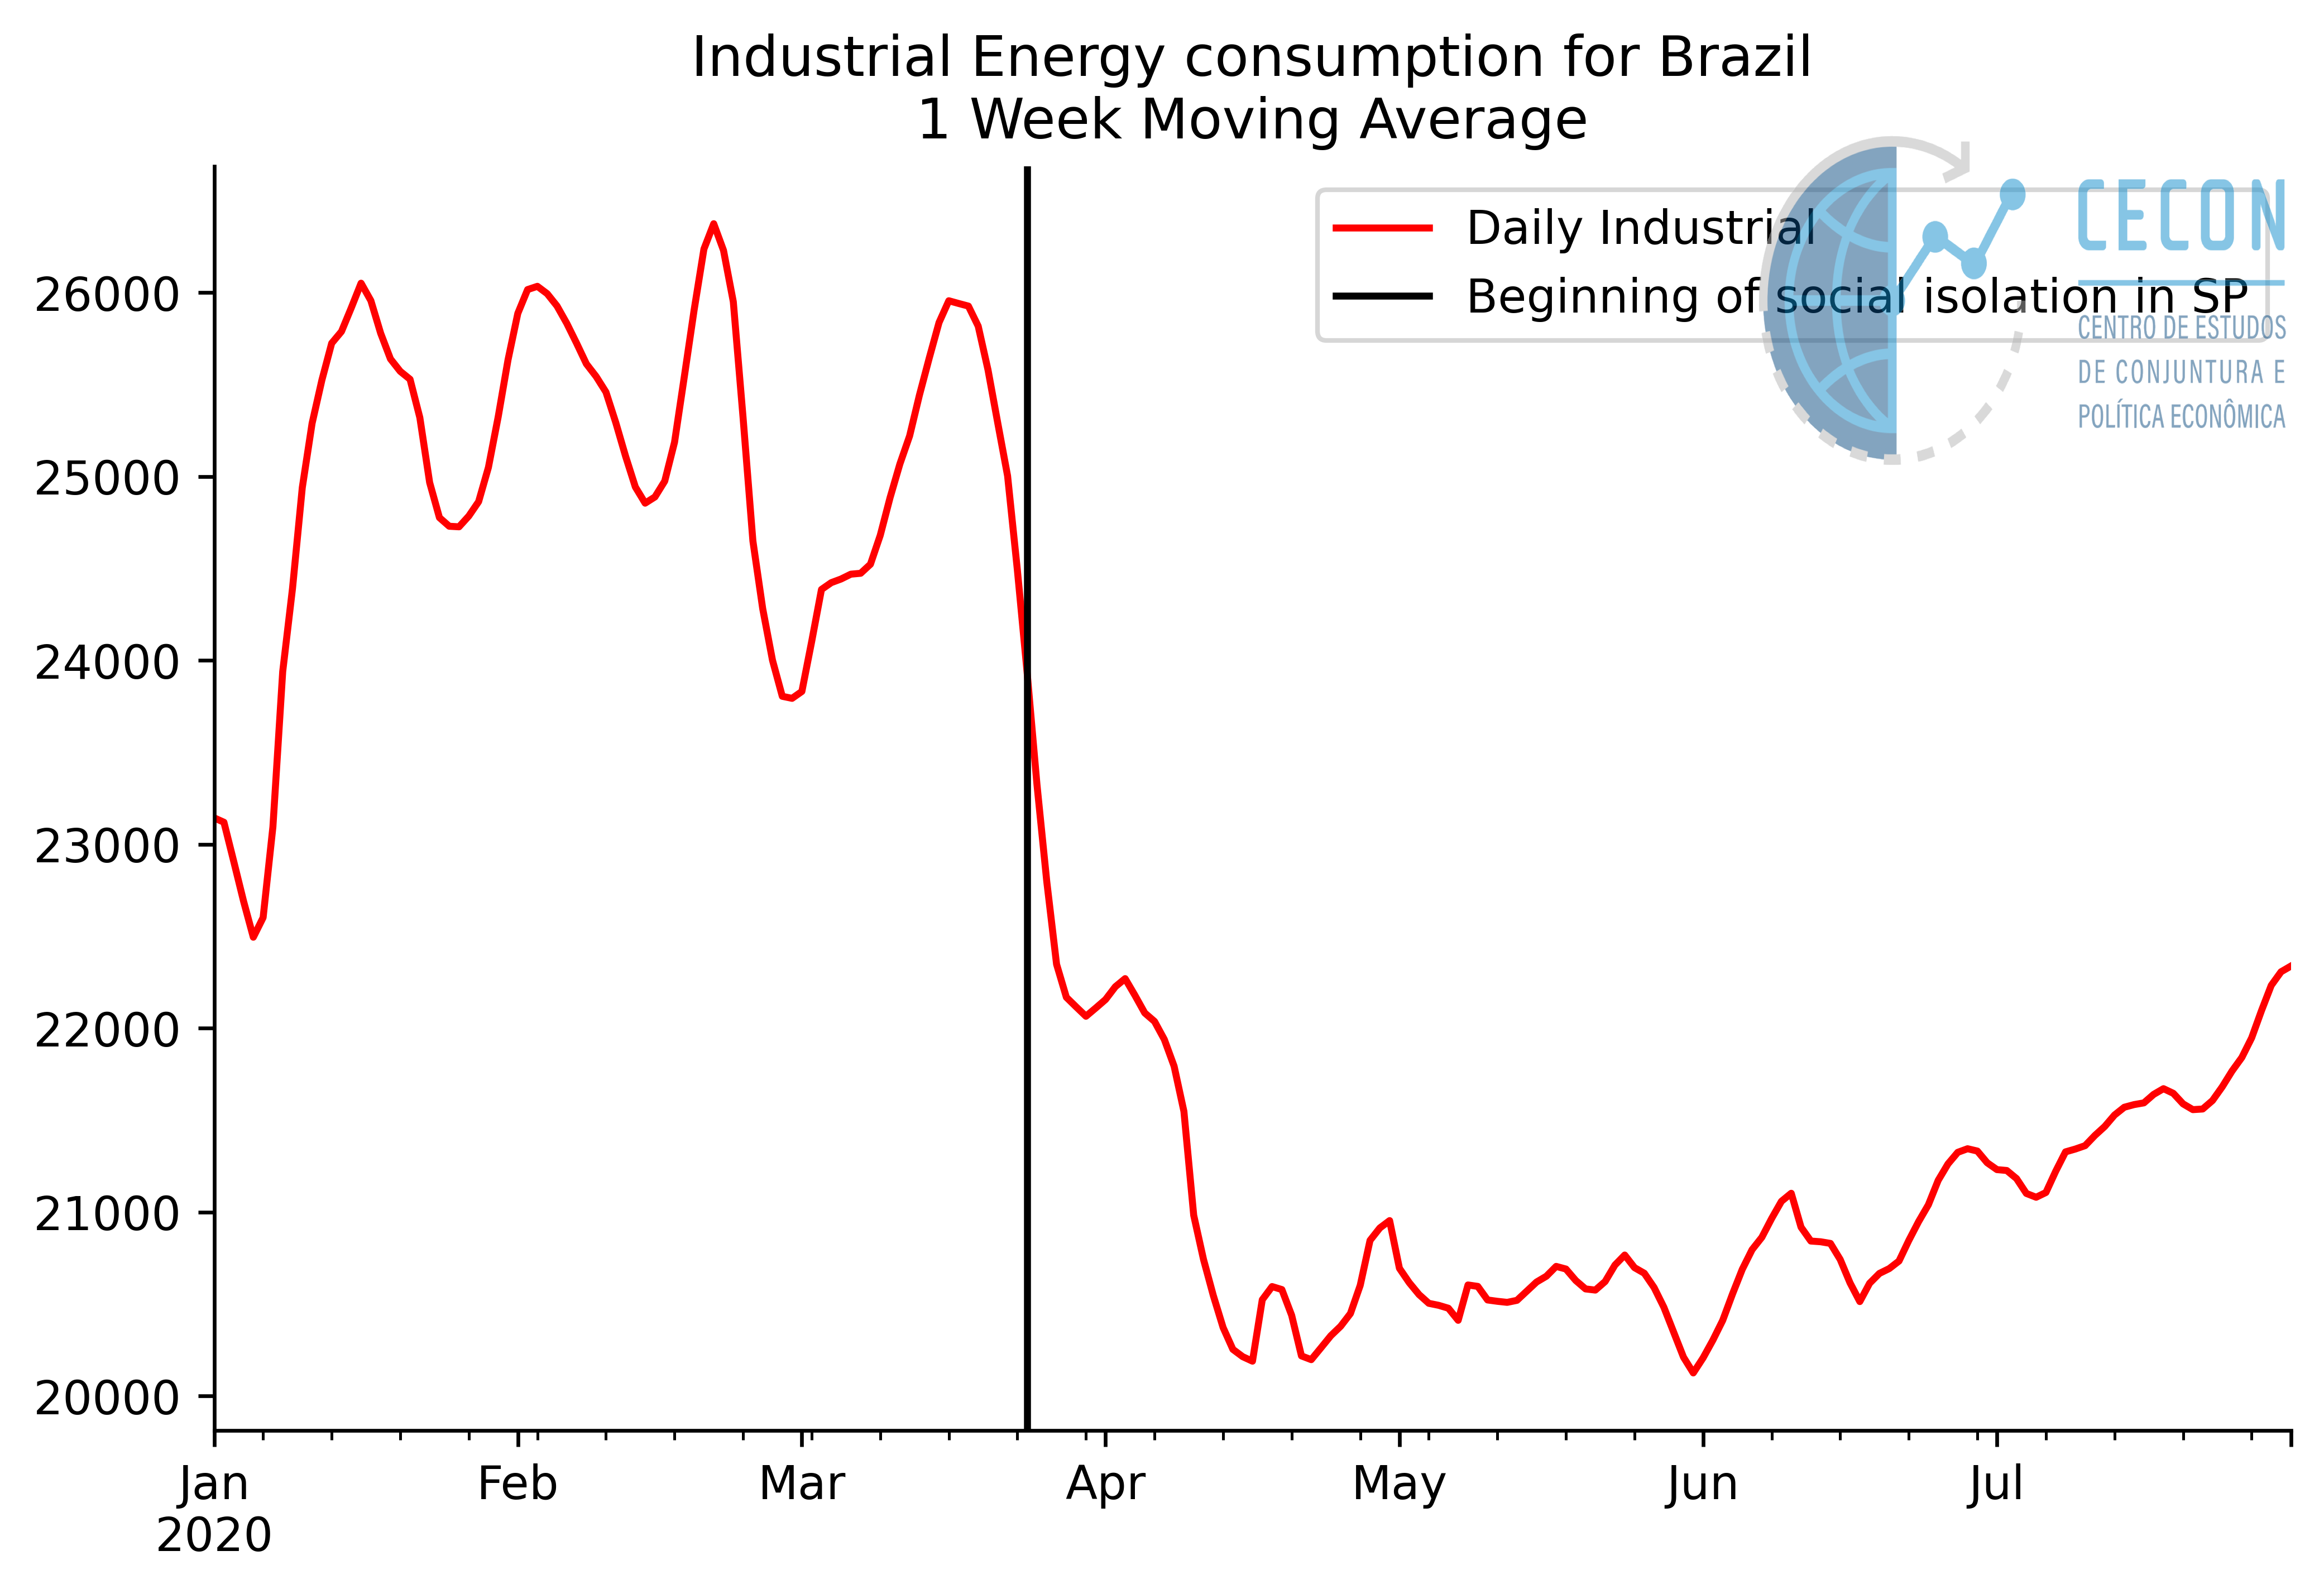
\includegraphics[width=.9\linewidth]{obipy-resources/62e383af79e91b63c7fc98dd7fb55b3c3ececcb9/bc952cb86ebe11930cccbfae0ee09821adb7b9c0.png}
\end{center}

\begin{verbatim}
<Figure size 2400x1500 with 2 Axes>
\end{verbatim}


\begin{center}
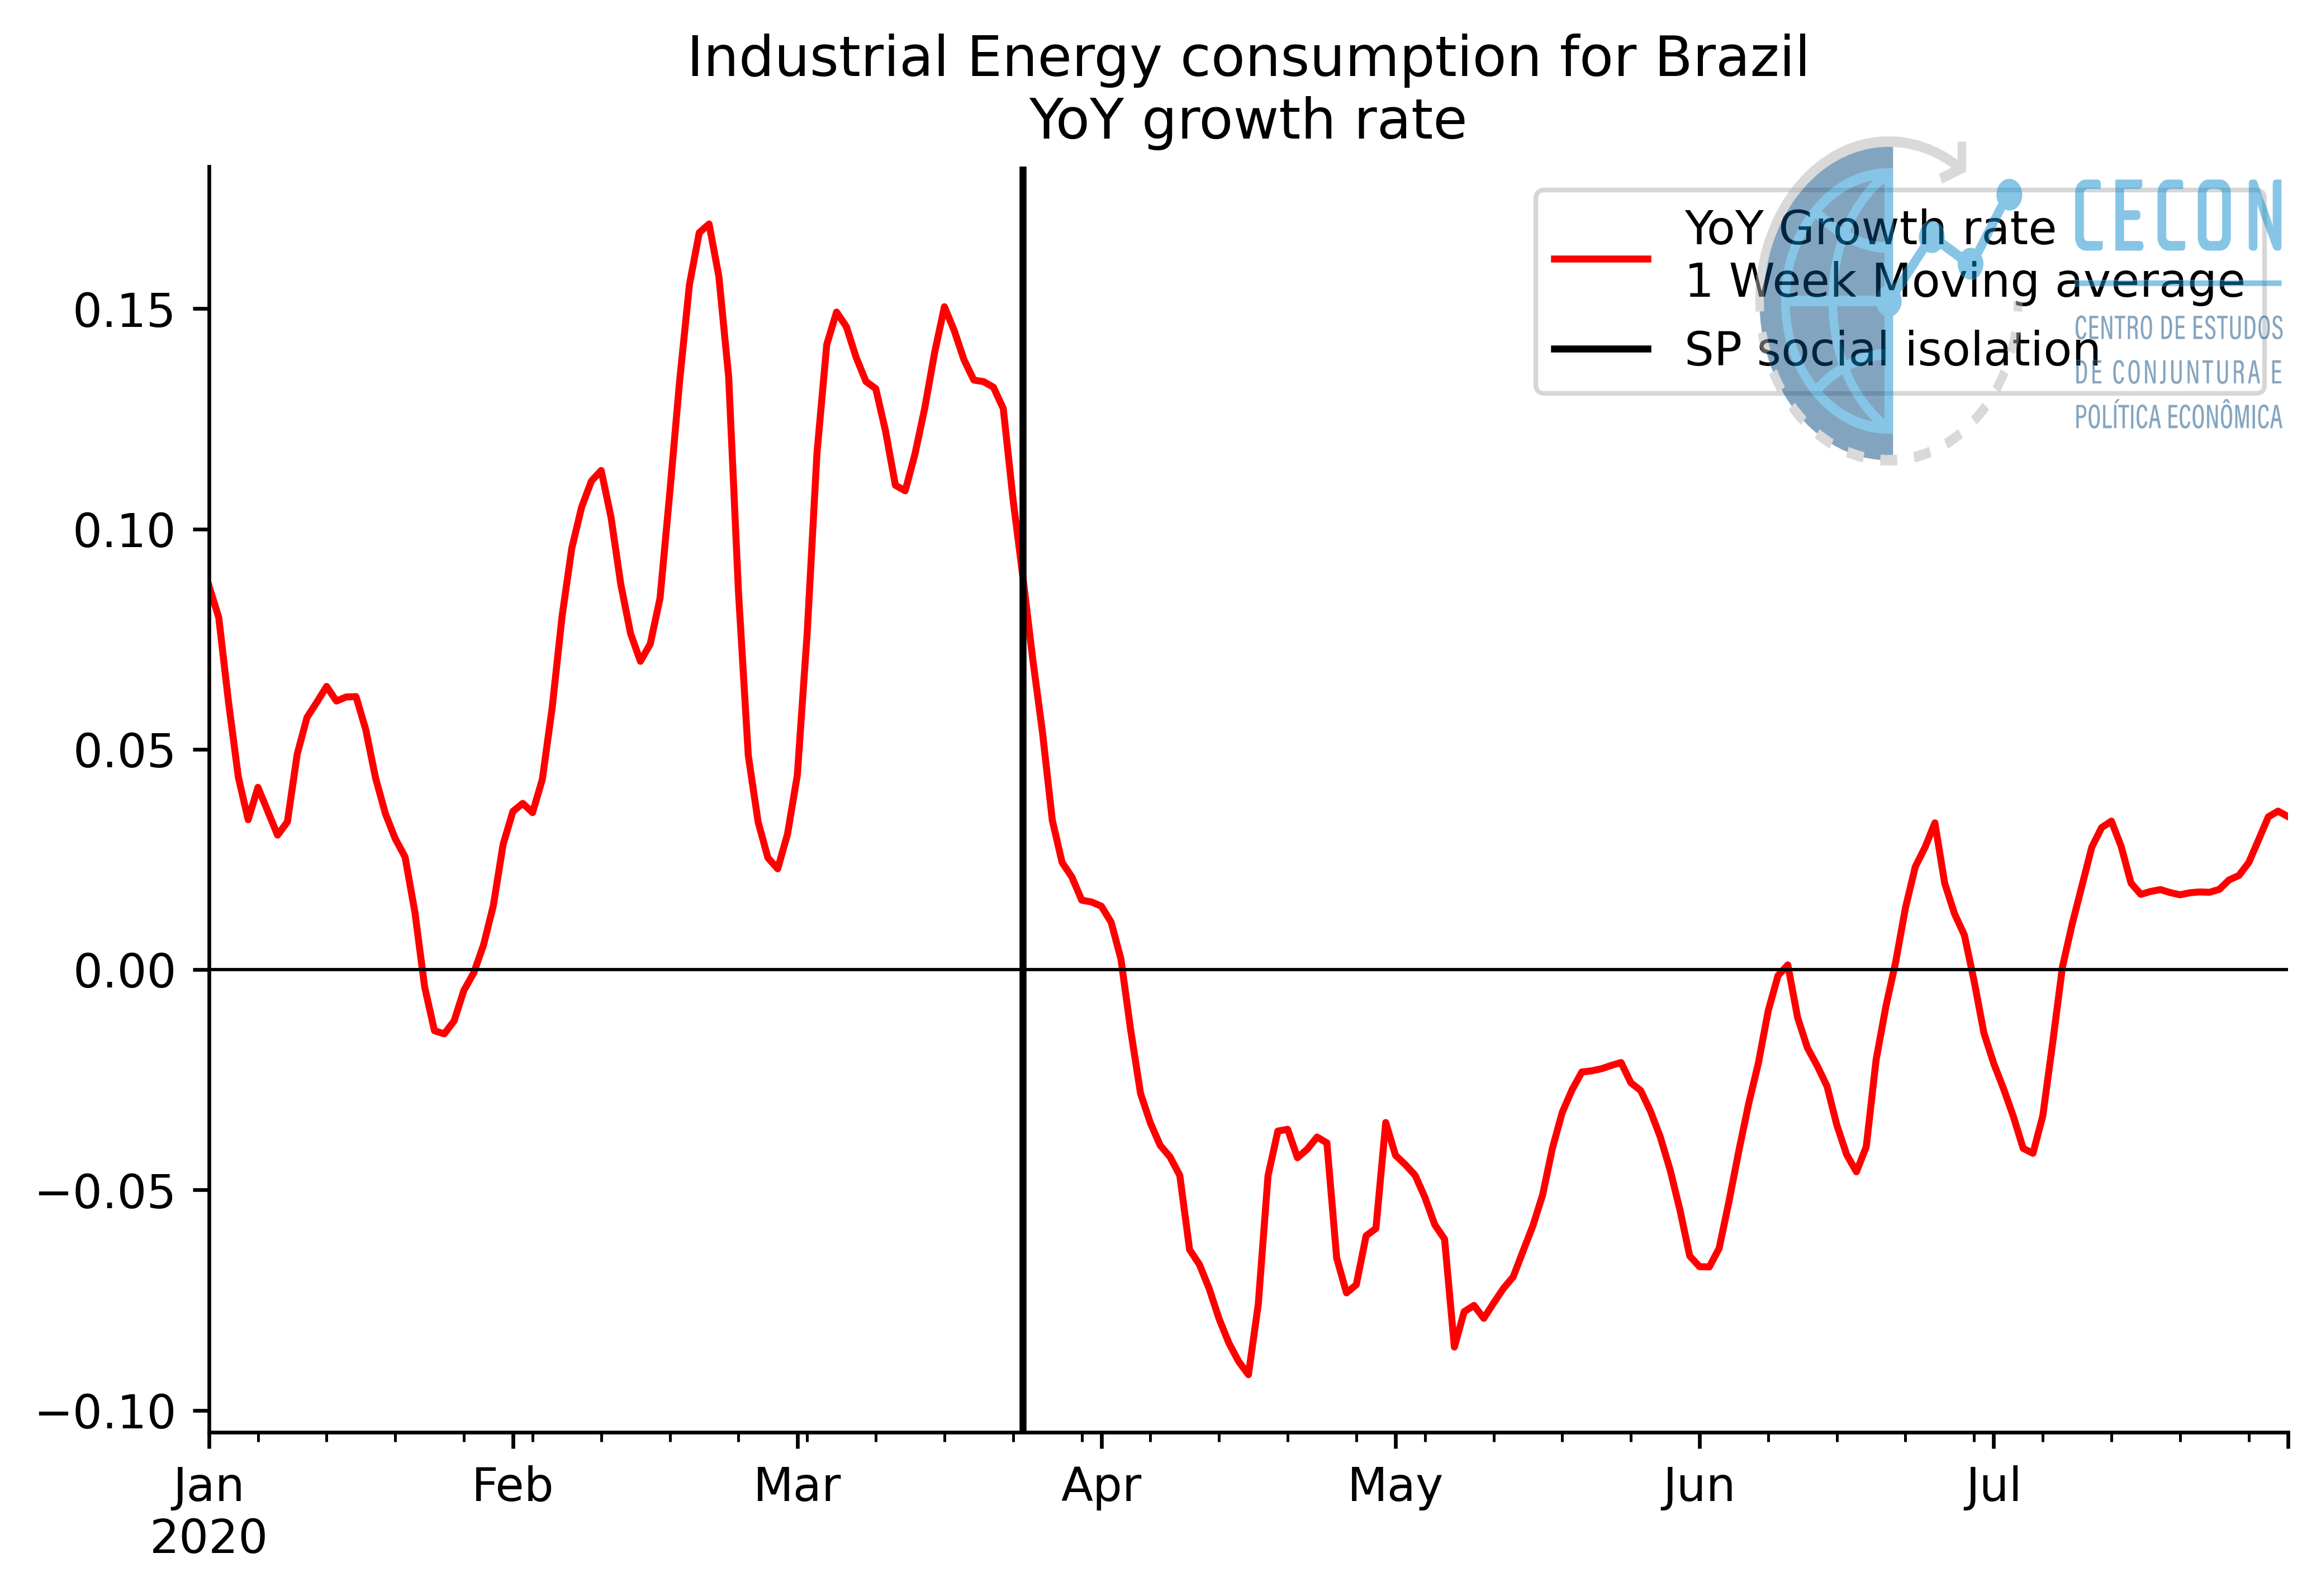
\includegraphics[width=.9\linewidth]{obipy-resources/62e383af79e91b63c7fc98dd7fb55b3c3ececcb9/f9ca7a33a86e705f7a59435db0037a8fc525f9eb.png}
\end{center}

\begin{verbatim}
<Figure size 2400x1500 with 2 Axes>
\end{verbatim}


\begin{center}
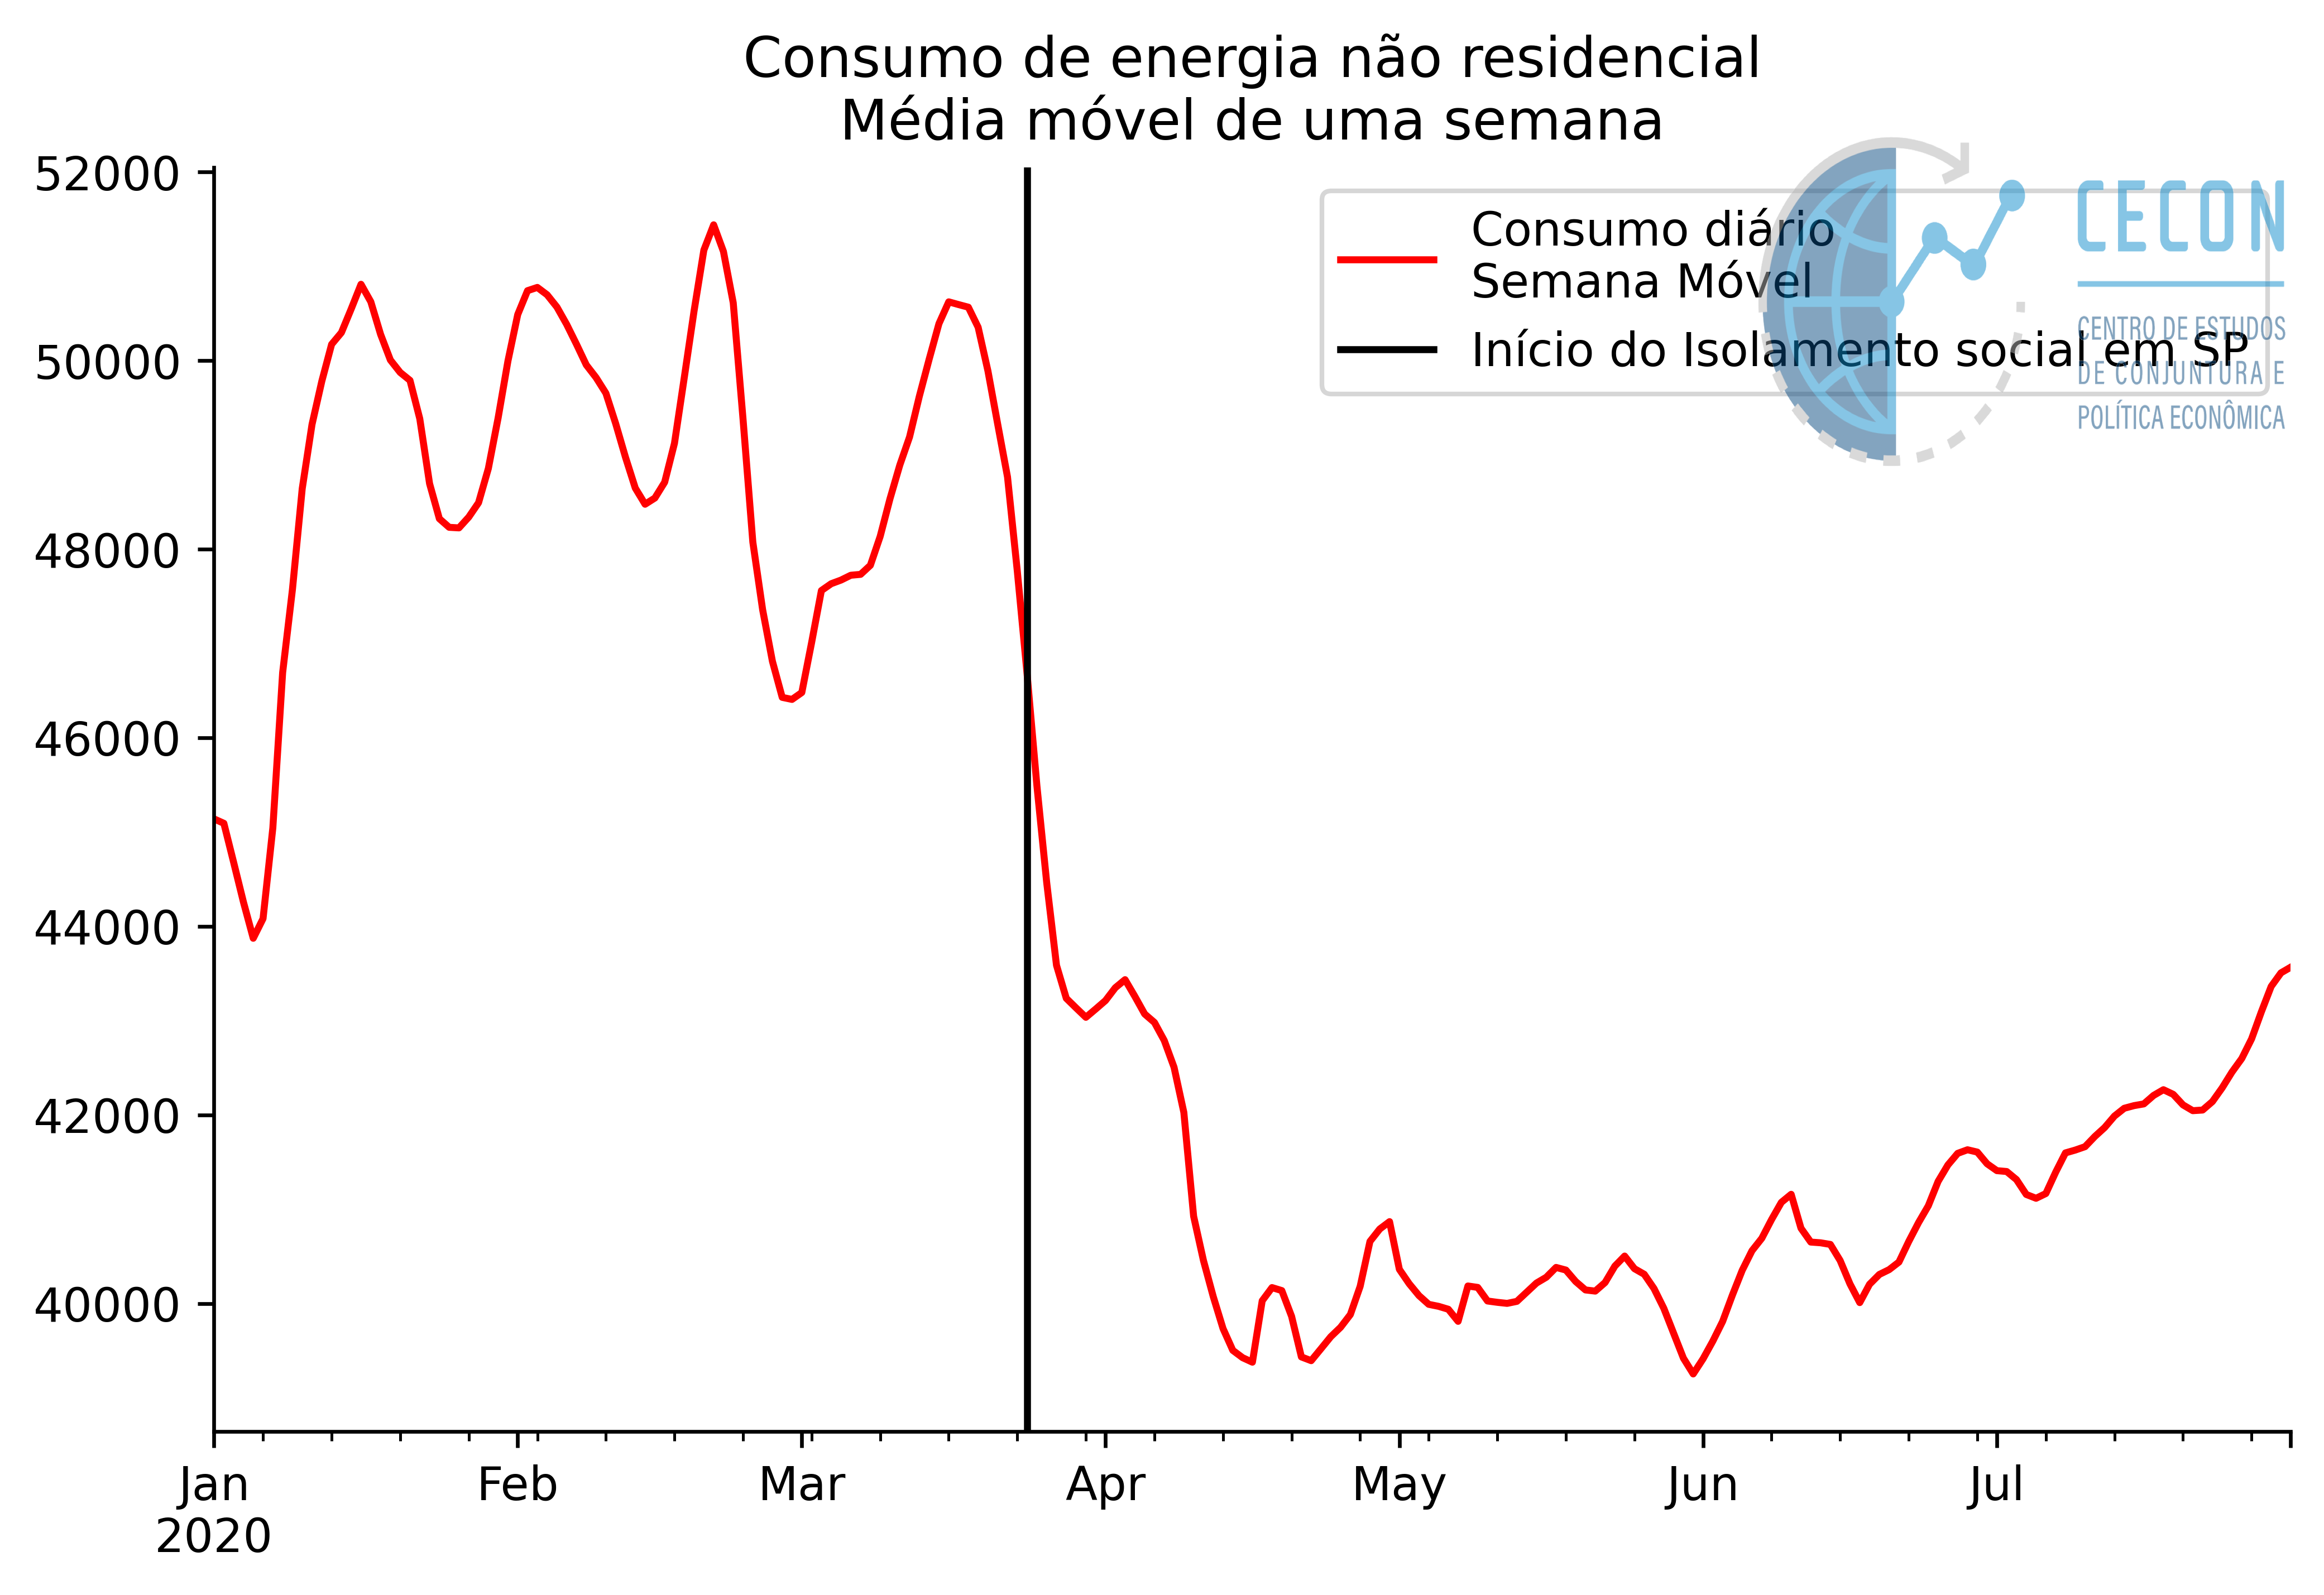
\includegraphics[width=.9\linewidth]{obipy-resources/62e383af79e91b63c7fc98dd7fb55b3c3ececcb9/3f4b22b7fe301e9d040661b4ccbfccd82d0f77ff.png}
\end{center}

\begin{verbatim}
<Figure size 2400x1500 with 2 Axes>
\end{verbatim}


\begin{center}
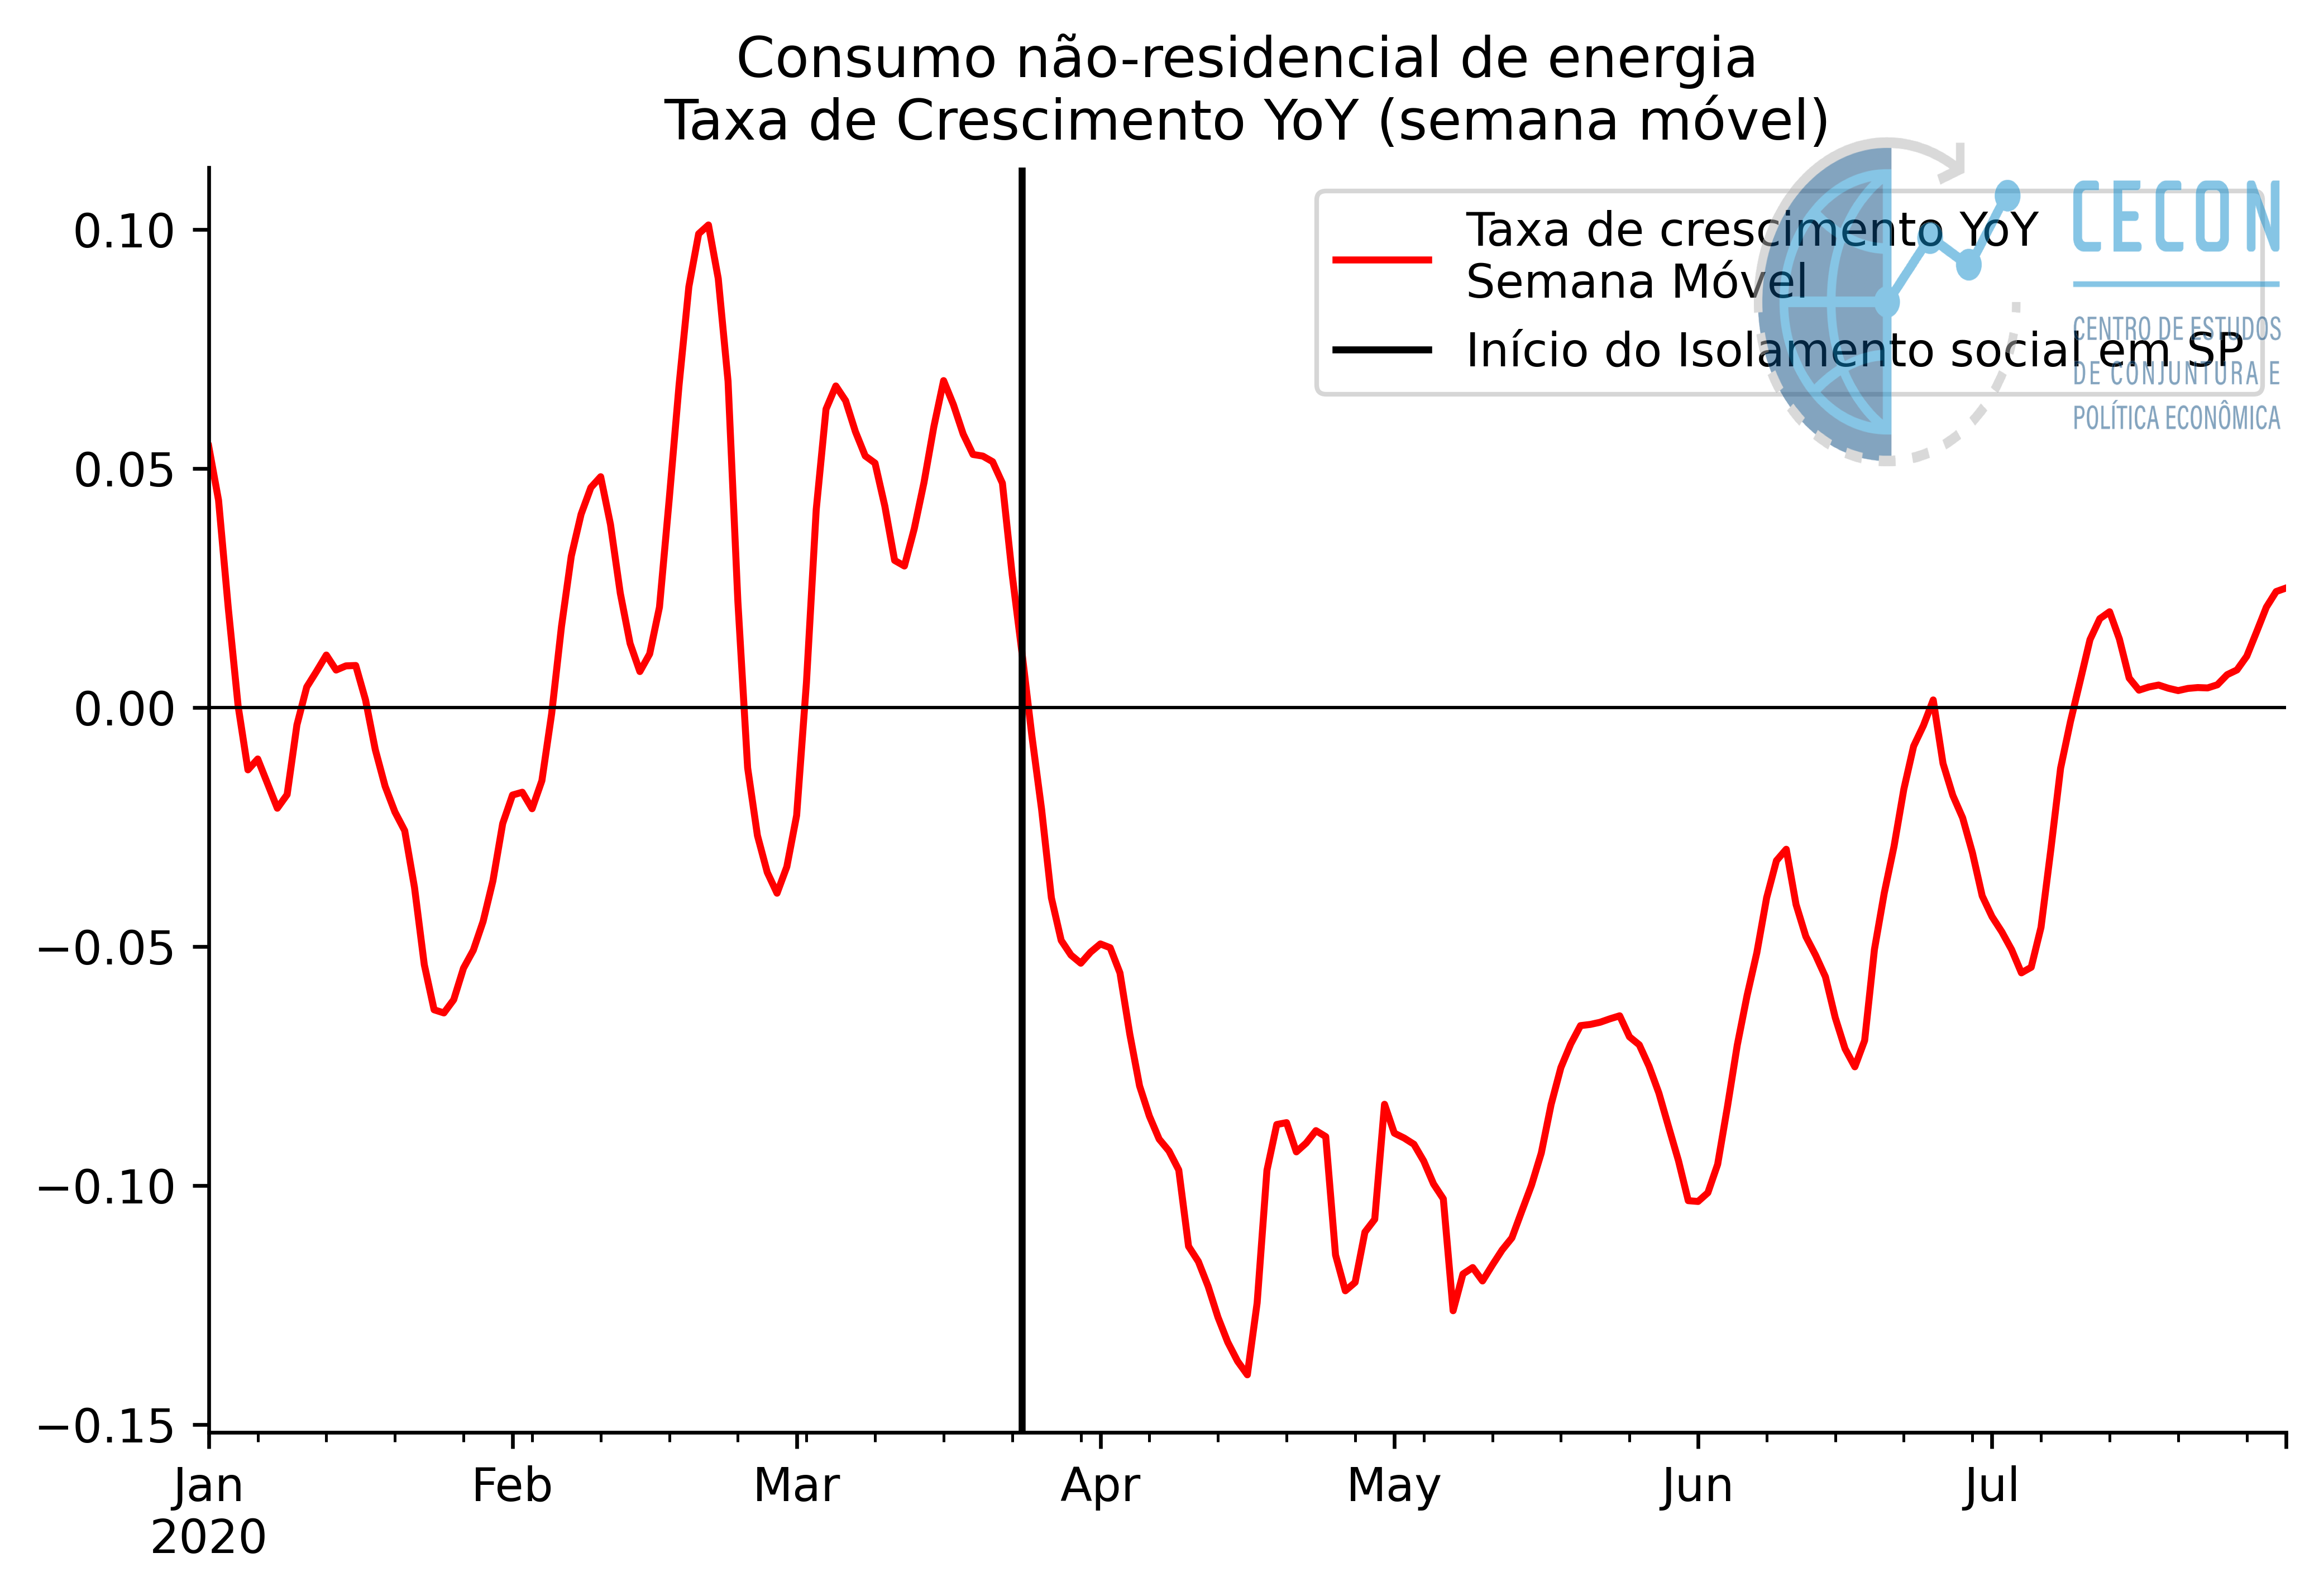
\includegraphics[width=.9\linewidth]{obipy-resources/62e383af79e91b63c7fc98dd7fb55b3c3ececcb9/862628f923a3fda24d4e664ce8bc872a805019fe.png}
\end{center}
\end{enumerate}




\subsubsection{France: FRA}
\label{sec:orge88c274}

<ipython-input-21-06392b792fc4>:74: UserWarning: This figure includes Axes that are not compatible with tight\_layout, so results might be incorrect.
  plt.tight\_layout()

\begin{verbatim}
<Figure size 2400x1500 with 4 Axes>
\end{verbatim}


\begin{center}
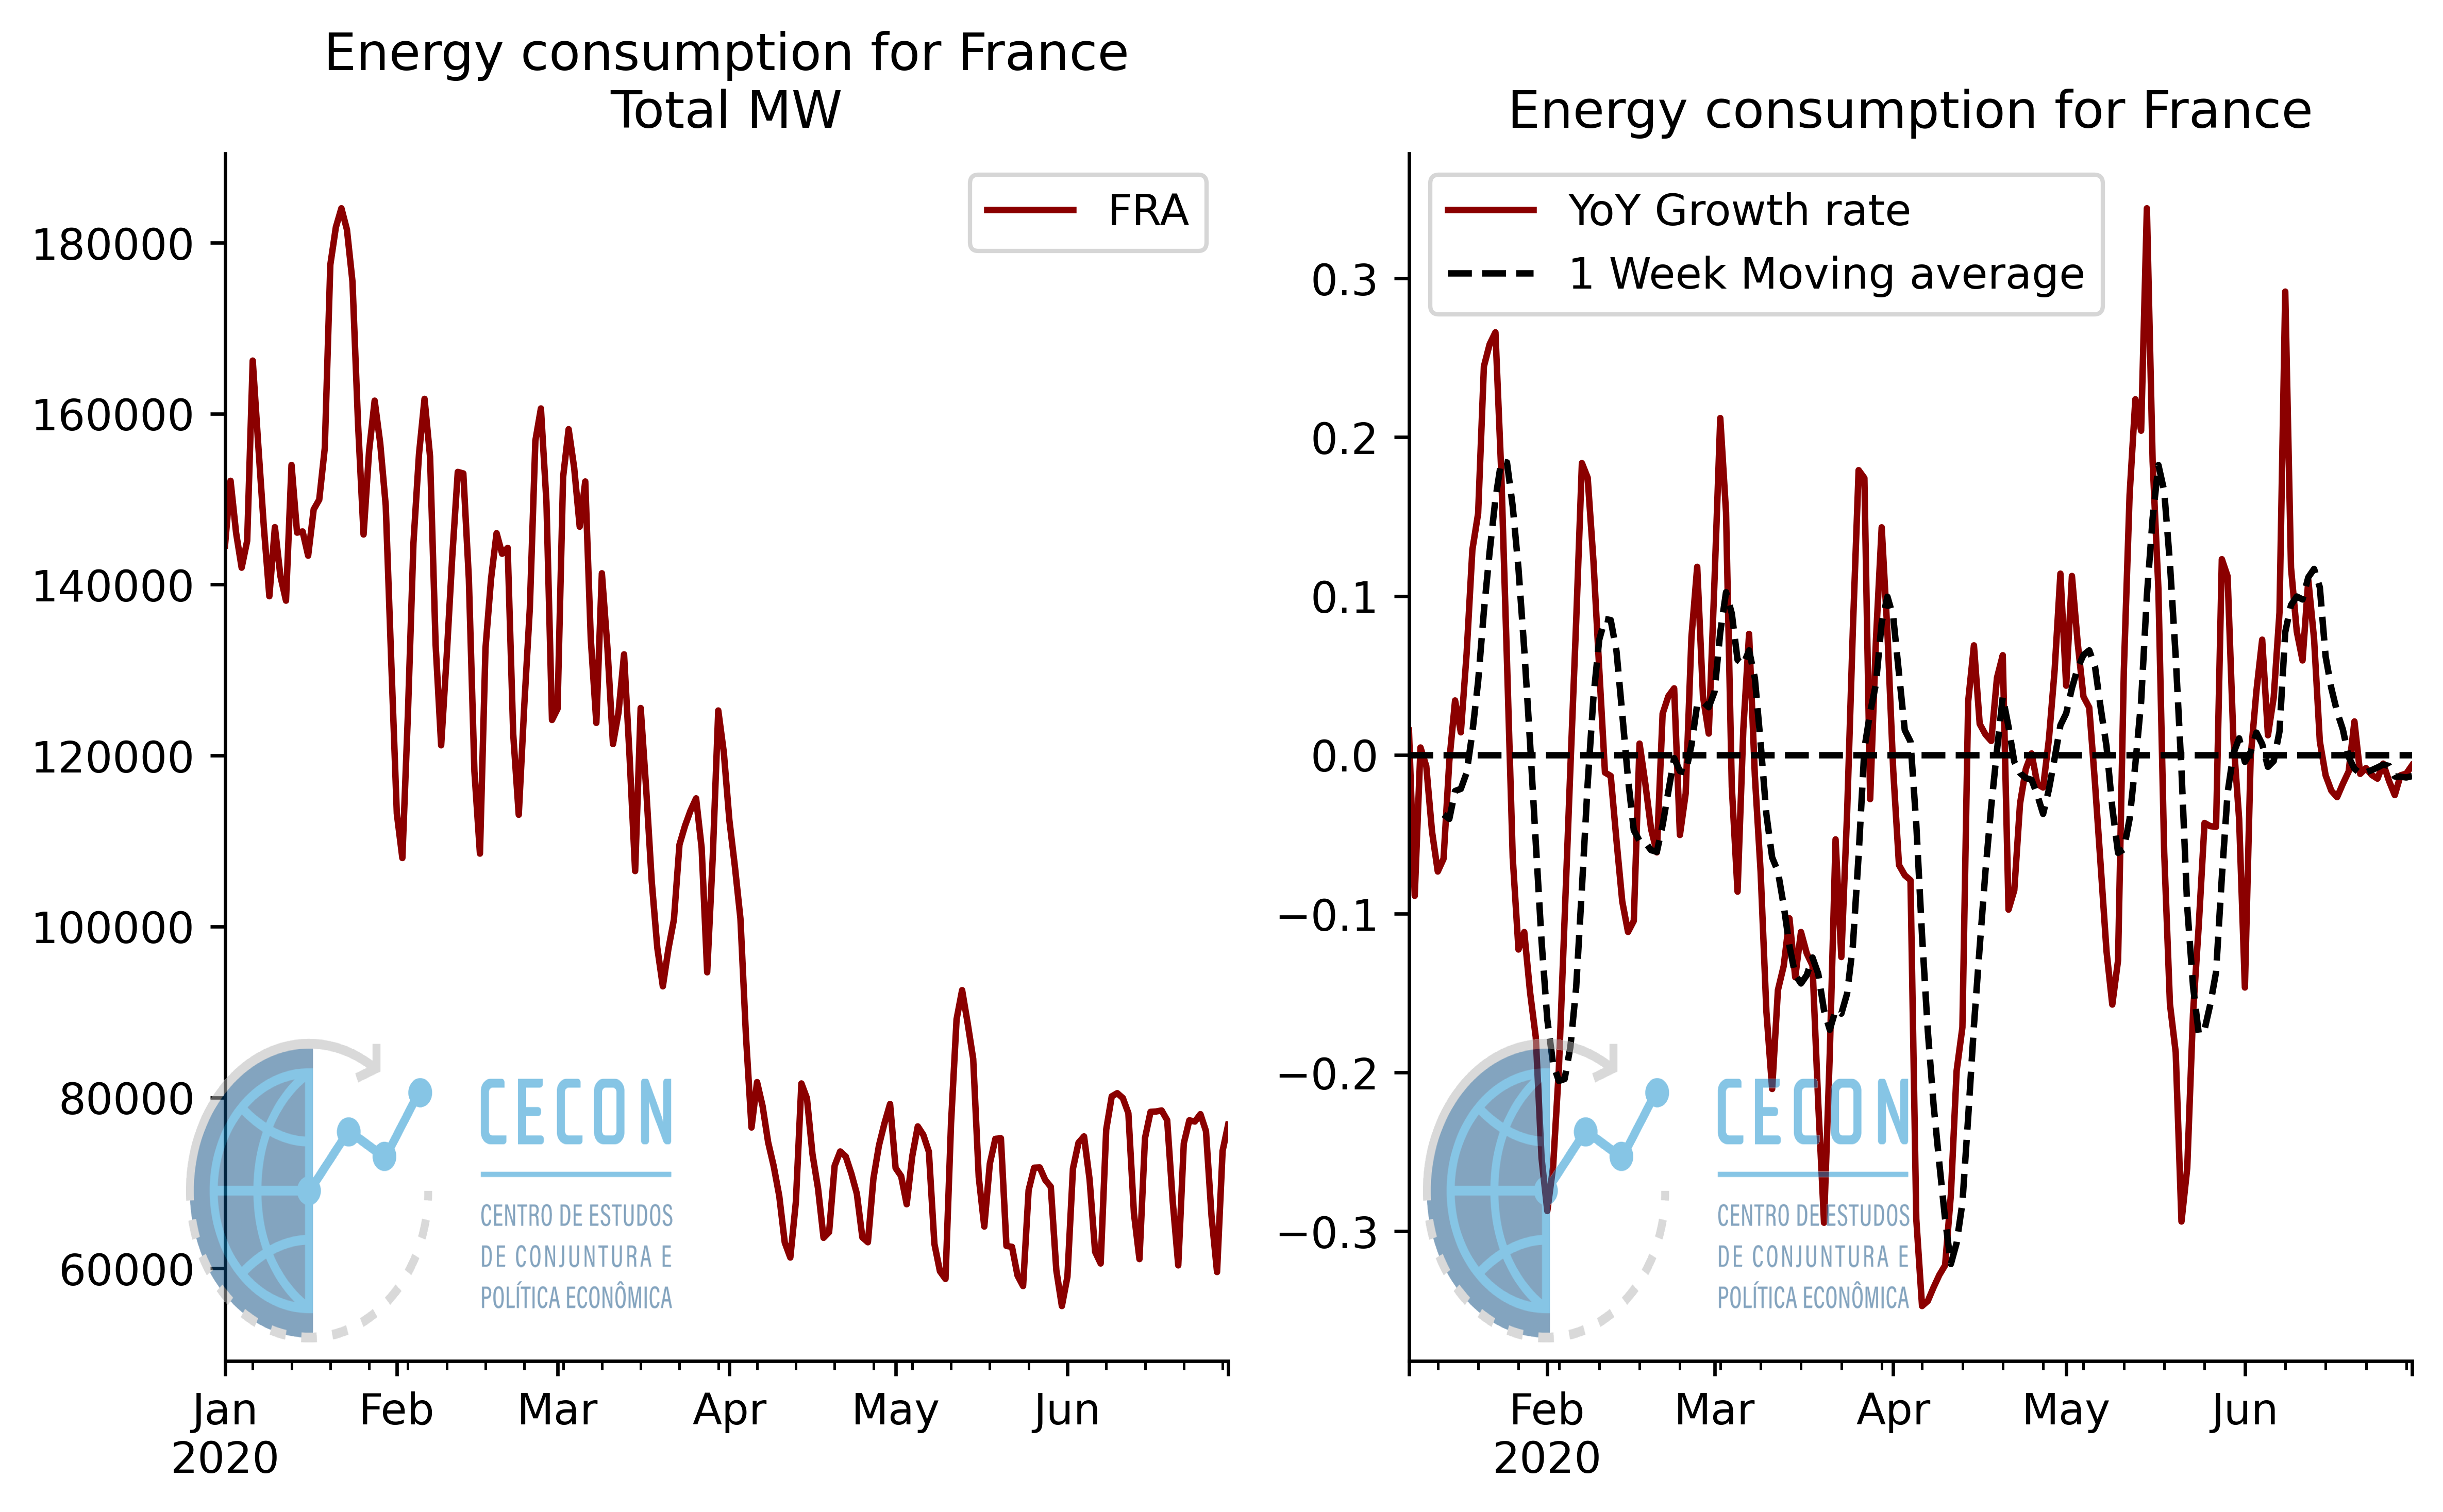
\includegraphics[width=.9\linewidth]{obipy-resources/62e383af79e91b63c7fc98dd7fb55b3c3ececcb9/325746abff053090d5f6fe9490ccdb4ba397472d.png}
\end{center}

\subsubsection{Spain: Spain}
\label{sec:orgd1ad82d}

\textbf{Corrigir}

<ipython-input-21-06392b792fc4>:74: UserWarning: This figure includes Axes that are not compatible with tight\_layout, so results might be incorrect.
  plt.tight\_layout()

\begin{verbatim}
<Figure size 2400x1500 with 4 Axes>
\end{verbatim}


\begin{center}
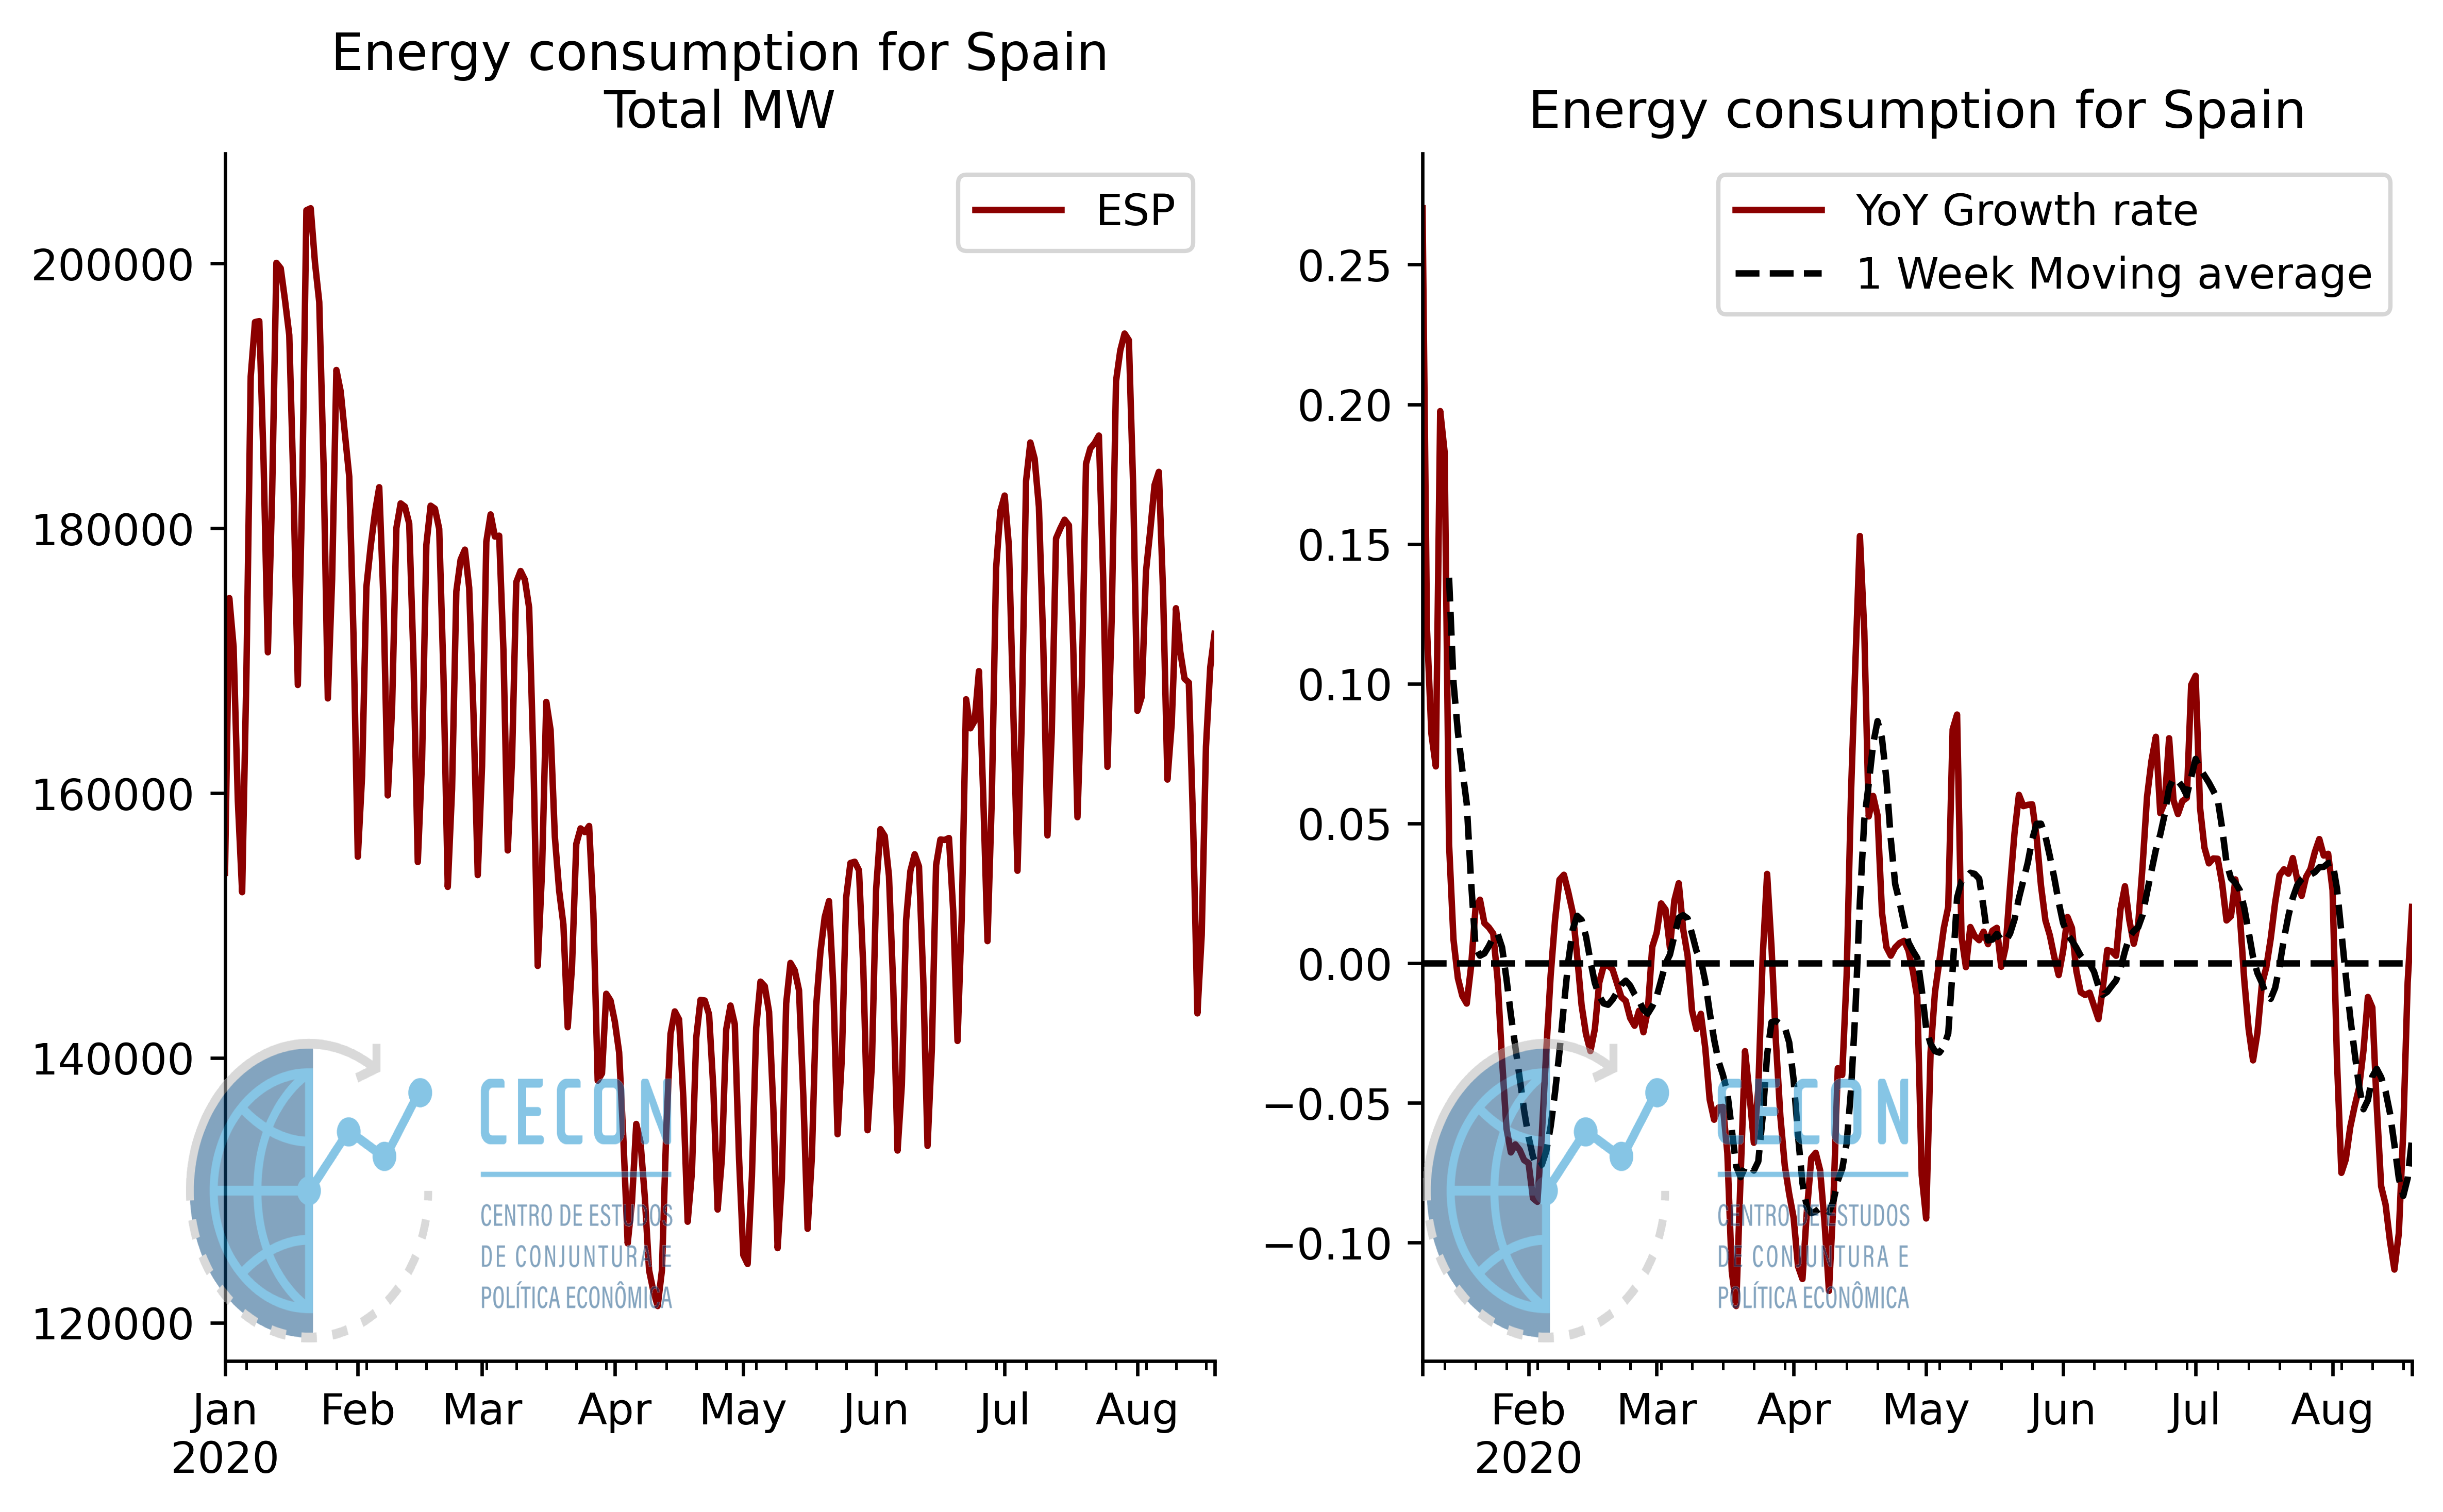
\includegraphics[width=.9\linewidth]{obipy-resources/62e383af79e91b63c7fc98dd7fb55b3c3ececcb9/aa615addfd95d863842bc30c5c6c024b67813166.png}
\end{center}

\subsubsection{Austria: AUS}
\label{sec:org6b94274}

<ipython-input-21-06392b792fc4>:74: UserWarning: This figure includes Axes that are not compatible with tight\_layout, so results might be incorrect.
  plt.tight\_layout()

\begin{verbatim}
(<Figure size 2400x1500 with 4 Axes>,
 array([<matplotlib.axes._subplots.AxesSubplot object at 0x7f69c9727190>,
        <matplotlib.axes._subplots.AxesSubplot object at 0x7f69cbec3400>],
       dtype=object))
\end{verbatim}


\begin{verbatim}
<Figure size 2400x1500 with 4 Axes>
\end{verbatim}


\begin{center}
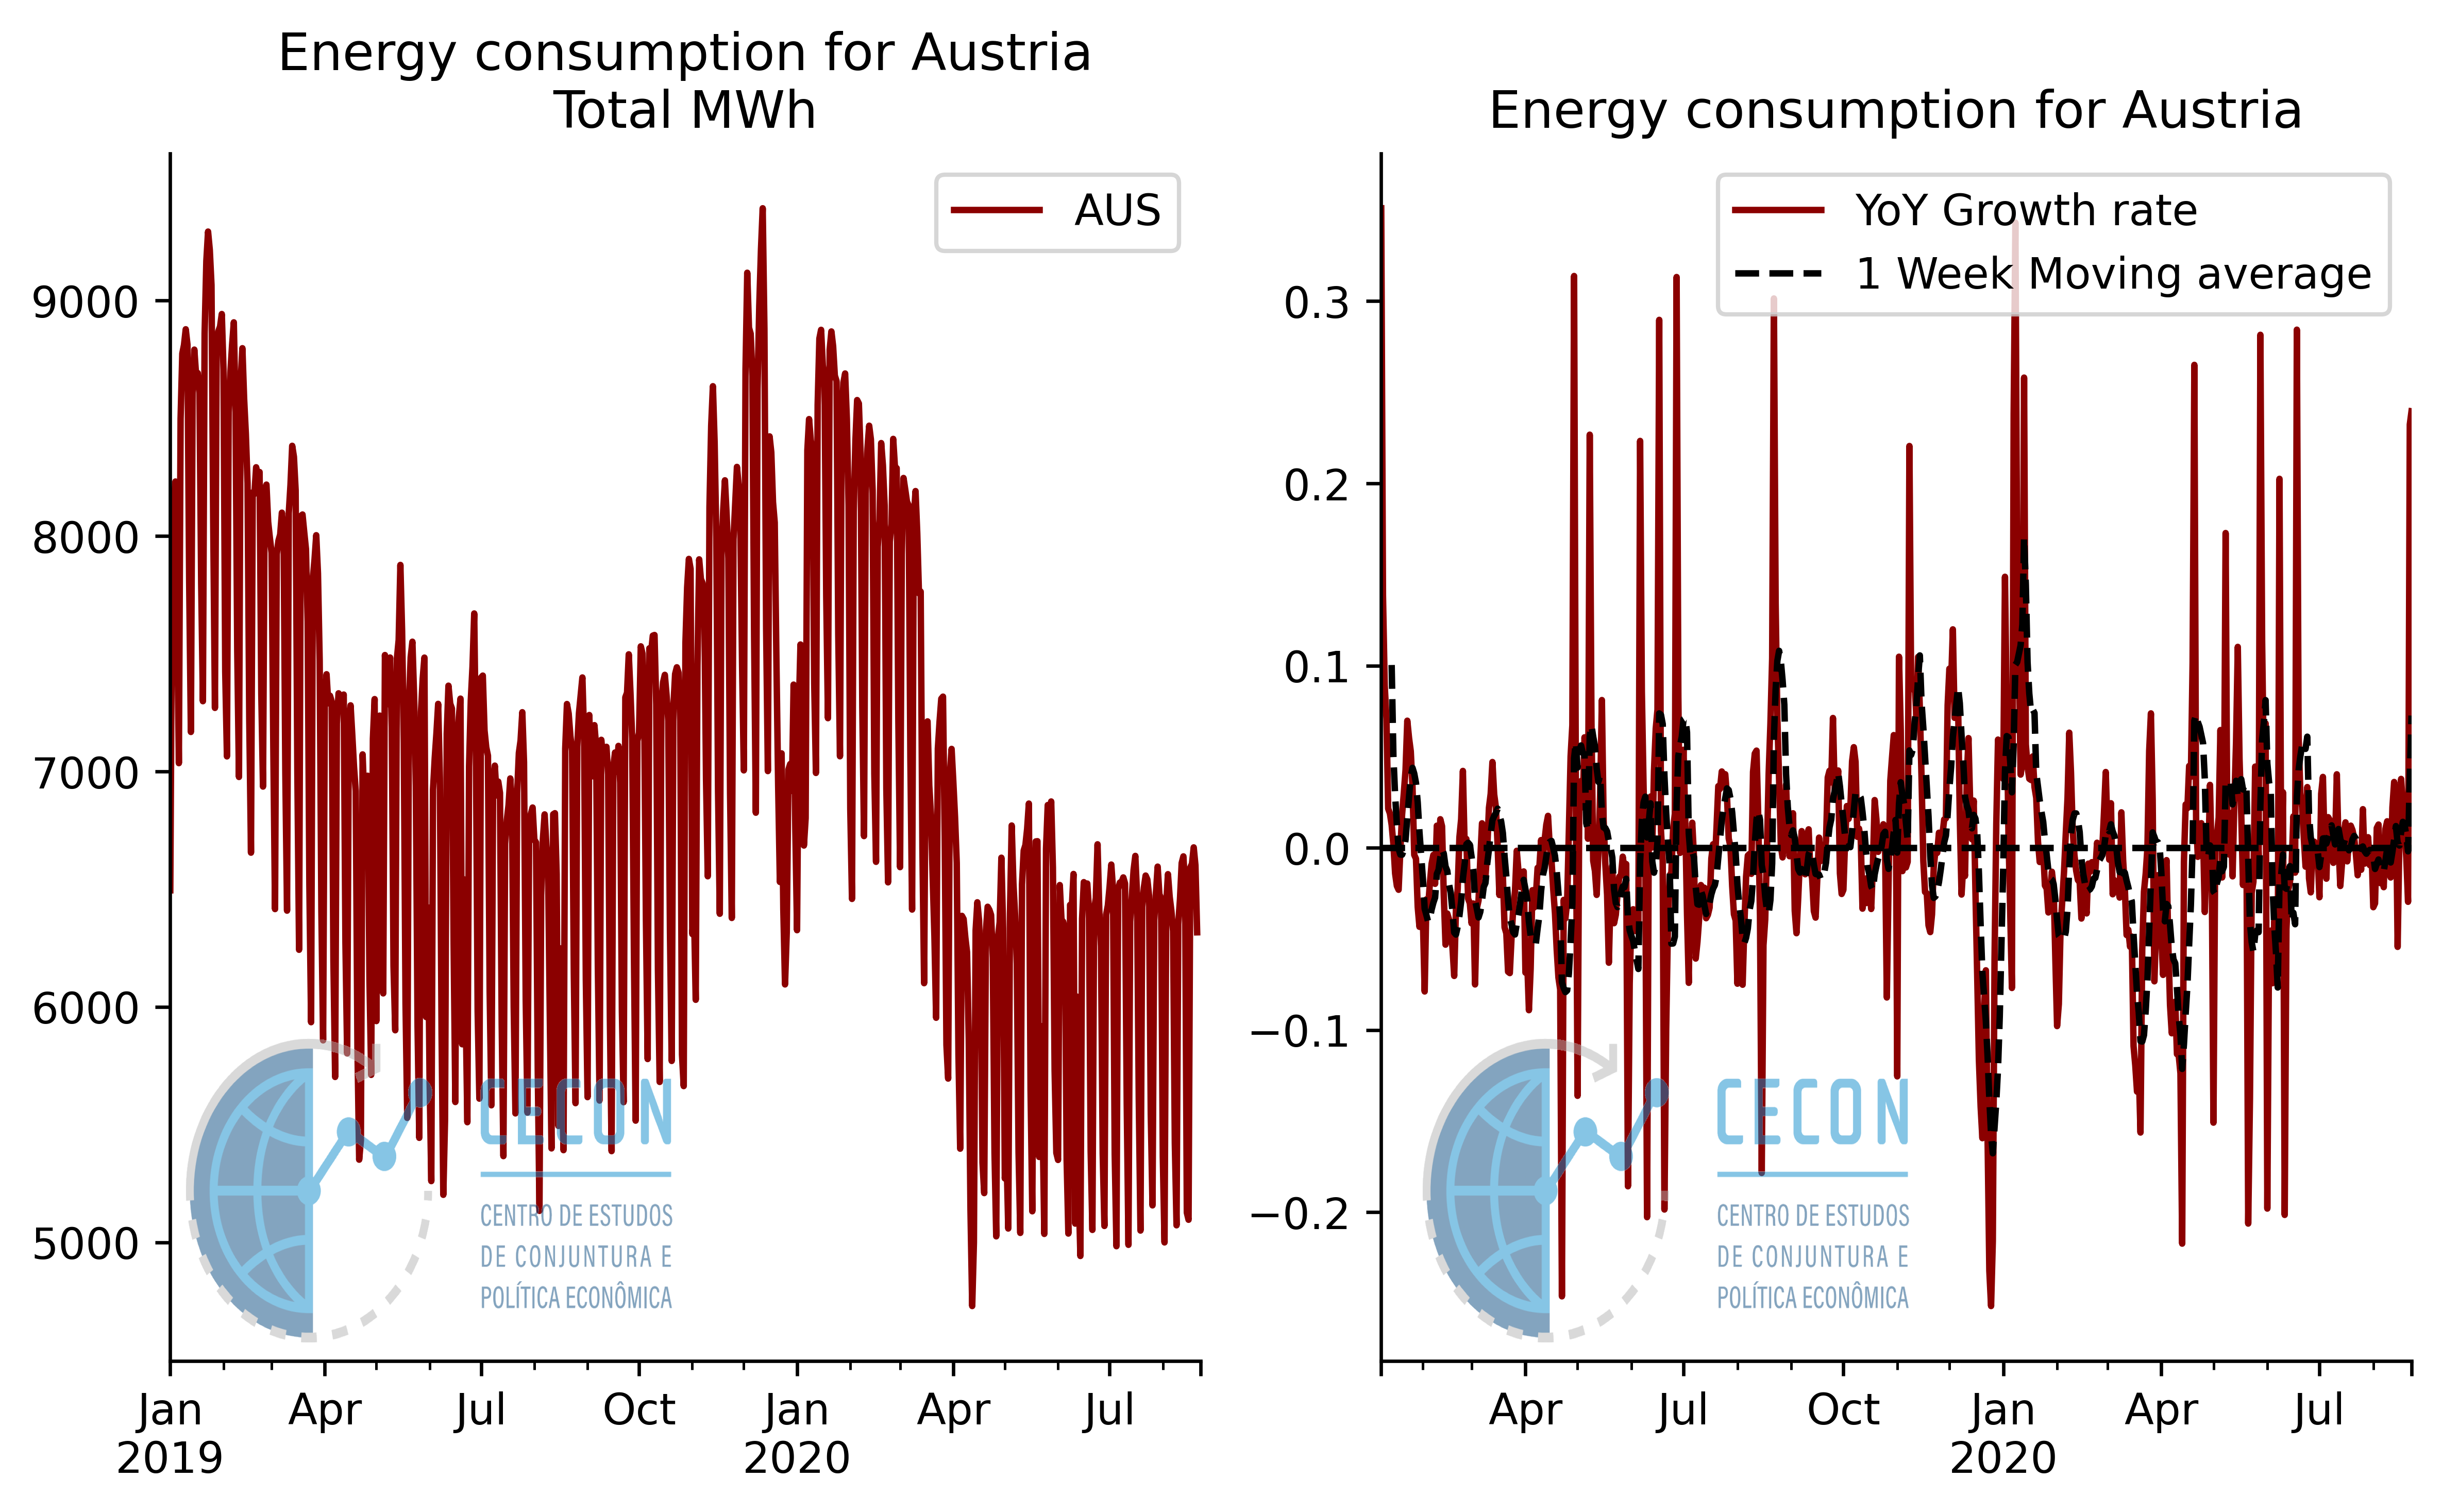
\includegraphics[width=.9\linewidth]{obipy-resources/62e383af79e91b63c7fc98dd7fb55b3c3ececcb9/9ef112a5872cc34e81a6bb8ef5d1a8c7b5fddf8e.png}
\end{center}

\subsubsection{Germany: GER}
\label{sec:org43bc300}

<ipython-input-21-06392b792fc4>:74: UserWarning: This figure includes Axes that are not compatible with tight\_layout, so results might be incorrect.
  plt.tight\_layout()

\begin{verbatim}
<Figure size 2400x1500 with 4 Axes>
\end{verbatim}


\begin{center}
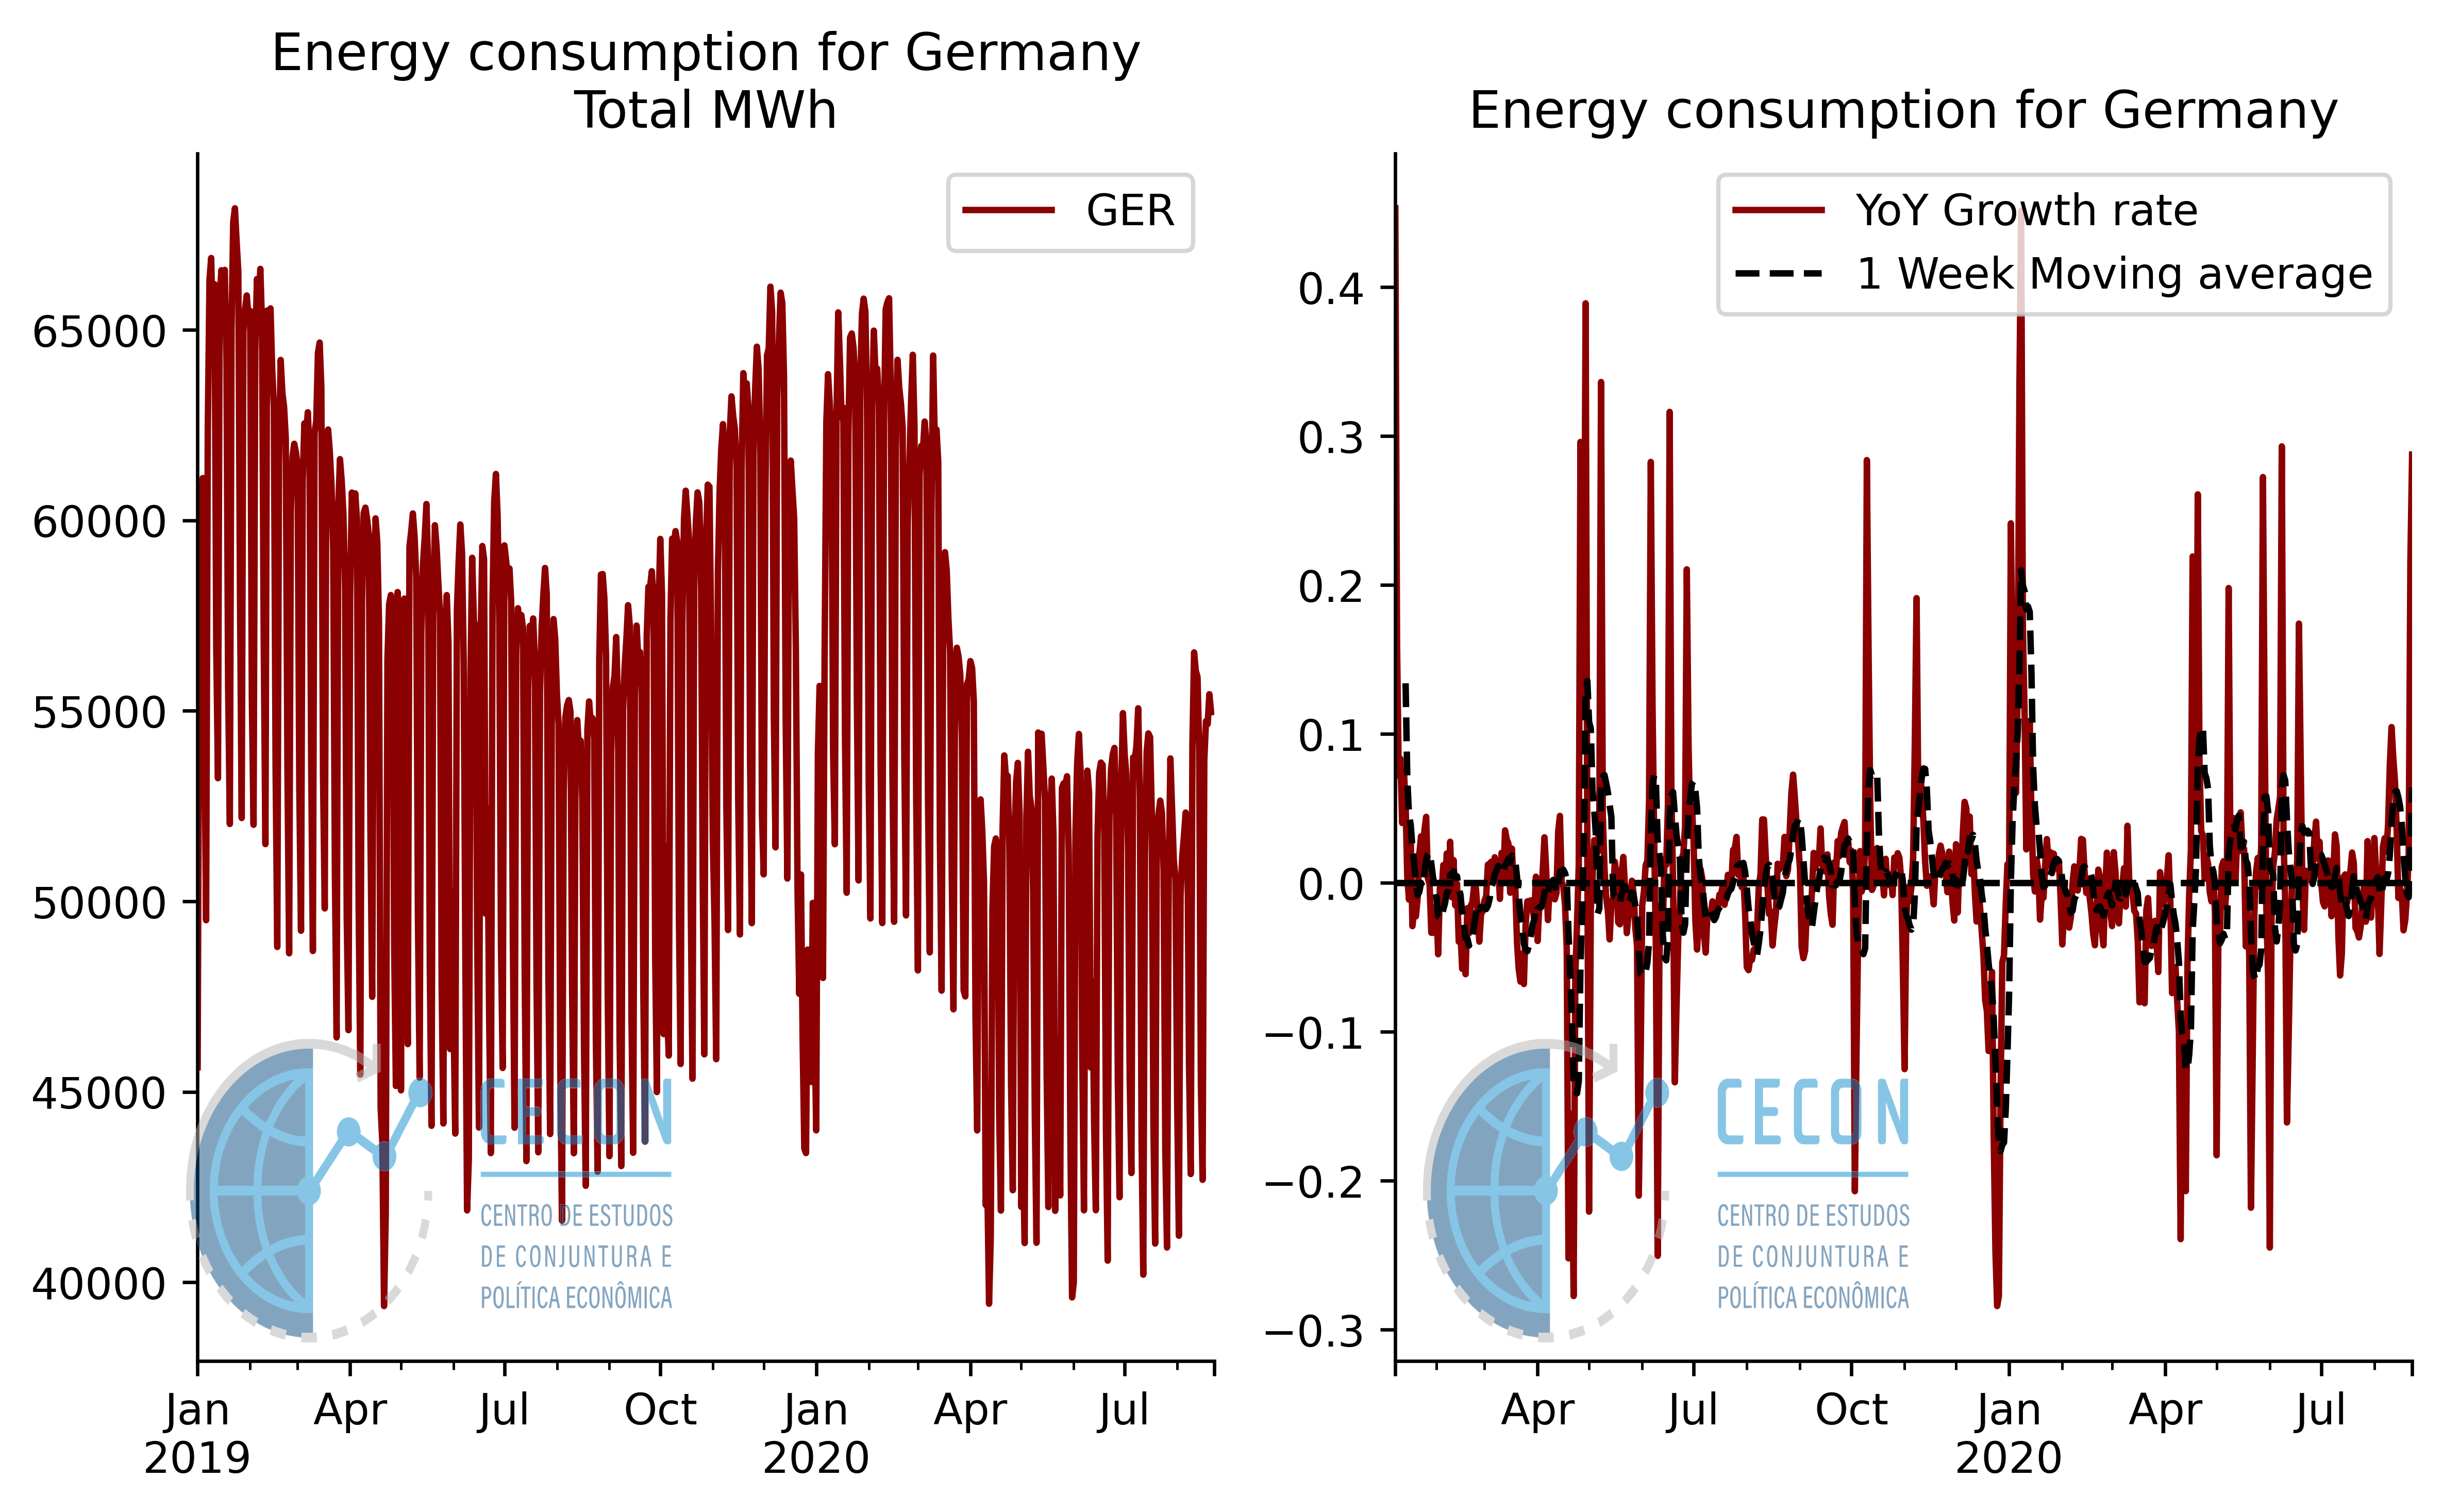
\includegraphics[width=.9\linewidth]{obipy-resources/62e383af79e91b63c7fc98dd7fb55b3c3ececcb9/94b114813ade8f5d4312e2e75f5b997a956c4a44.png}
\end{center}

\subsubsection{Luxemburg: LUX}
\label{sec:orgcff1ec7}

<ipython-input-21-06392b792fc4>:74: UserWarning: This figure includes Axes that are not compatible with tight\_layout, so results might be incorrect.
  plt.tight\_layout()

\begin{verbatim}
                   LUX
                      
2019-01-01  395.145833
2019-01-02  113.833333
2019-01-03    0.000000
2019-01-04  122.604167
2019-01-05  366.916667
...                ...
2020-08-19  395.208333
2020-08-20  476.333333
2020-08-21  414.705882
2020-08-22         NaN
2020-08-23         NaN

[601 rows x 1 columns]
\end{verbatim}


\url{file:///tmp/ob-ipython-html5ql3zW.html}

\begin{verbatim}
<Figure size 2400x1500 with 4 Axes>
\end{verbatim}


\begin{center}
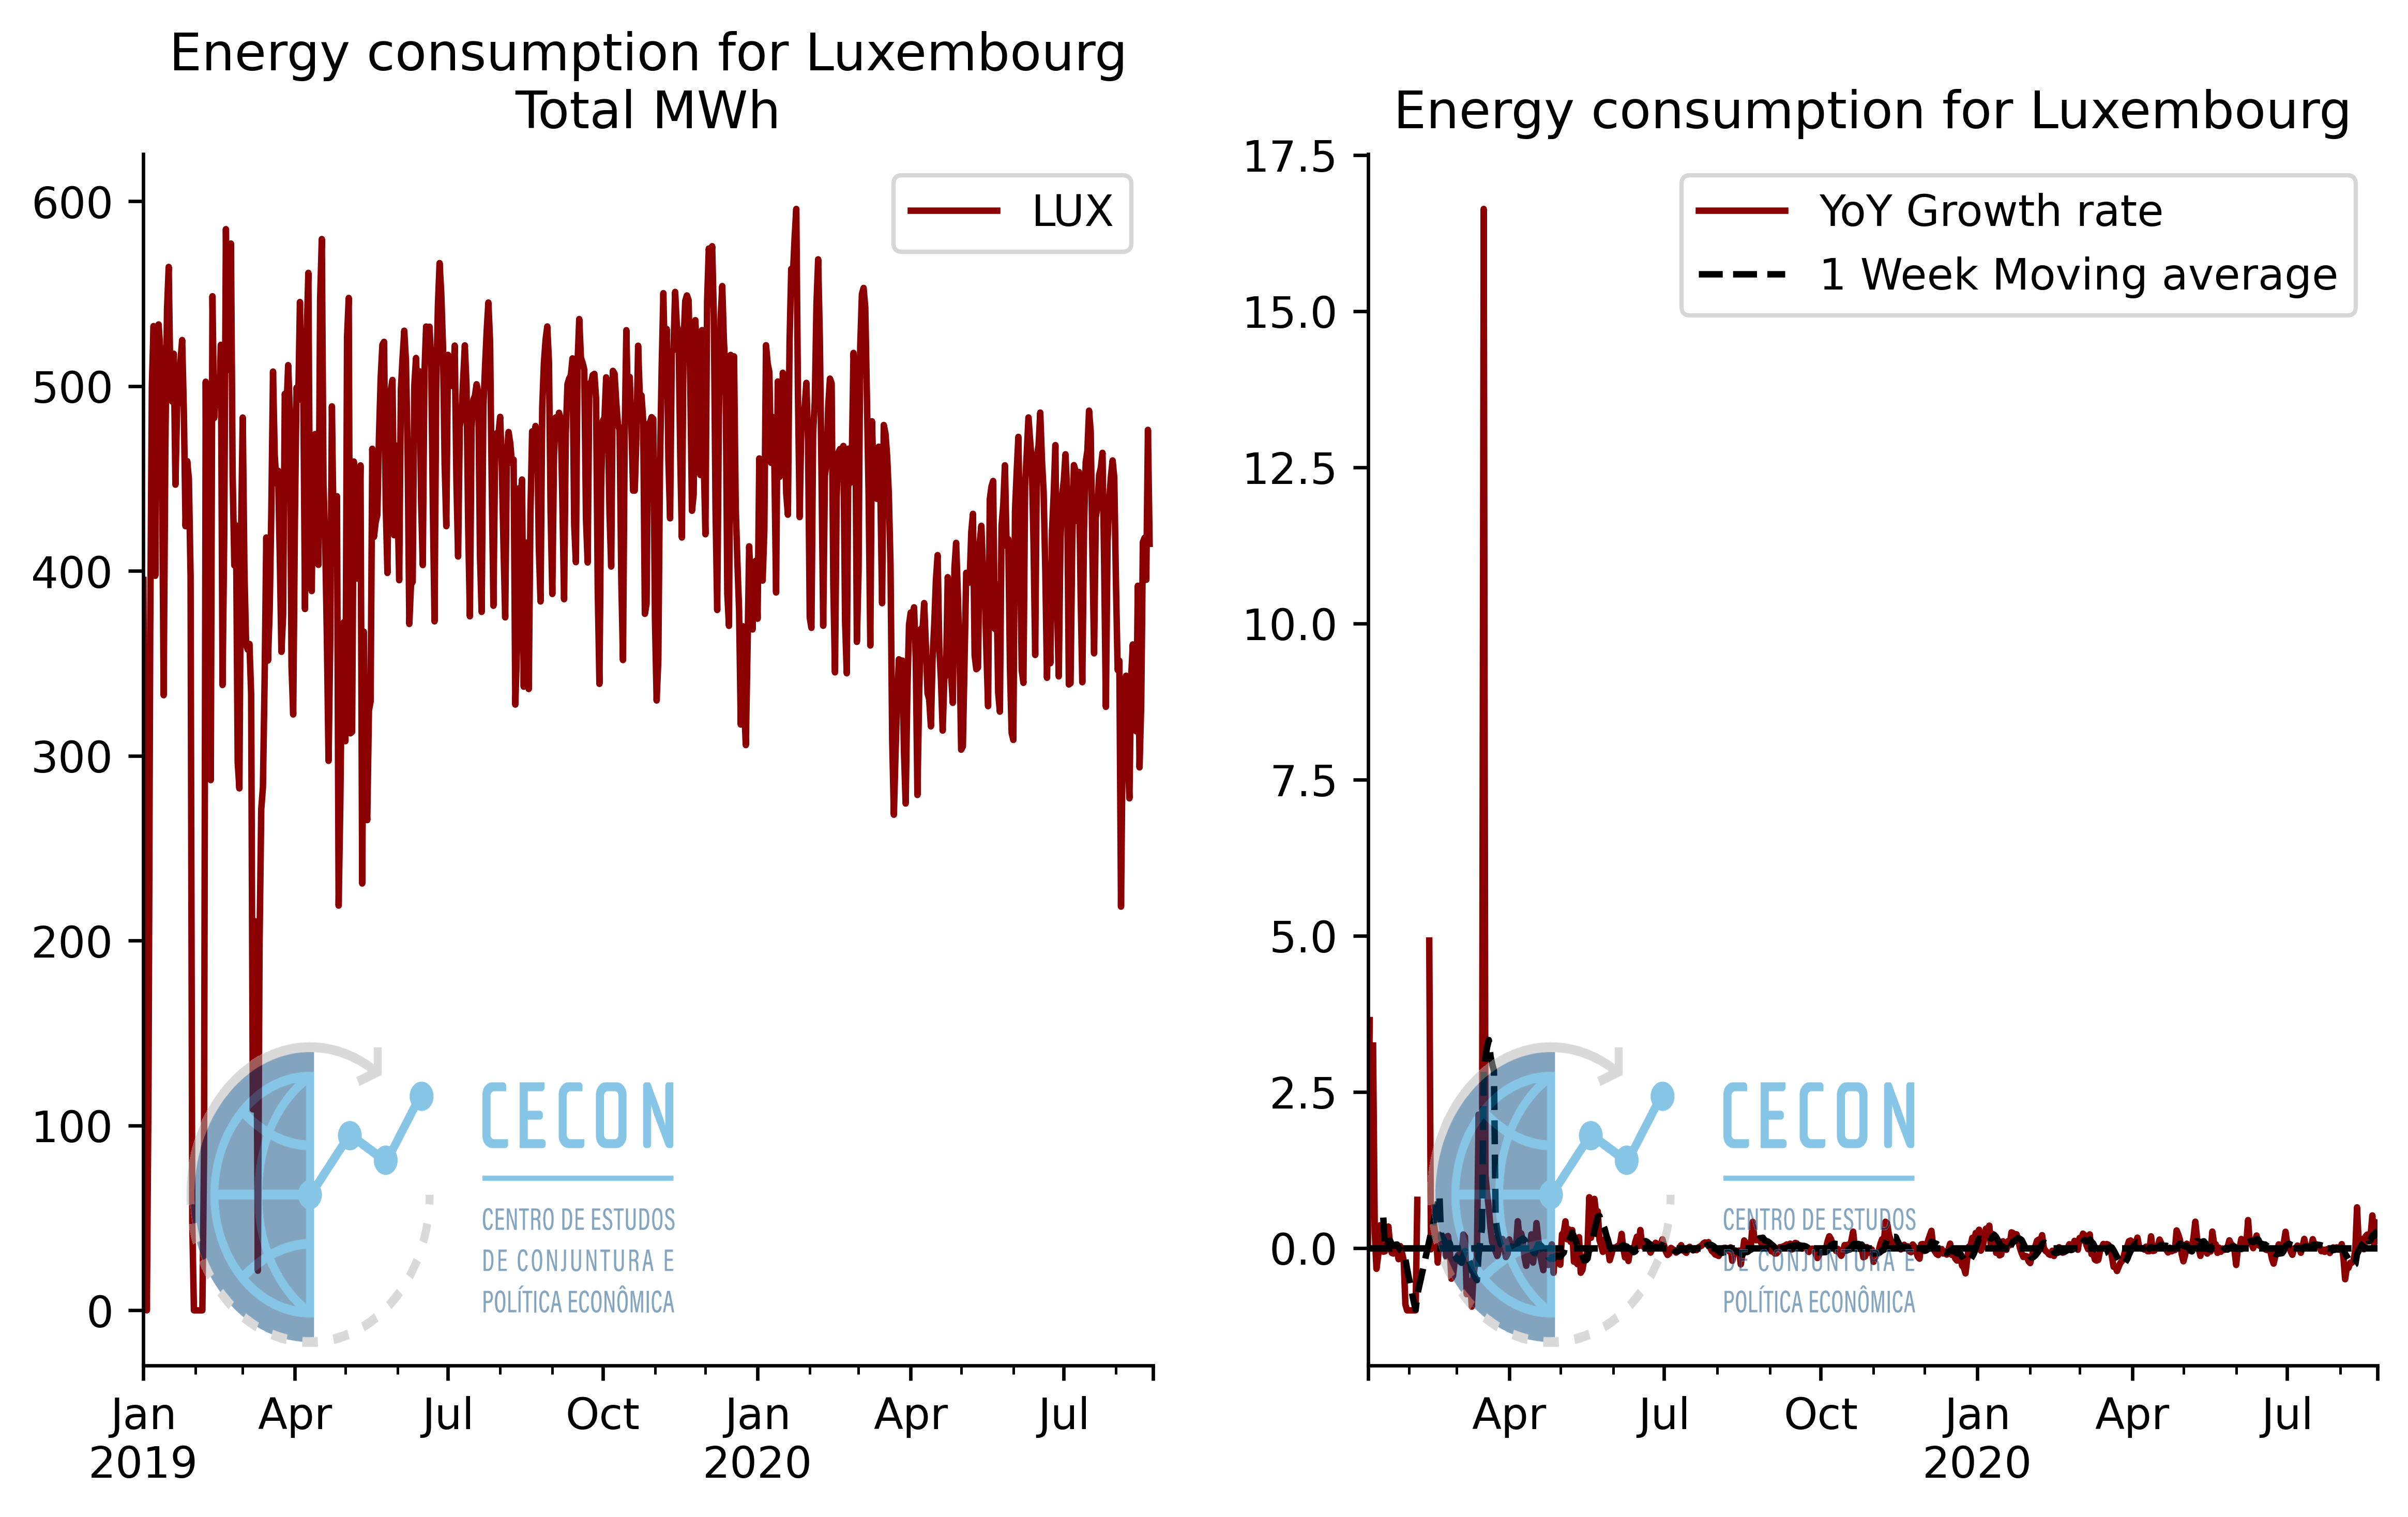
\includegraphics[width=.9\linewidth]{obipy-resources/62e383af79e91b63c7fc98dd7fb55b3c3ececcb9/9106e308f42f1f76c029539778f3952a7f562f15.png}
\end{center}


\subsection{Aruoba-Diebold-Scotti Business Conditions Index}
\label{sec:org6ef1419}

\begin{verbatim}
<Figure size 2400x1500 with 2 Axes>
\end{verbatim}


\begin{center}
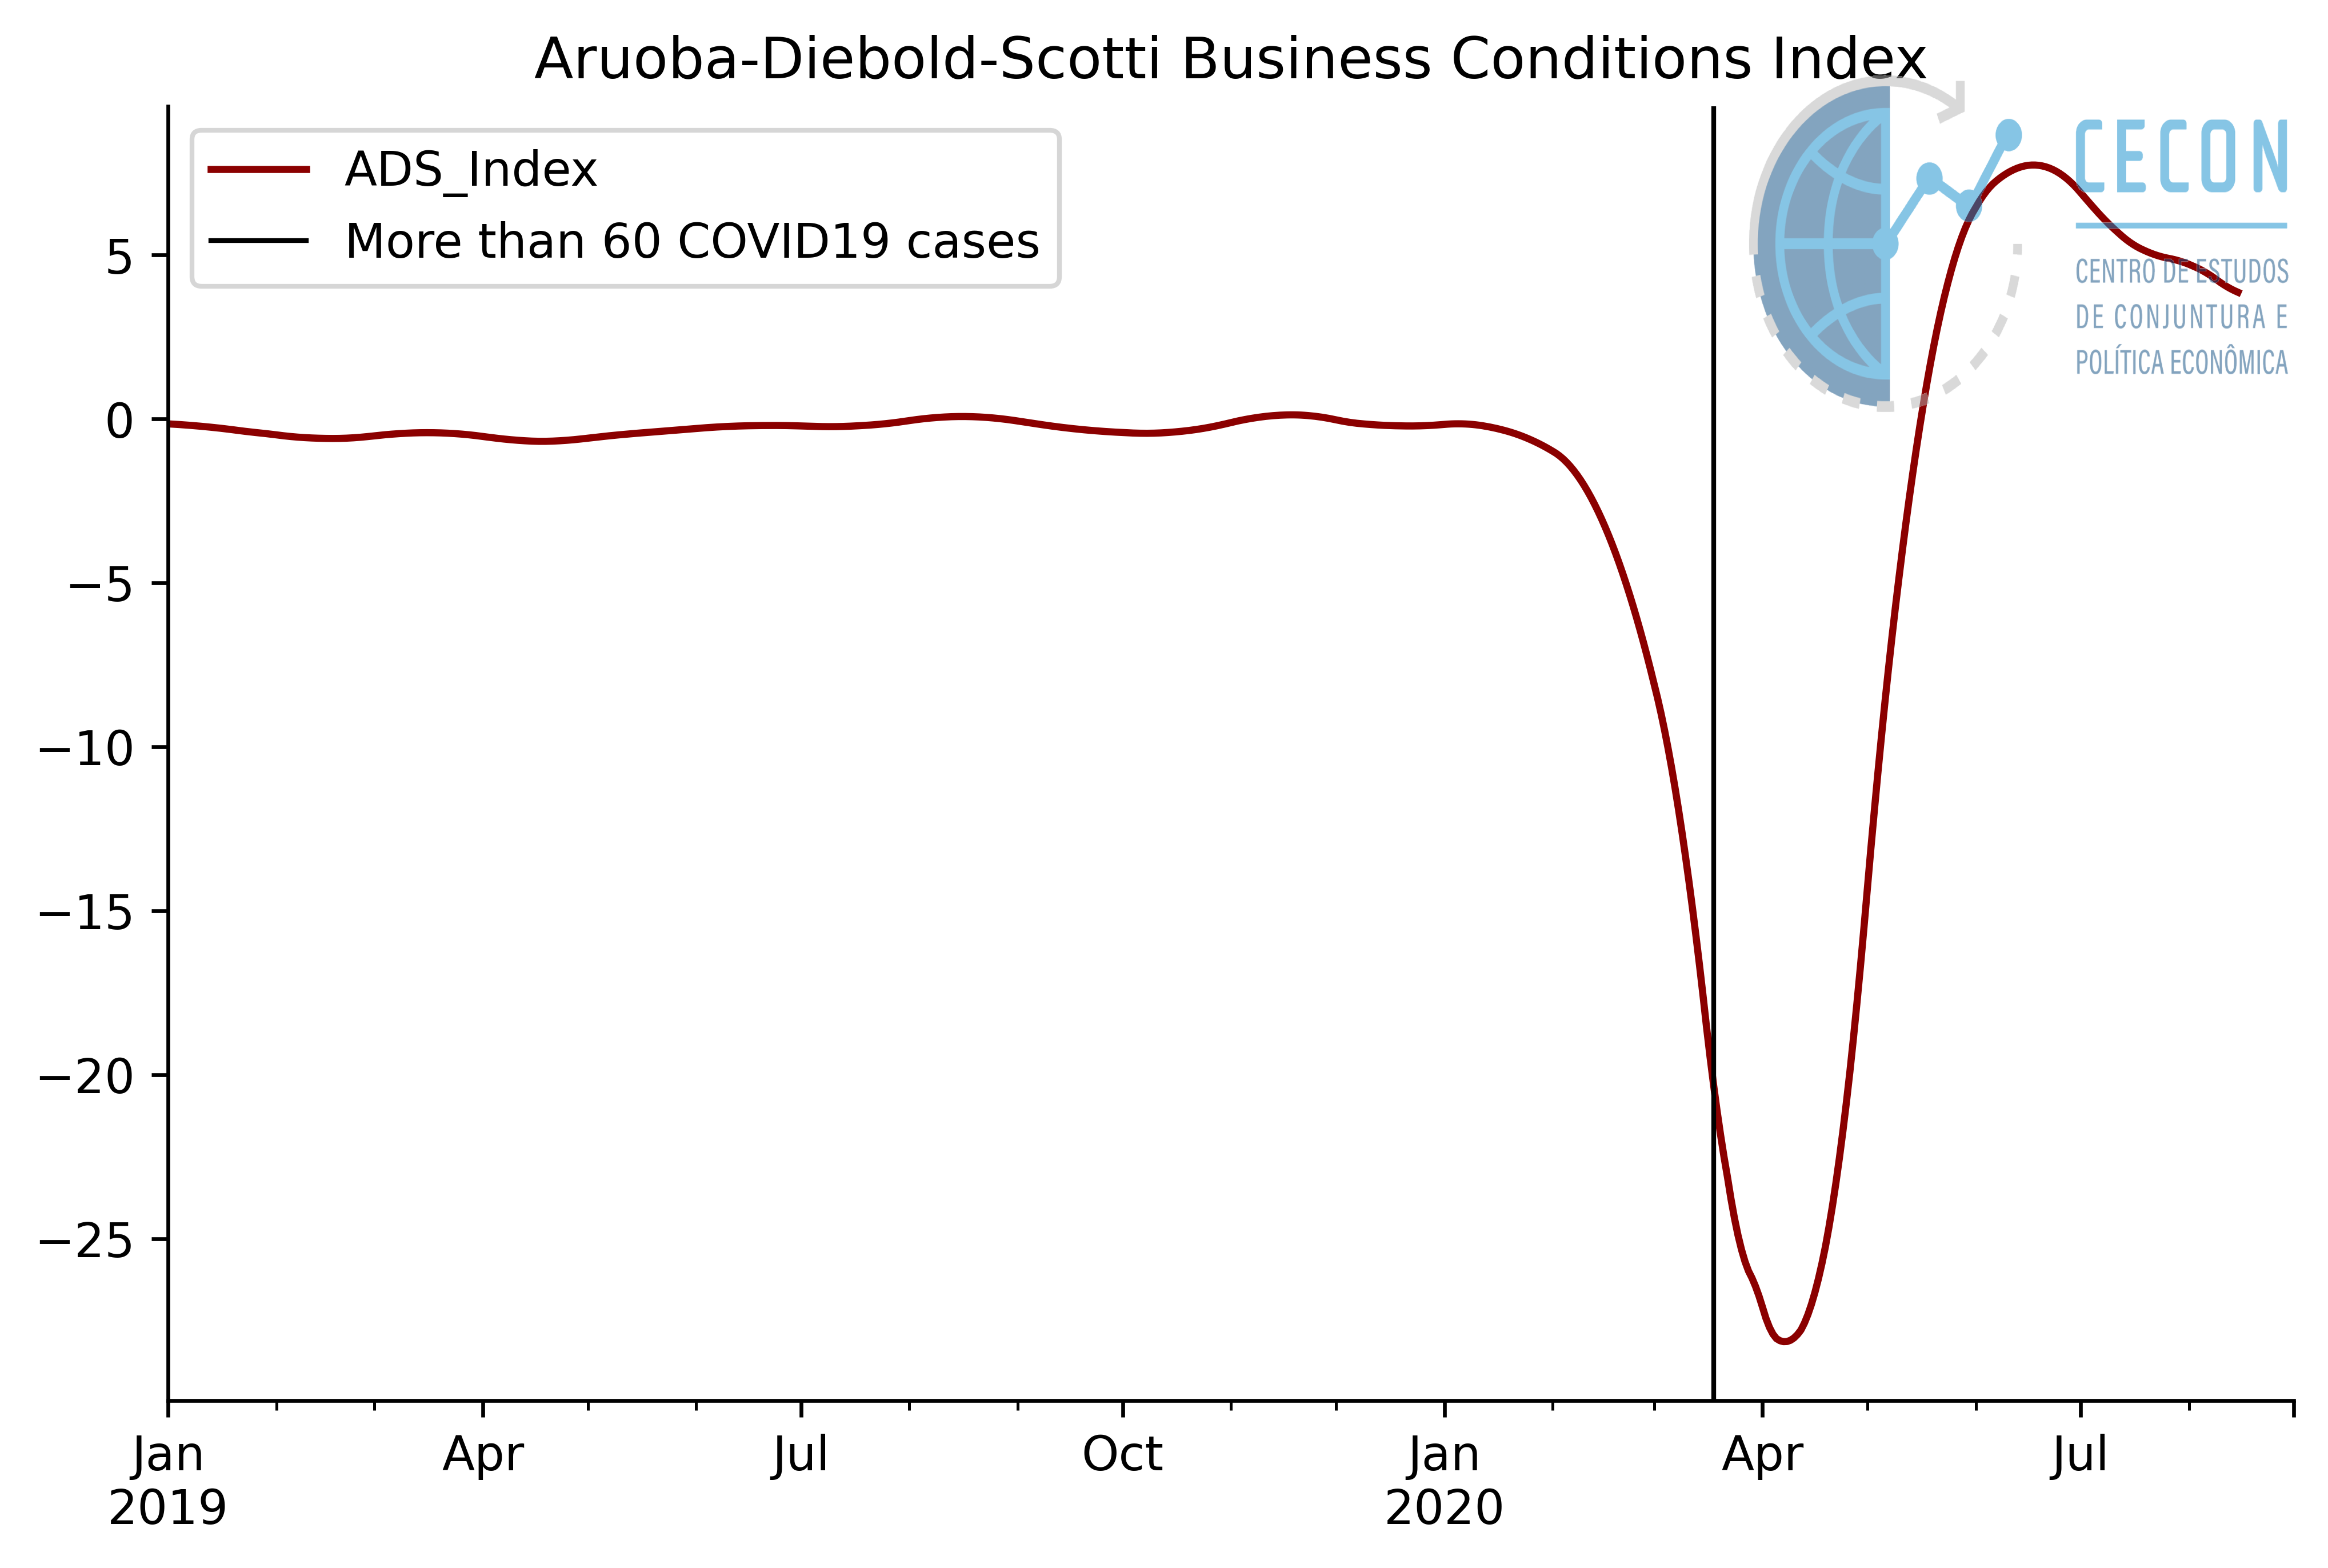
\includegraphics[width=.9\linewidth]{obipy-resources/62e383af79e91b63c7fc98dd7fb55b3c3ececcb9/cf14fa691a64e7d5e47f44565dc9f5363854ad6e.png}
\end{center}

\section{Confiança, Indicadores de antecedentes e de Risco}
\label{sec:org08c204f}

\subsection{Confiança}
\label{sec:org332f2f3}


\subsubsection{Sondagem Conjuntural Mensal}
\label{sec:org21ac13d}

\begin{verbatim}
<Figure size 576x360 with 2 Axes>
\end{verbatim}


\begin{center}
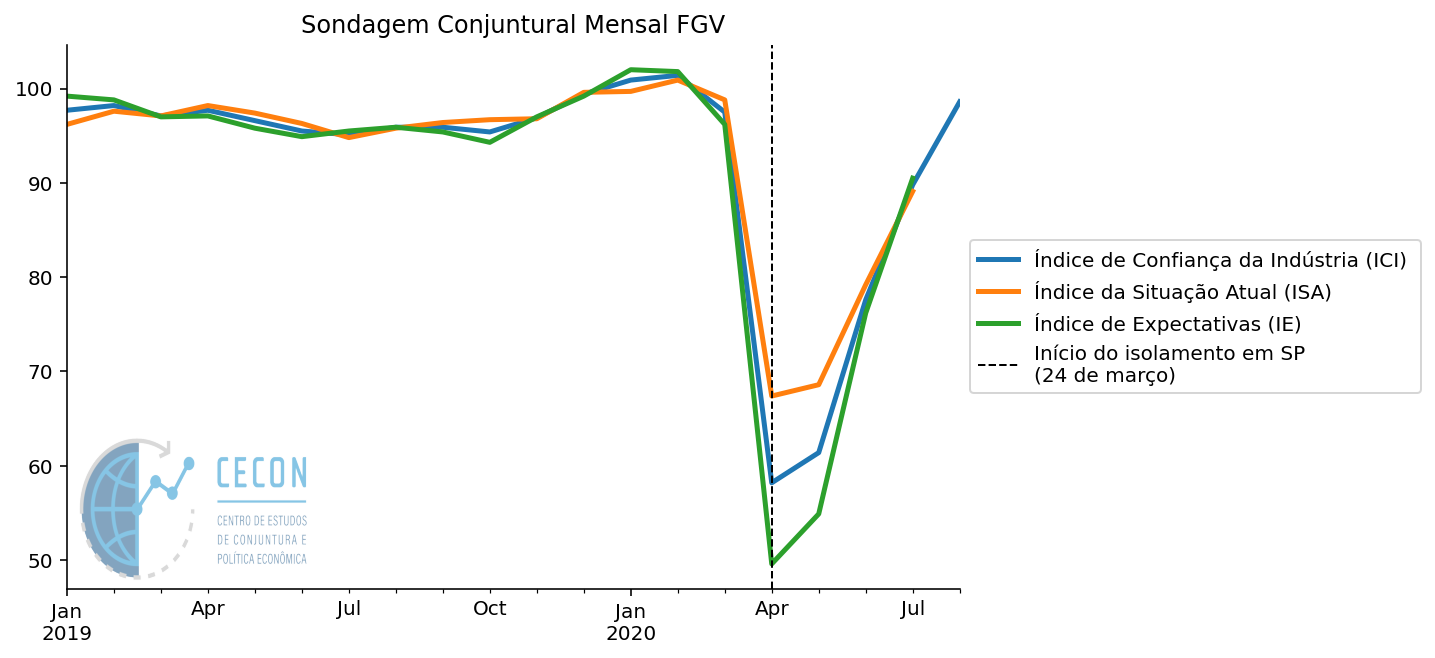
\includegraphics[width=.9\linewidth]{obipy-resources/62e383af79e91b63c7fc98dd7fb55b3c3ececcb9/7b3e58a37abae00e5e3eb5c1240536addcb36229.png}
\end{center}

\subsubsection{Sondagens de serviços}
\label{sec:org439db94}

\begin{verbatim}
<Figure size 576x360 with 2 Axes>
\end{verbatim}


\begin{center}
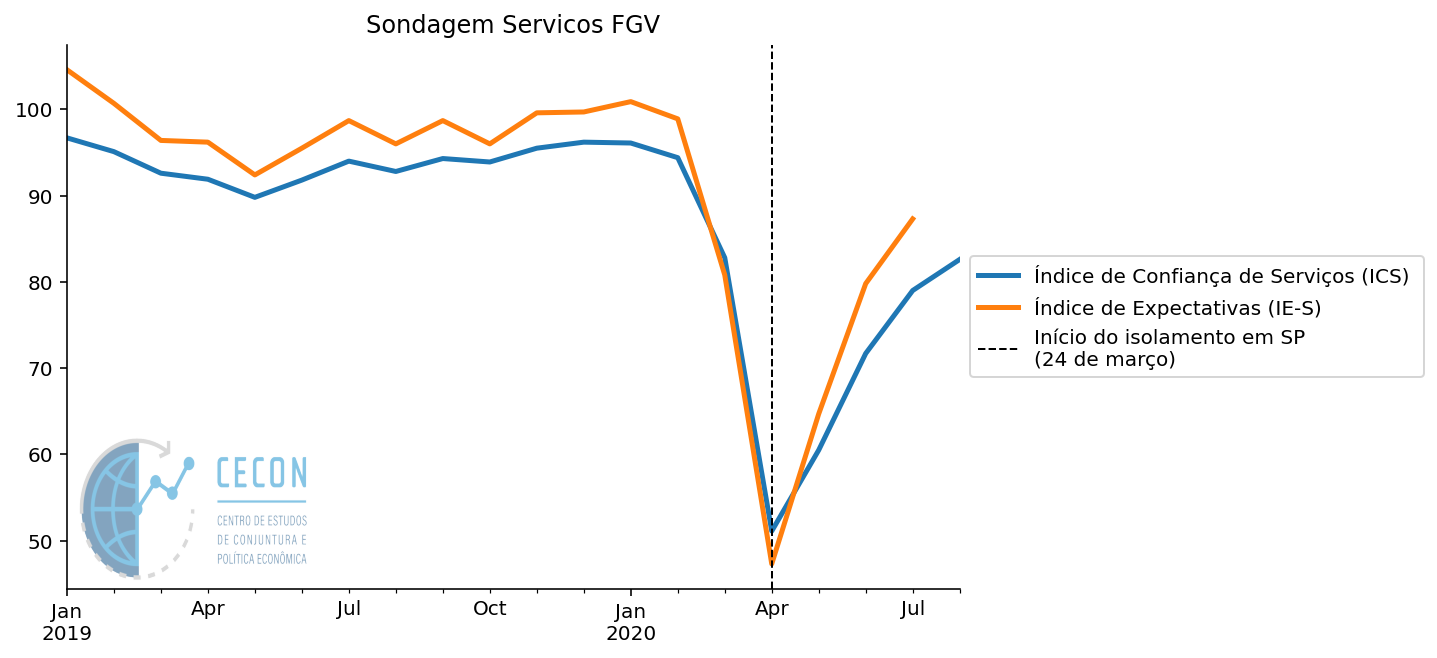
\includegraphics[width=.9\linewidth]{obipy-resources/62e383af79e91b63c7fc98dd7fb55b3c3ececcb9/aa0dc5316591c59e078ea9eb54ee5d1847c03529.png}
\end{center}


\subsubsection{Sondagem do comércio}
\label{sec:orgbc1fa86}

\begin{verbatim}
<Figure size 576x360 with 2 Axes>
\end{verbatim}


\begin{center}
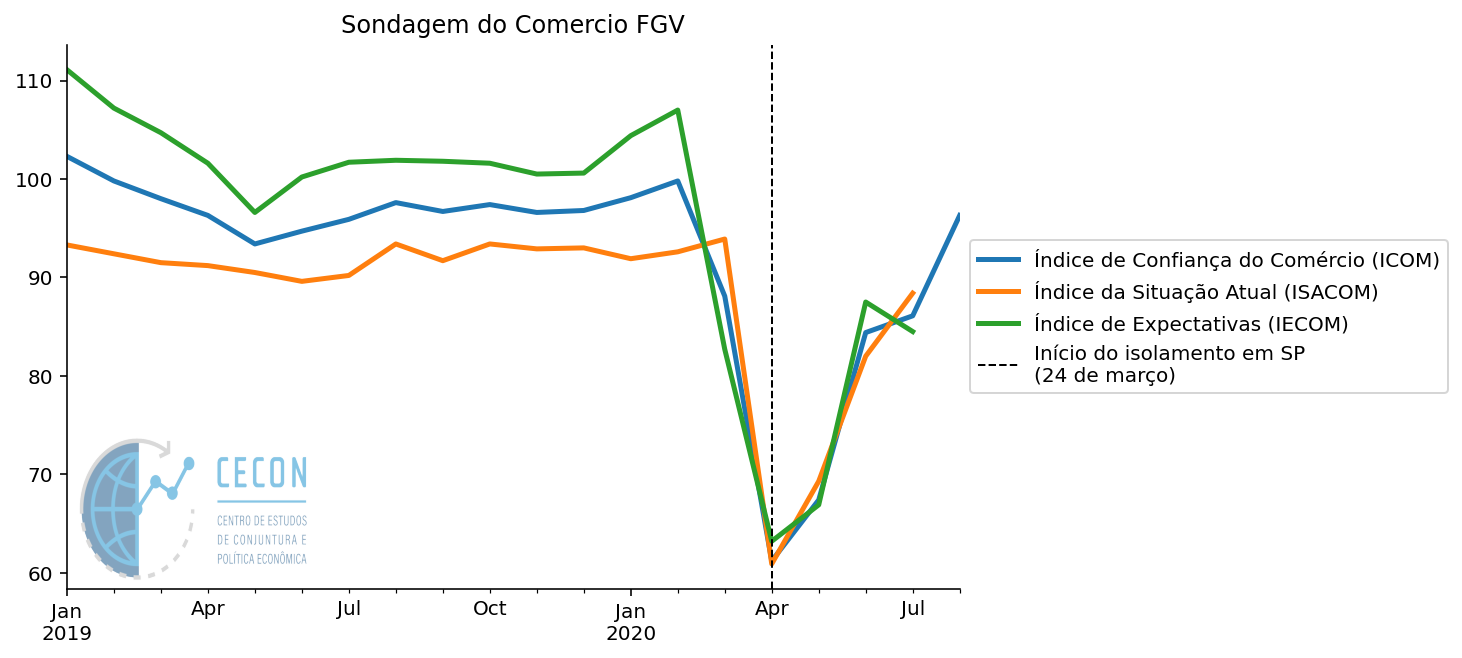
\includegraphics[width=.9\linewidth]{obipy-resources/62e383af79e91b63c7fc98dd7fb55b3c3ececcb9/554f61127530cd8c56d7d2bb715c64b18b66079b.png}
\end{center}

\subsubsection{Sondagem da construção}
\label{sec:orgb7aab35}

\begin{verbatim}
<Figure size 576x360 with 2 Axes>
\end{verbatim}


\begin{center}
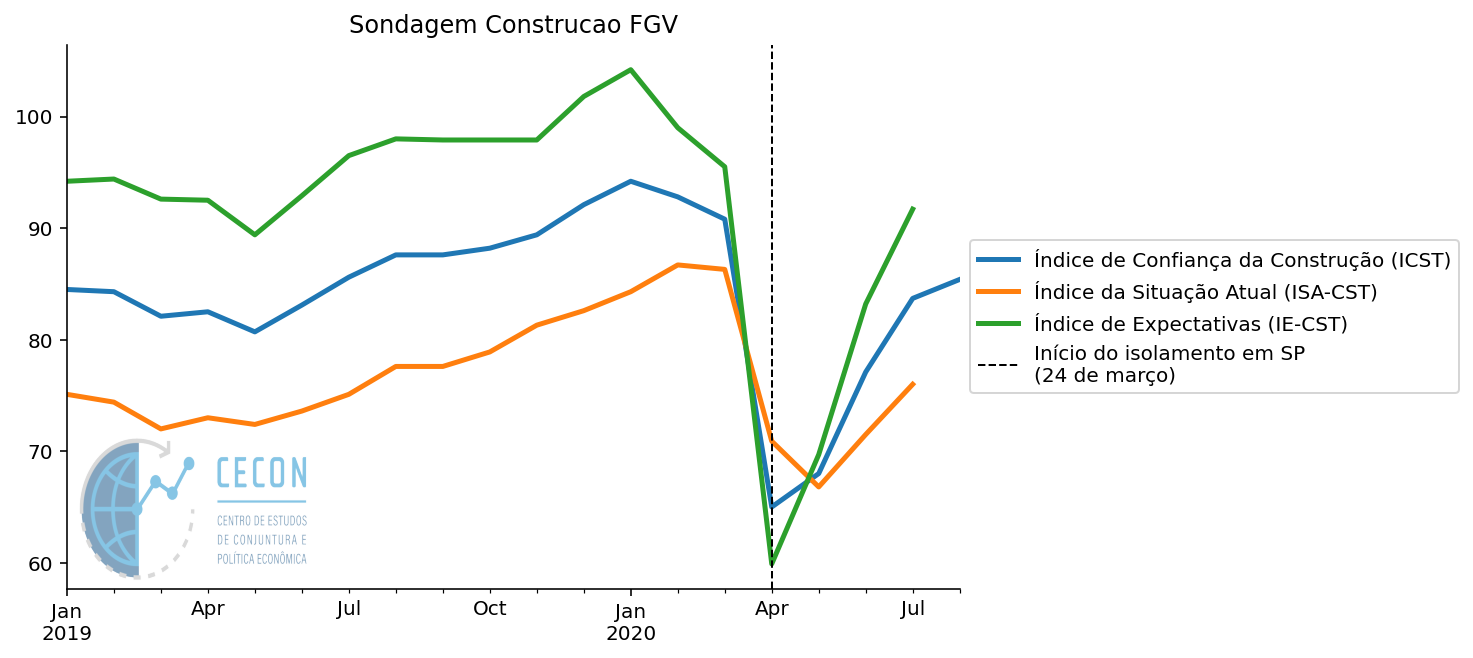
\includegraphics[width=.9\linewidth]{obipy-resources/62e383af79e91b63c7fc98dd7fb55b3c3ececcb9/5c55149be31444f847711890239c1aa99b605e4e.png}
\end{center}

\subsubsection{Sondagem industrial CNI}
\label{sec:orgbbf3a96}


\begin{enumerate}
\item Volume de produção
\label{sec:org6af0afa}

\begin{verbatim}
<Figure size 576x360 with 2 Axes>
\end{verbatim}


\begin{center}
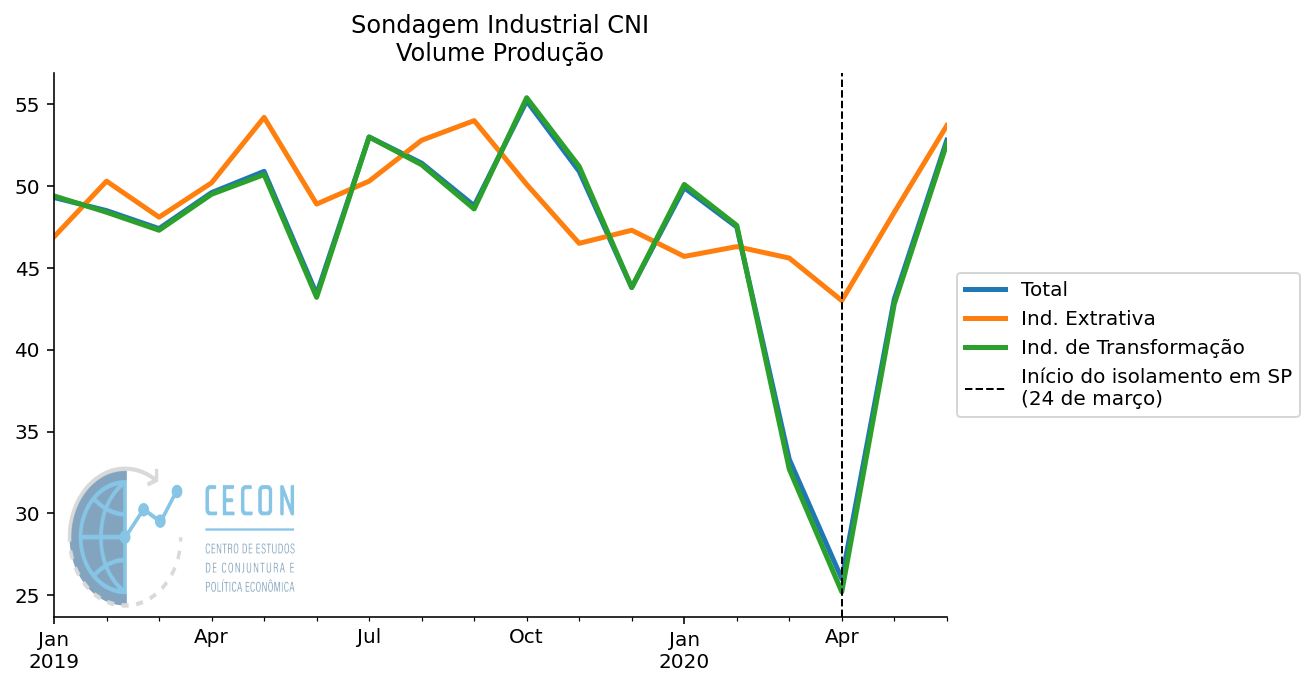
\includegraphics[width=.9\linewidth]{obipy-resources/62e383af79e91b63c7fc98dd7fb55b3c3ececcb9/38f547e28e64d3a45c6d27a727a62aa301d80753.png}
\end{center}

\item Evolução do Emprego
\label{sec:orgaa8647c}

\begin{verbatim}
<Figure size 576x360 with 2 Axes>
\end{verbatim}


\begin{center}
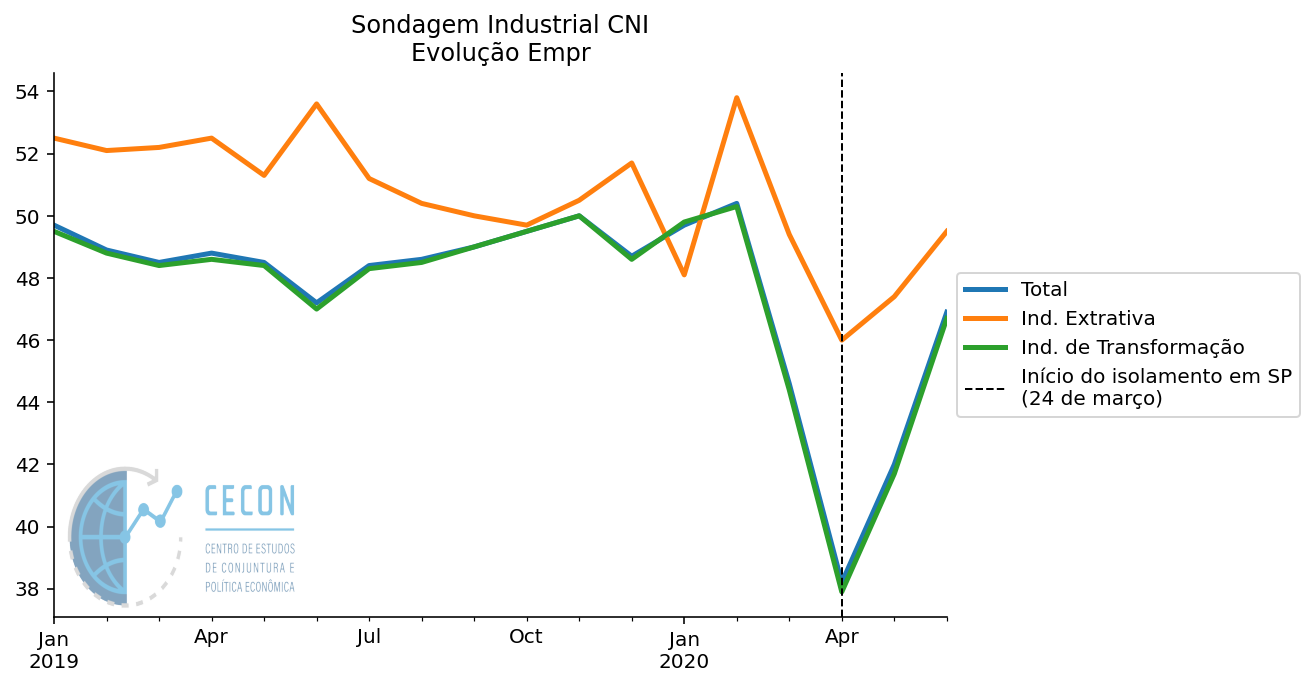
\includegraphics[width=.9\linewidth]{obipy-resources/62e383af79e91b63c7fc98dd7fb55b3c3ececcb9/f37059e5663a6183f7323a2bea6f3b8ed9dba88f.png}
\end{center}


\item NUCI
\label{sec:orgf65db06}

\begin{verbatim}
<Figure size 576x360 with 2 Axes>
\end{verbatim}


\begin{center}
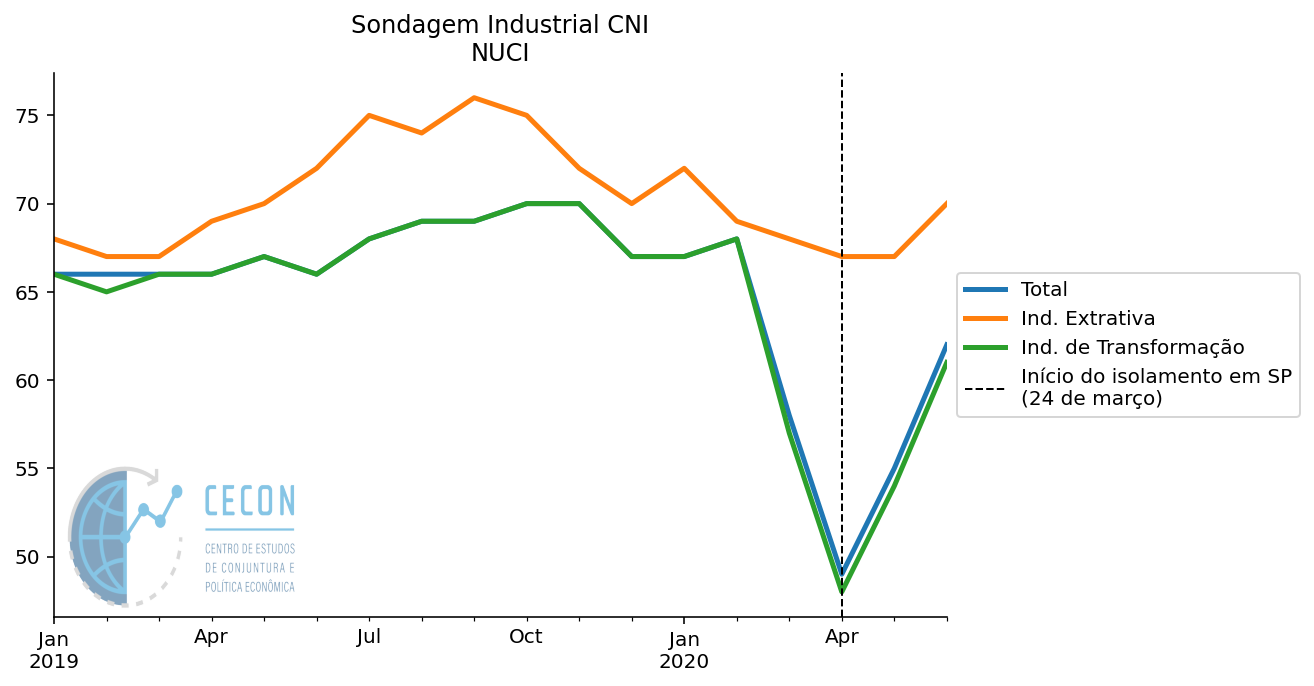
\includegraphics[width=.9\linewidth]{obipy-resources/62e383af79e91b63c7fc98dd7fb55b3c3ececcb9/168c9d12b41c7ac07608ad8d75414f133fd99cf6.png}
\end{center}

\item NUCI Efeito-Usual
\label{sec:org912e02d}

\begin{verbatim}
<Figure size 576x360 with 2 Axes>
\end{verbatim}


\begin{center}
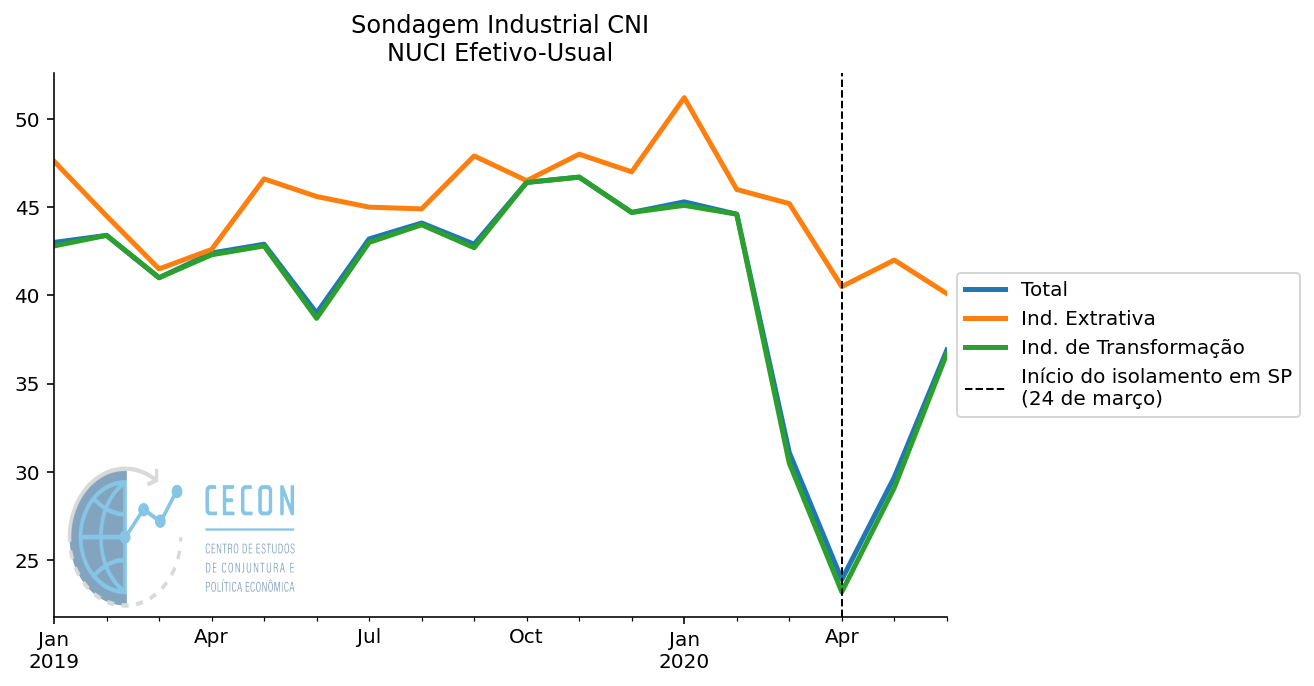
\includegraphics[width=.9\linewidth]{obipy-resources/62e383af79e91b63c7fc98dd7fb55b3c3ececcb9/7a0bc786fc2b366f513e486fa9da04f995e06c54.png}
\end{center}

\item Evolução de estoques
\label{sec:org51cc43d}

\begin{verbatim}
<Figure size 576x360 with 2 Axes>
\end{verbatim}


\begin{center}
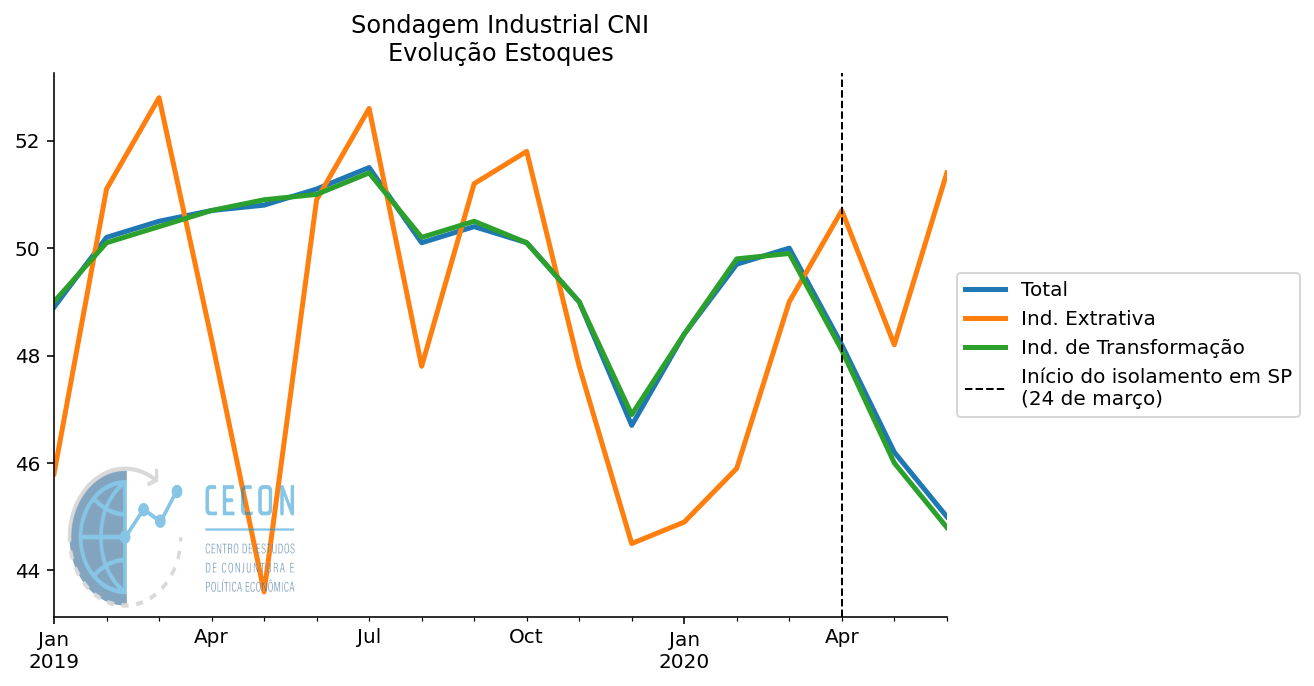
\includegraphics[width=.9\linewidth]{obipy-resources/62e383af79e91b63c7fc98dd7fb55b3c3ececcb9/fd32fd3f47edd7d6ff75dd215a315cbf0b037f86.png}
\end{center}

\item Estoques efetivos
\label{sec:orgee35636}

\begin{verbatim}
<Figure size 576x360 with 2 Axes>
\end{verbatim}


\begin{center}
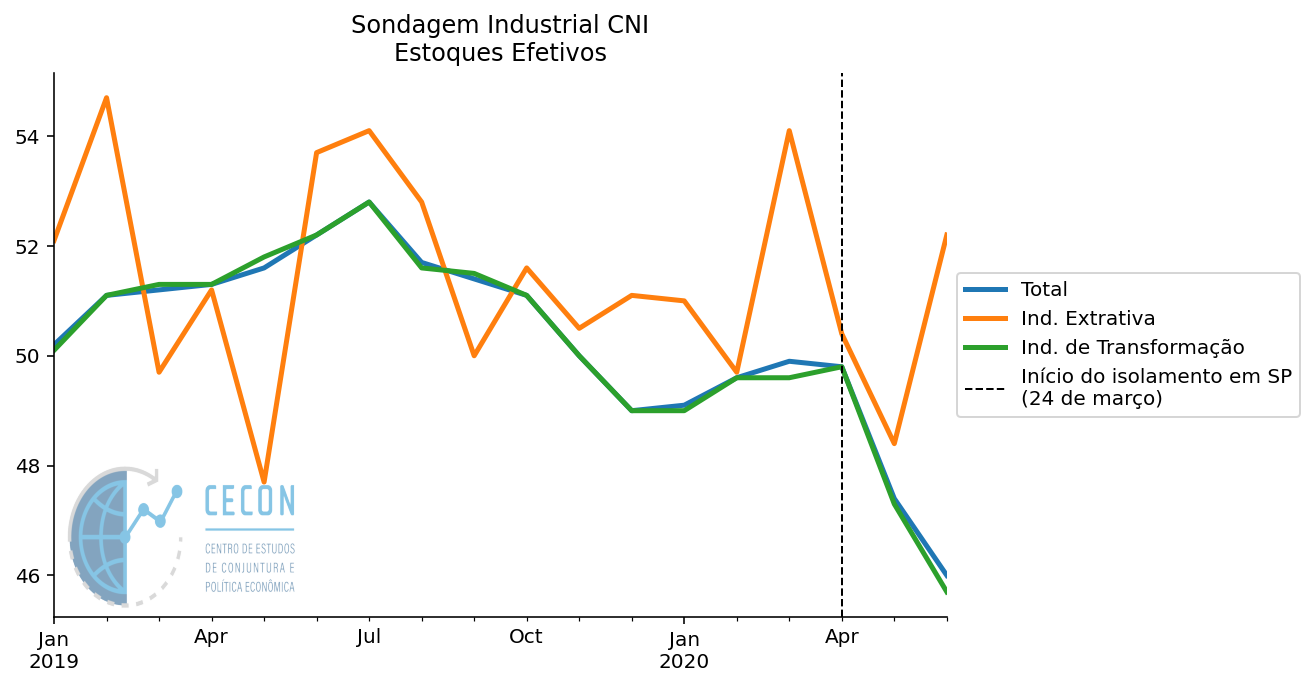
\includegraphics[width=.9\linewidth]{obipy-resources/62e383af79e91b63c7fc98dd7fb55b3c3ececcb9/1cd65f04161dcd94829a4e8d585f9e9c2038b23e.png}
\end{center}

\item Expectativa de Demanda
\label{sec:org4f3a63a}

\begin{verbatim}
<Figure size 576x360 with 2 Axes>
\end{verbatim}


\begin{center}
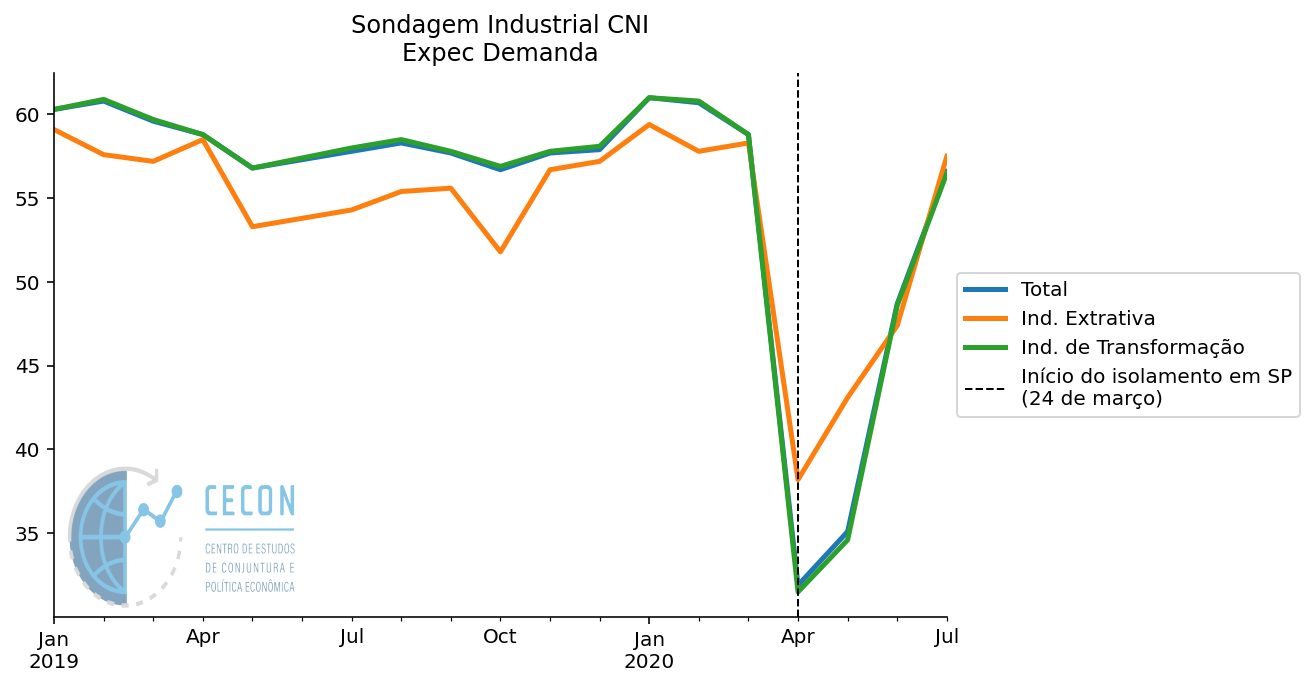
\includegraphics[width=.9\linewidth]{obipy-resources/62e383af79e91b63c7fc98dd7fb55b3c3ececcb9/d175d203a1e0fa24dab98a4cc430d67b312fc504.png}
\end{center}

\item Expectativa de Exportação
\label{sec:org3dfb3b5}

\begin{verbatim}
<Figure size 576x360 with 2 Axes>
\end{verbatim}


\begin{center}
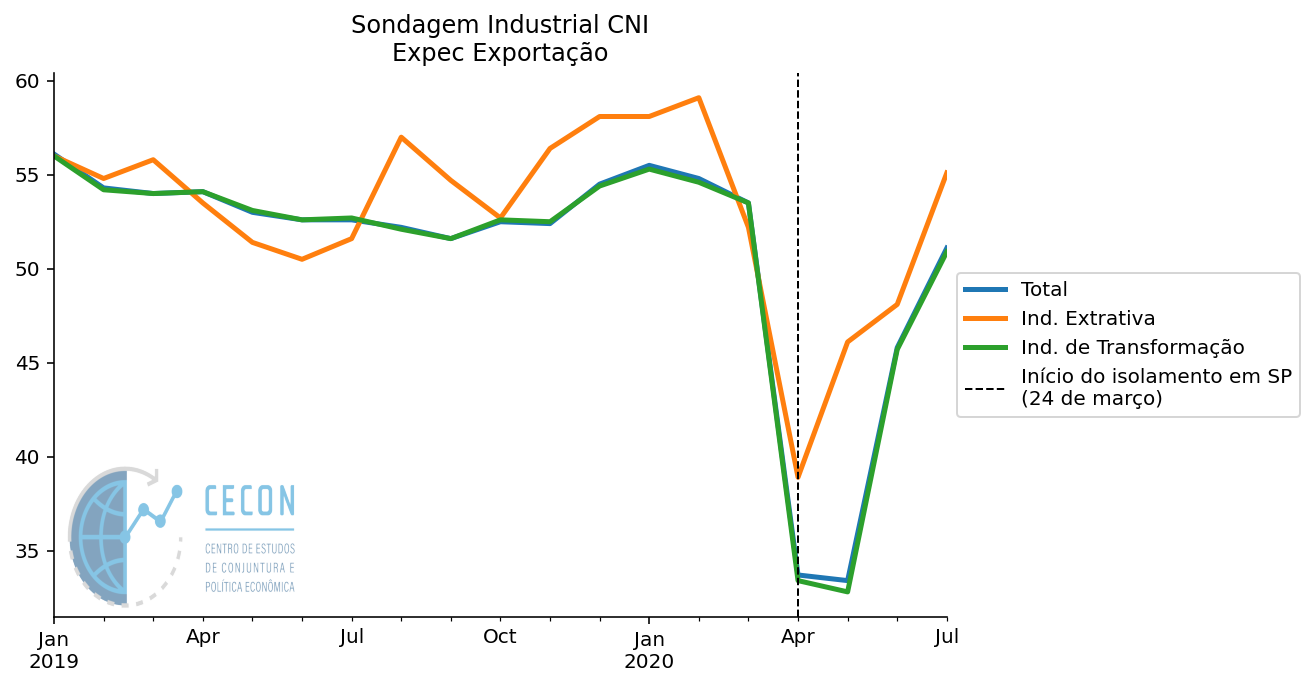
\includegraphics[width=.9\linewidth]{obipy-resources/62e383af79e91b63c7fc98dd7fb55b3c3ececcb9/9b4f75ae5dfbd3b780483f3ba4e18217227ba501.png}
\end{center}

\item Expectativa de compra de matéria-prima
\label{sec:orge0216de}


\begin{verbatim}
<Figure size 576x360 with 2 Axes>
\end{verbatim}


\begin{center}
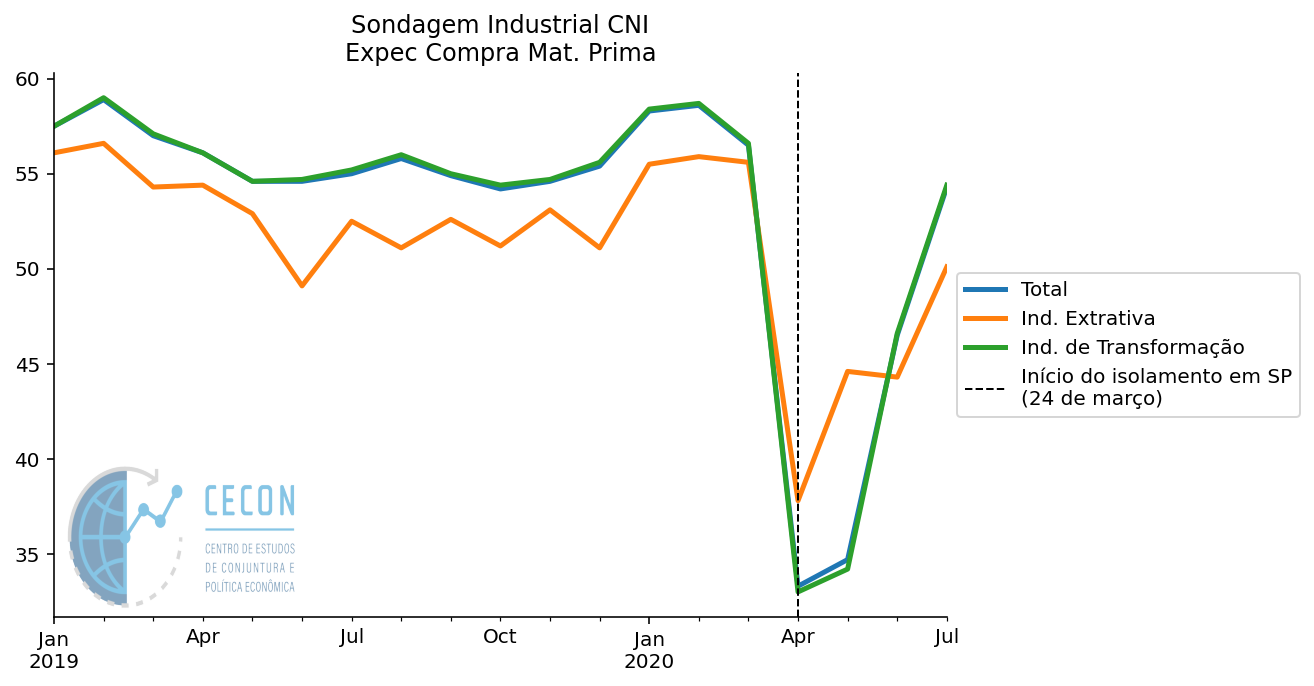
\includegraphics[width=.9\linewidth]{obipy-resources/62e383af79e91b63c7fc98dd7fb55b3c3ececcb9/cc12013aec1a7595bfa8d41ae3d6896fb2a84060.png}
\end{center}

\item Expectativa de emprego
\label{sec:orgec14f96}

\begin{verbatim}
<Figure size 576x360 with 2 Axes>
\end{verbatim}


\begin{center}
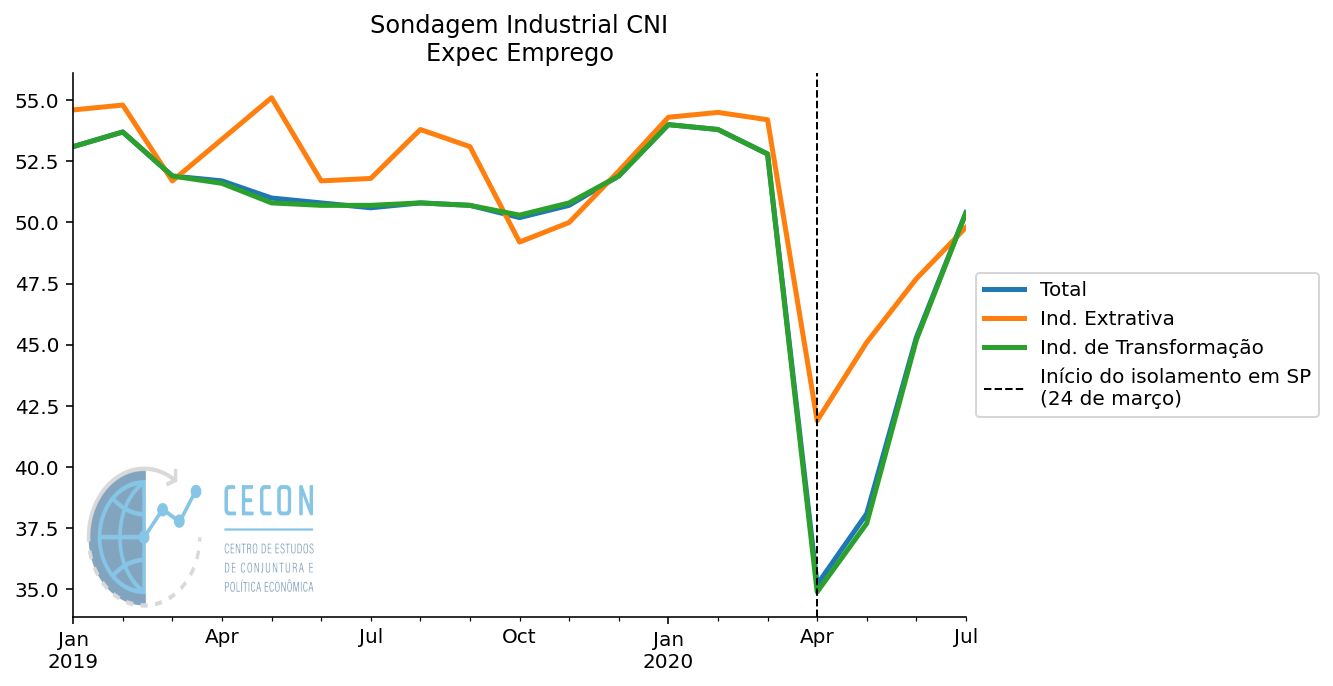
\includegraphics[width=.9\linewidth]{obipy-resources/62e383af79e91b63c7fc98dd7fb55b3c3ececcb9/8c83f58d6340a55e998ad231fb16037ce6828c59.png}
\end{center}

\item Expectativa de investimento
\label{sec:orgabe882b}

\begin{verbatim}
<Figure size 576x360 with 2 Axes>
\end{verbatim}


\begin{center}
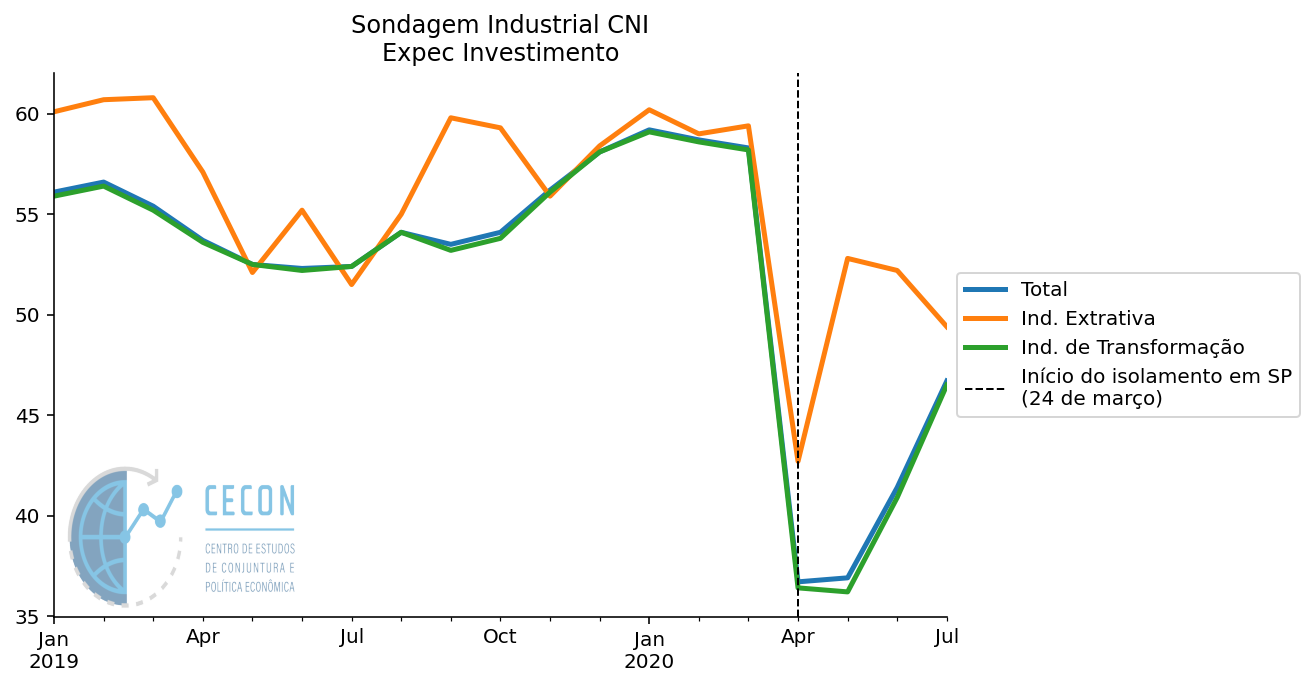
\includegraphics[width=.9\linewidth]{obipy-resources/62e383af79e91b63c7fc98dd7fb55b3c3ececcb9/b0bc7180843da18ade4ca5c8b9ba738f9a5ebd32.png}
\end{center}

\item Lucro Operacional
\label{sec:org7864e07}


\begin{verbatim}
<Figure size 576x360 with 2 Axes>
\end{verbatim}


\begin{center}
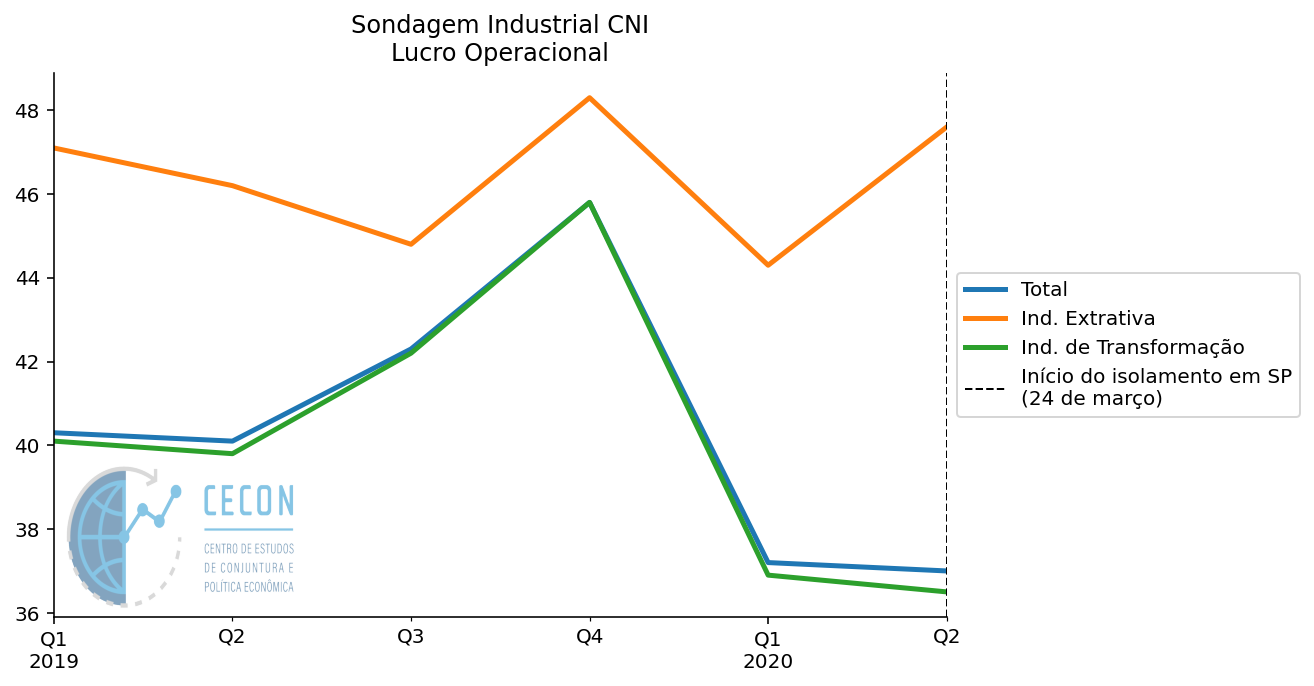
\includegraphics[width=.9\linewidth]{obipy-resources/62e383af79e91b63c7fc98dd7fb55b3c3ececcb9/82d95fa798d4ba22575a10087adf5c823956433e.png}
\end{center}

\item Situação Financeira
\label{sec:org3c36a53}

\begin{verbatim}
<Figure size 576x360 with 2 Axes>
\end{verbatim}


\begin{center}
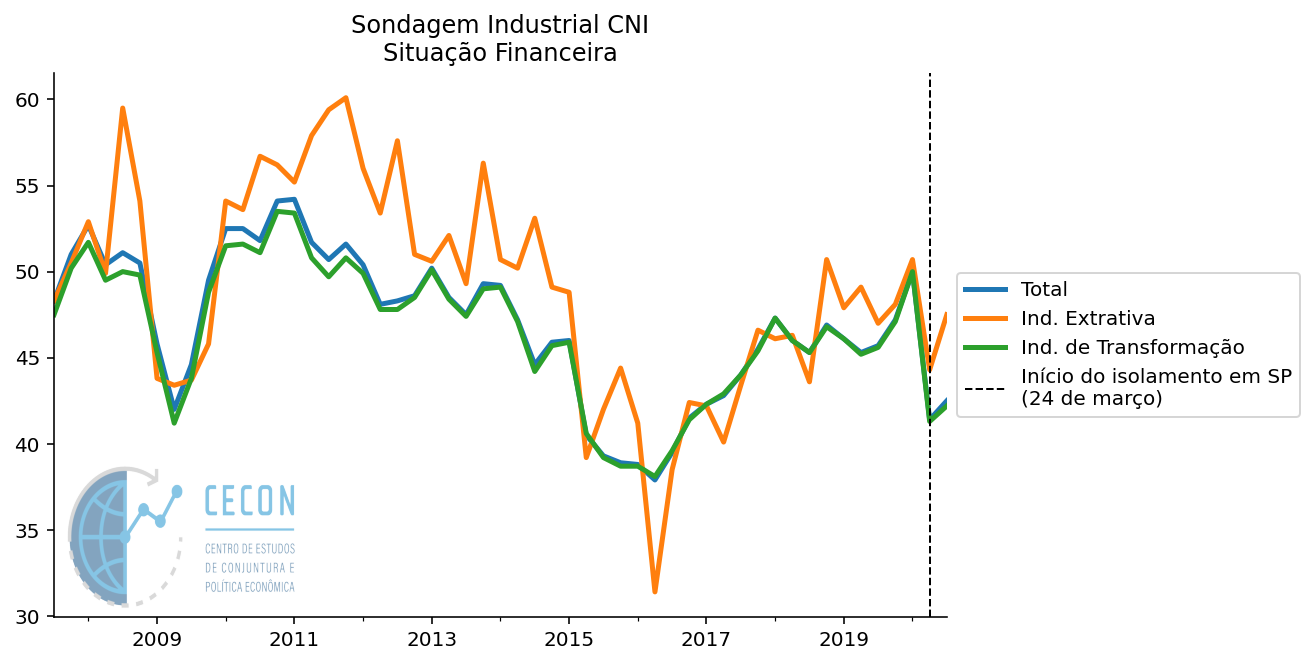
\includegraphics[width=.9\linewidth]{obipy-resources/62e383af79e91b63c7fc98dd7fb55b3c3ececcb9/bf403eed7affd3cdac032cea98157acdb3c29b05.png}
\end{center}


\item Acesso a Crédito
\label{sec:org78070ab}

\begin{verbatim}
<Figure size 576x360 with 2 Axes>
\end{verbatim}


\begin{center}
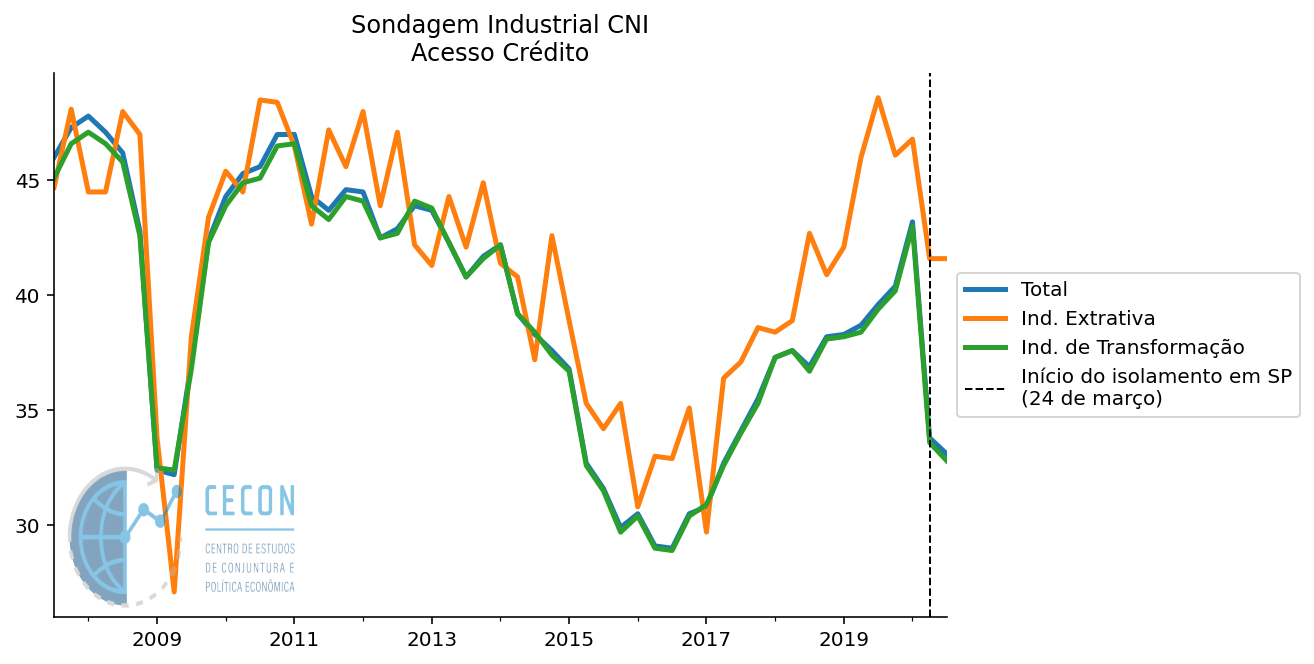
\includegraphics[width=.9\linewidth]{obipy-resources/62e383af79e91b63c7fc98dd7fb55b3c3ececcb9/d8b87eca93910a125a0efab8c3c2d1ff4bc1d07b.png}
\end{center}
\end{enumerate}

\subsection{Indicadores de antecedente}
\label{sec:org6d20eb3}

\subsubsection{Composite Leading index (\href{https://stats.oecd.org/Index.aspx?DataSetCode=MEI\_CLI}{CLI})}
\label{sec:org32696df}

WARNING:root:OECD + Major Six NME not found in regex
WARNING:root:Major Five Asia not found in regex
WARNING:root:Four Big European not found in regex
WARNING:root:G7 not found in ISO2
WARNING:root:NAFTA not found in regex
WARNING:root:OECD - Total not found in regex
WARNING:root:OECD - Europe not found in regex
WARNING:root:Euro area (19 countries) not found in regex
WARNING:root:OECD total  not found in regex

\begin{verbatim}
<Figure size 576x360 with 1 Axes>
\end{verbatim}


\begin{center}
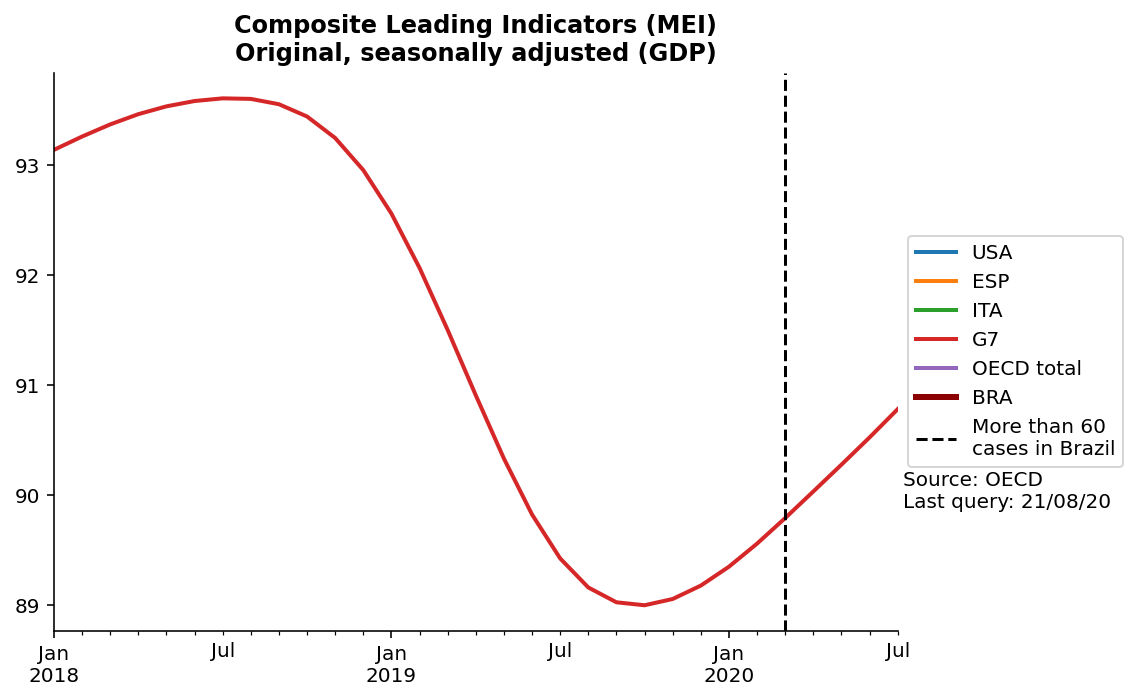
\includegraphics[width=.9\linewidth]{obipy-resources/62e383af79e91b63c7fc98dd7fb55b3c3ececcb9/9bcf6d9f78953ccf19a8f910062819f29e1f69ea.png}
\end{center}


\subsubsection{Consumer Confidence index (\href{https://stats.oecd.org/Index.aspx?DataSetCode=MEI\_CCI}{CCI})}
\label{sec:orgf957ce0}

\emph{home/gpetrini}.local/lib/python3.8/site-packages/pandas/core/indexing.py:1762: PerformanceWarning: indexing past lexsort depth may impact performance.
  return self.\_getitem\_tuple(key)
WARNING:root:OECD + Major Six NME not found in regex
WARNING:root:Major Five Asia not found in regex
WARNING:root:Four Big European not found in regex
WARNING:root:G7 not found in ISO2
WARNING:root:NAFTA not found in regex
WARNING:root:OECD - Total not found in regex
WARNING:root:OECD - Europe not found in regex
WARNING:root:Euro area (19 countries) not found in regex
WARNING:root:OECD total  not found in regex

\begin{verbatim}
<Figure size 576x360 with 1 Axes>
\end{verbatim}


\begin{center}
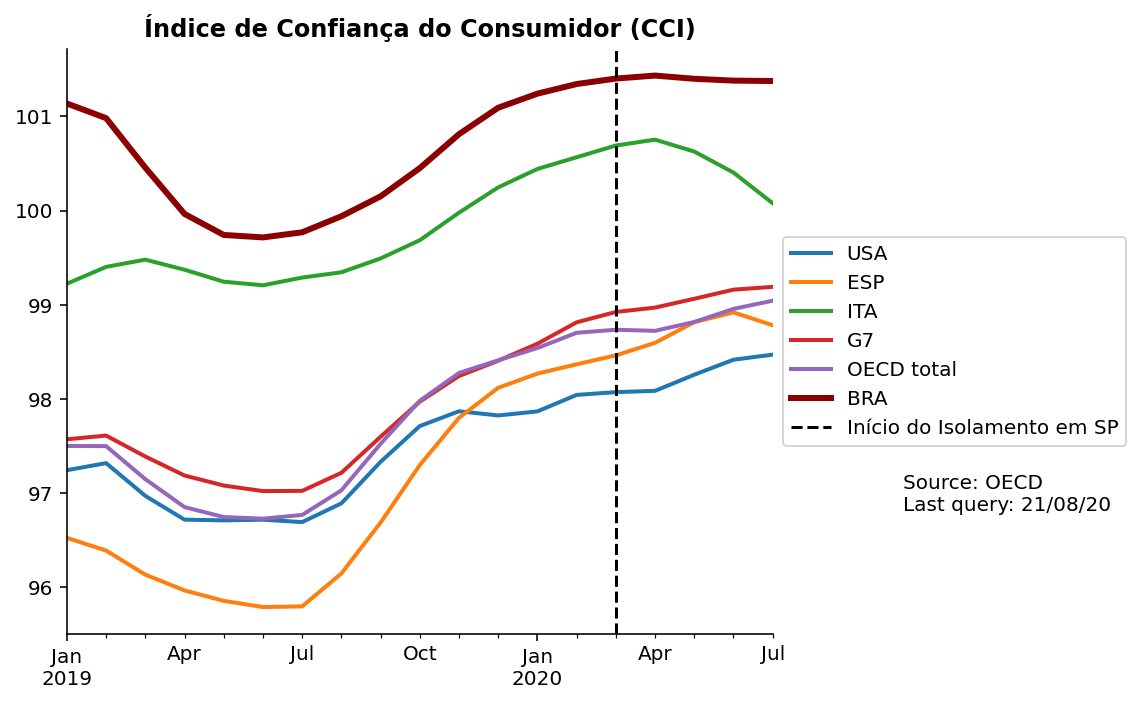
\includegraphics[width=.9\linewidth]{obipy-resources/62e383af79e91b63c7fc98dd7fb55b3c3ececcb9/f68f8b6cb09da9311b88232927b50a8f0f94cb40.png}
\end{center}

\subsection{Risco}
\label{sec:orgf957c73}

\subsubsection{EMBI+ (JP Morgan)}
\label{sec:orgd660997}

\begin{verbatim}
<Figure size 576x360 with 2 Axes>
\end{verbatim}


\begin{center}
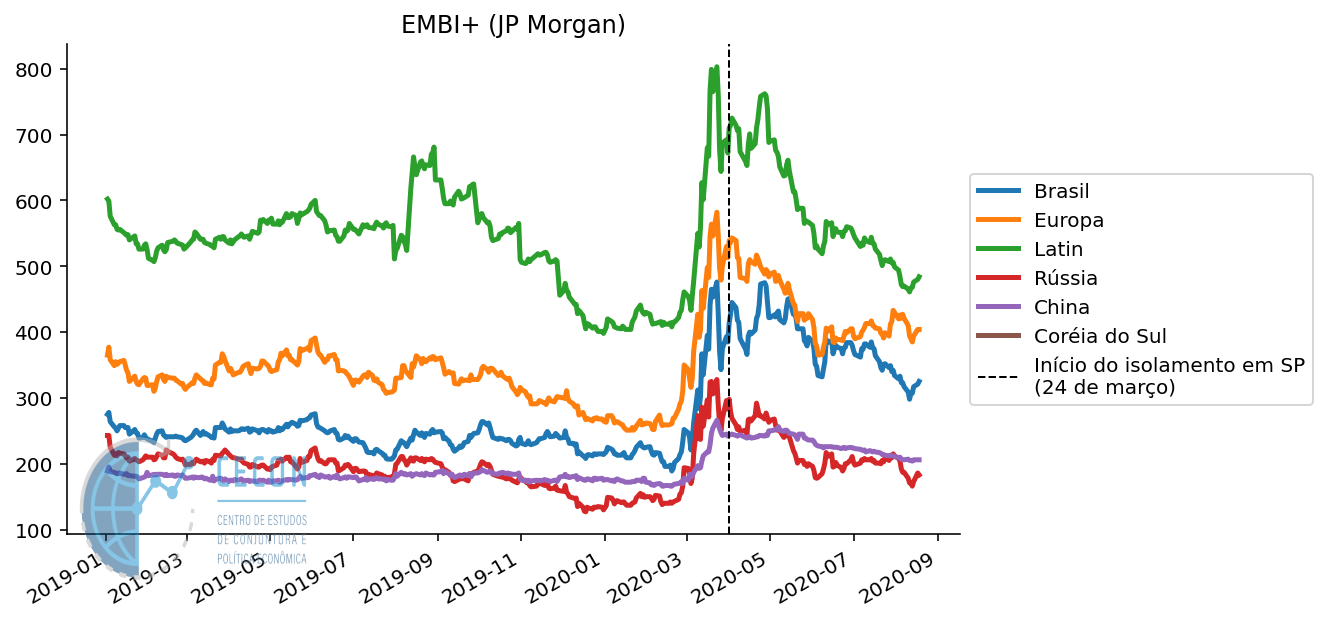
\includegraphics[width=.9\linewidth]{obipy-resources/62e383af79e91b63c7fc98dd7fb55b3c3ececcb9/c50dfc43d174b7c73e73e951c62430709a829874.png}
\end{center}


\subsection{Incerteza}
\label{sec:org8cd0d27}



\subsubsection{Indicador de Incerteza (IIE-Br)}
\label{sec:org261cc29}

\begin{verbatim}
<Figure size 2400x1500 with 2 Axes>
\end{verbatim}


\begin{center}
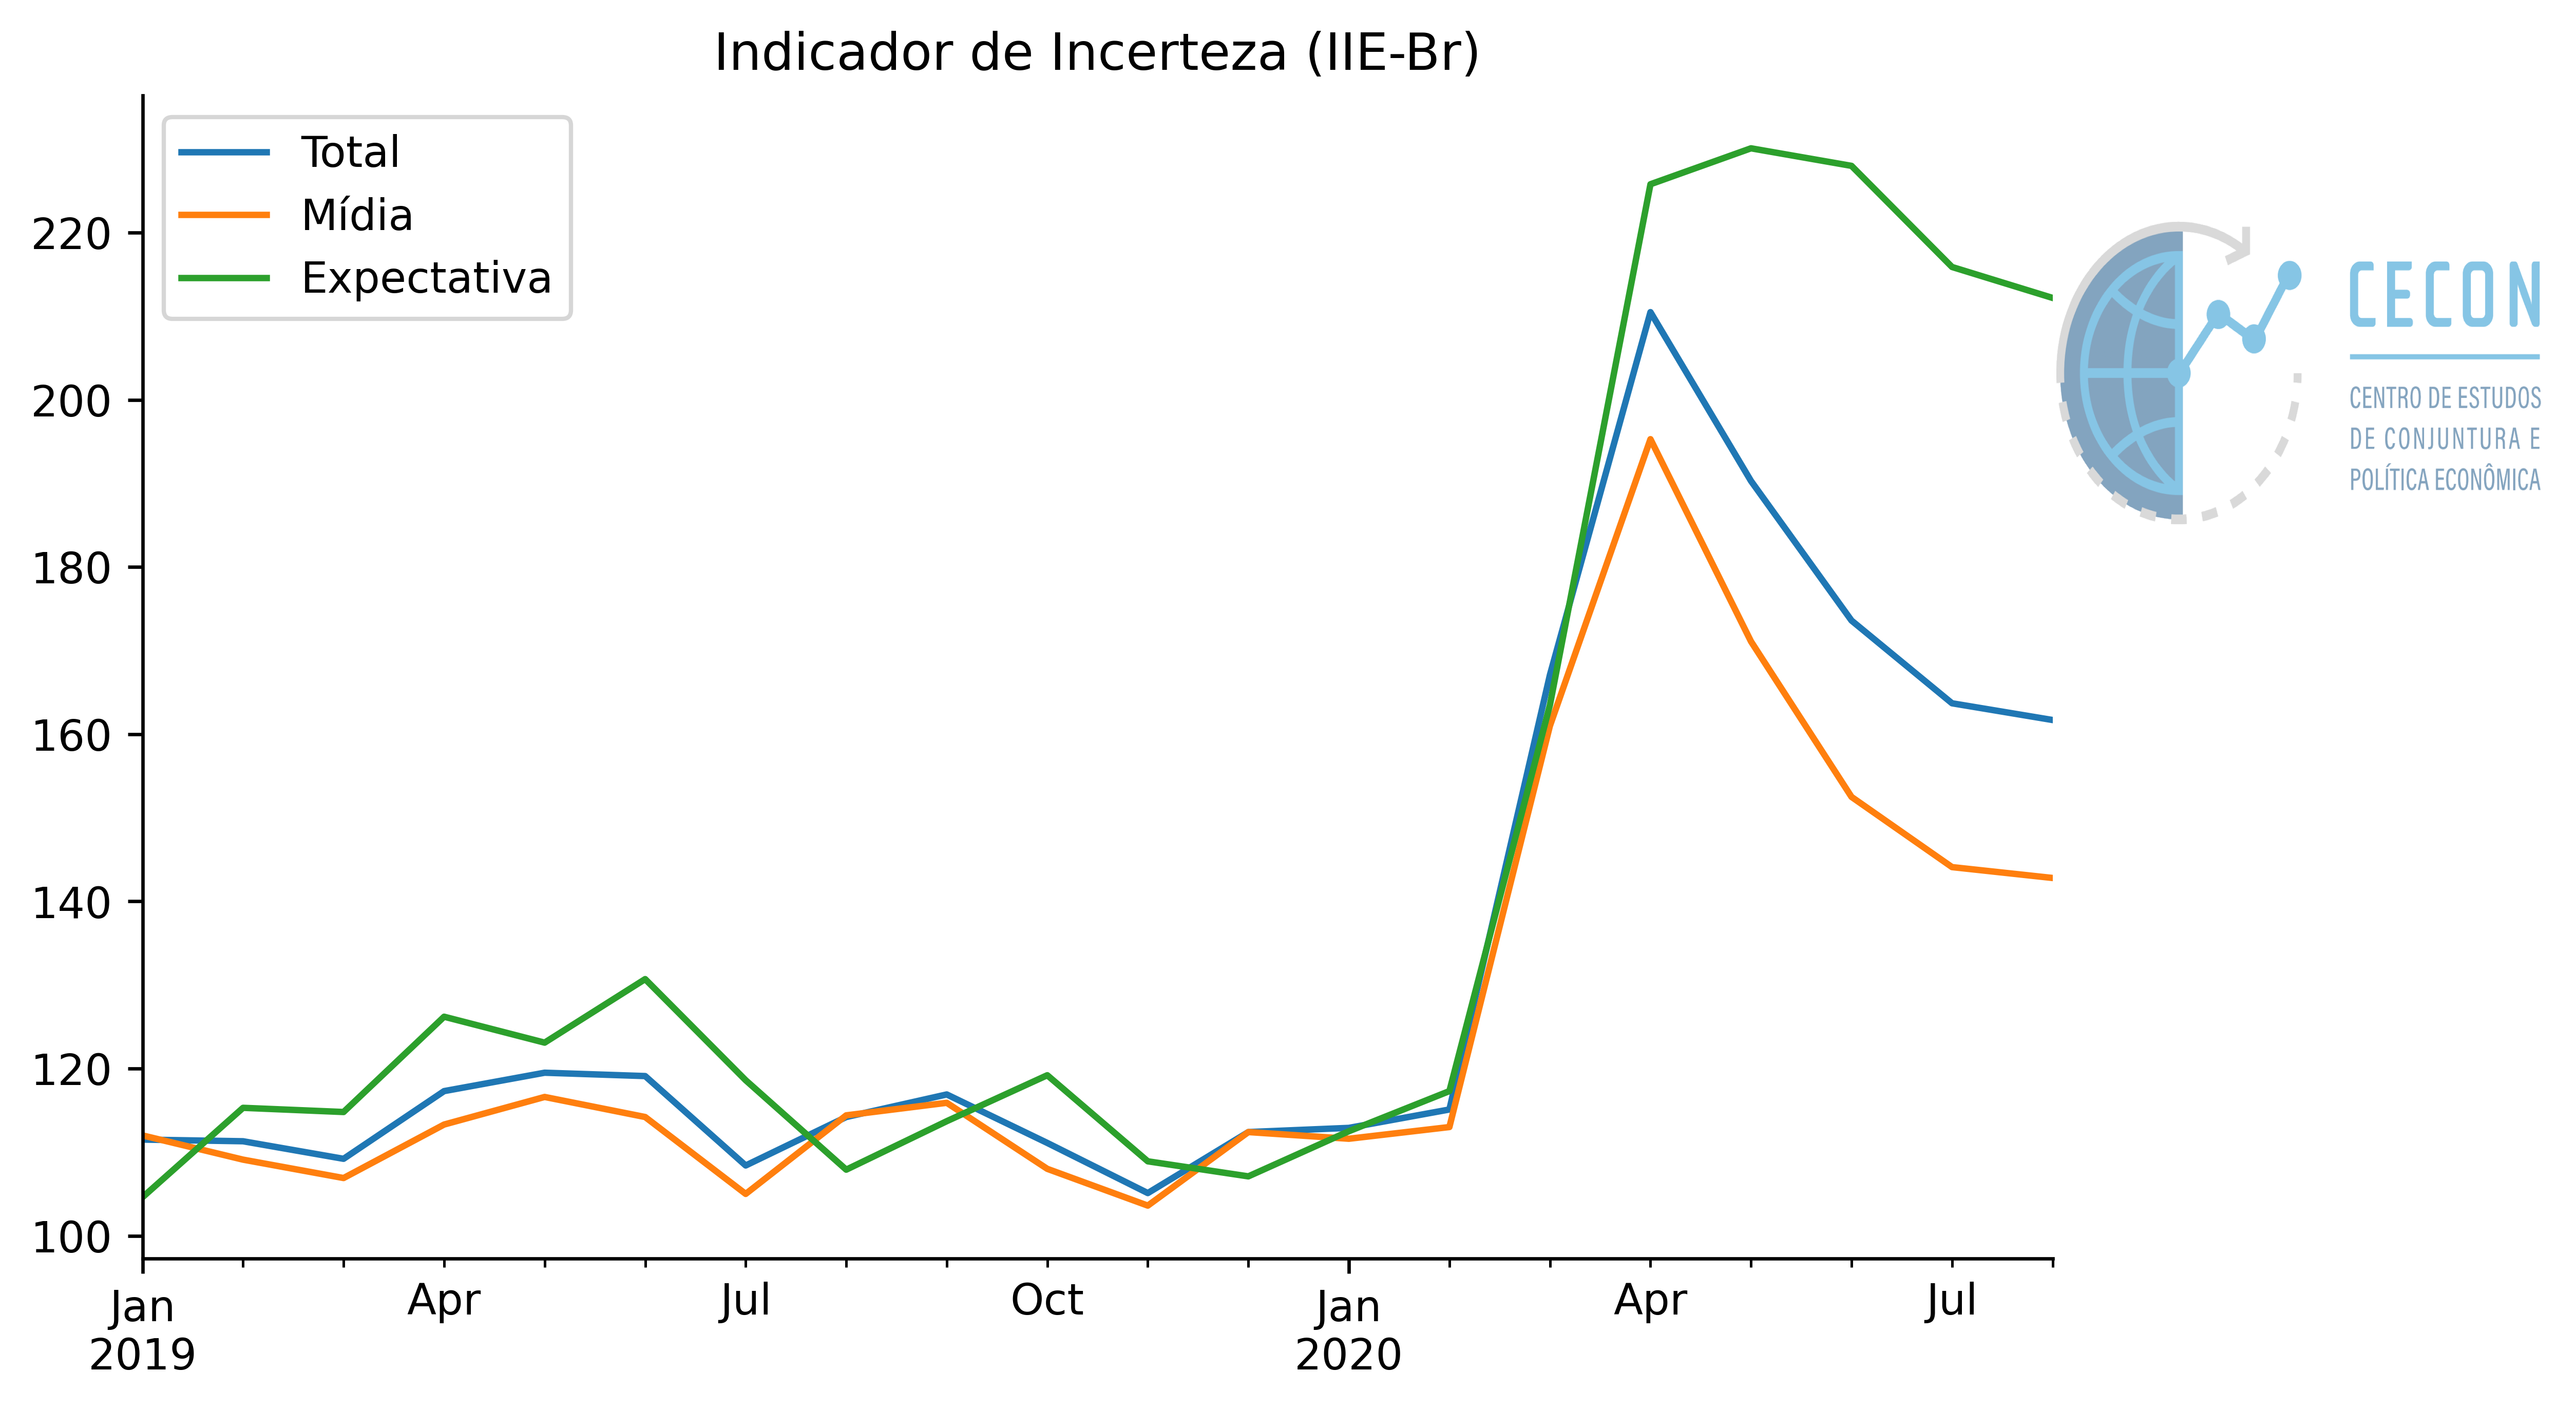
\includegraphics[width=.9\linewidth]{obipy-resources/62e383af79e91b63c7fc98dd7fb55b3c3ececcb9/c5efa72595cc12bf613b1062622f61c3df58ecab.png}
\end{center}


\subsubsection{Indicador de Confiança Empresarial}
\label{sec:org49b67af}

\begin{verbatim}
<Figure size 2400x1500 with 2 Axes>
\end{verbatim}


\begin{center}
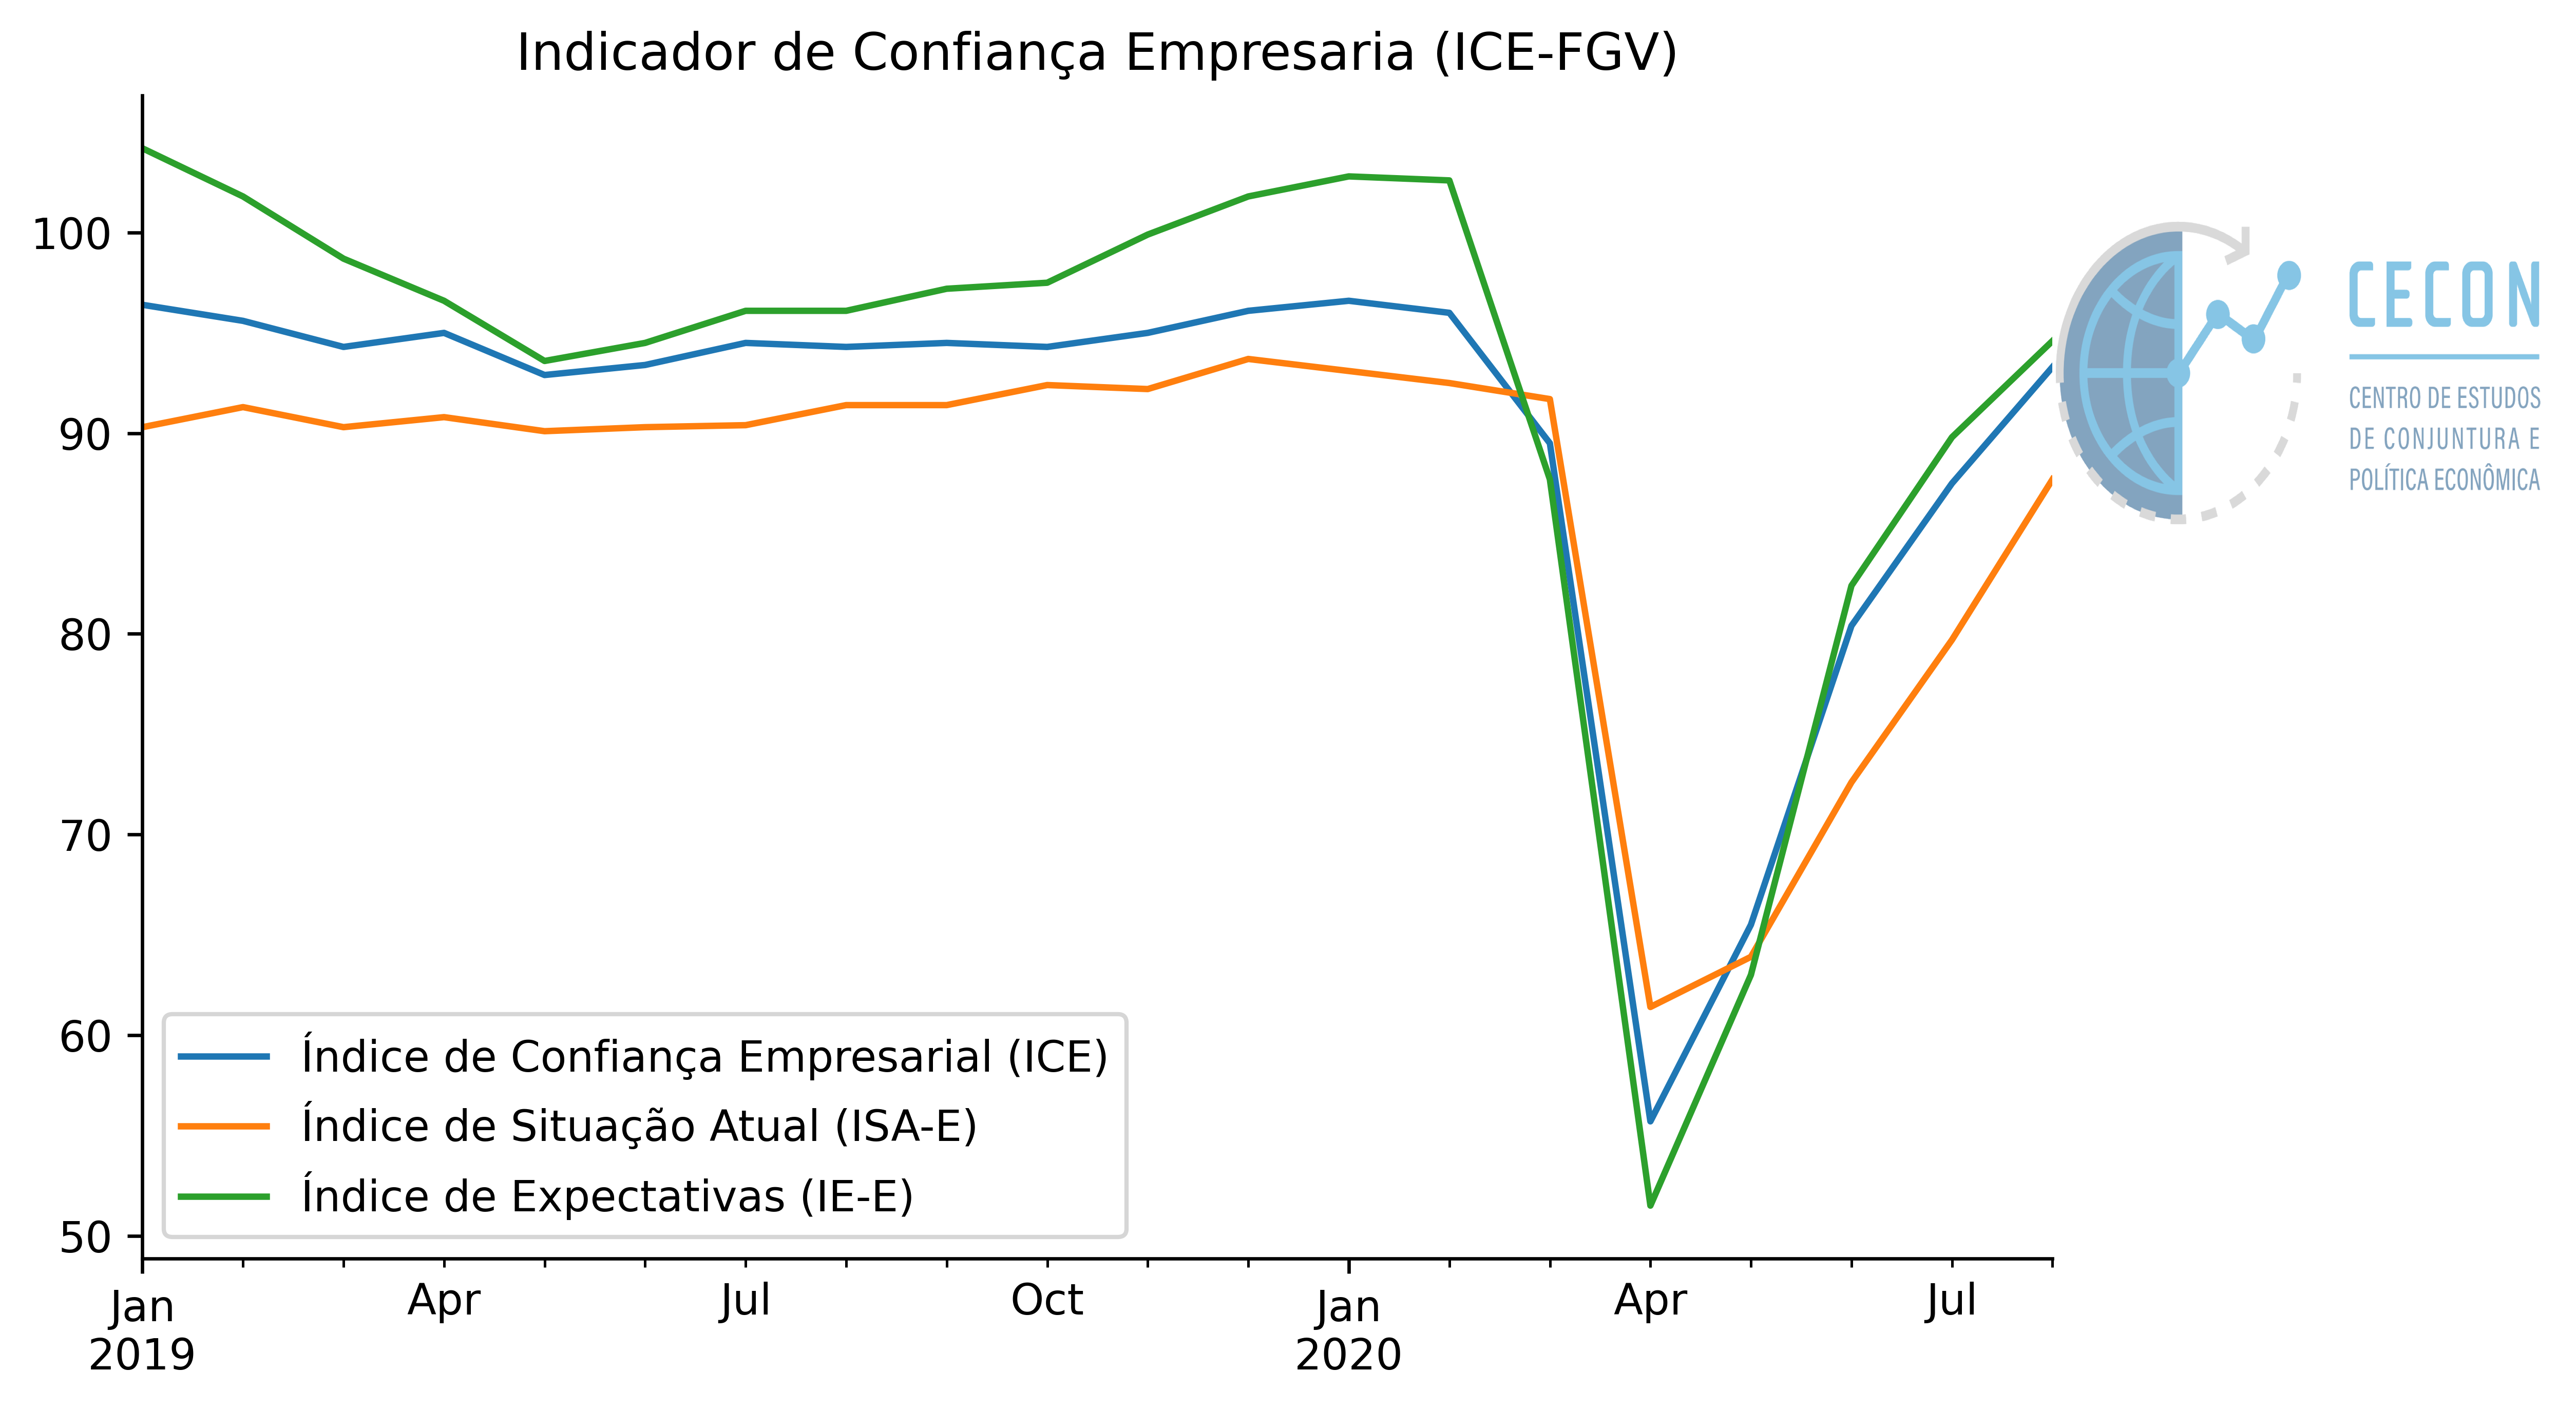
\includegraphics[width=.9\linewidth]{obipy-resources/62e383af79e91b63c7fc98dd7fb55b3c3ececcb9/8e38298178125842685b068036bdce559fd6ab01.png}
\end{center}

\section{Atividade}
\label{sec:orgf04114a}

\subsection{Crédito}
\label{sec:orgf7c3d51}


\subsubsection{Saldo}
\label{sec:org495ee79}

\begin{enumerate}
\item Pessoa jurídica
\label{sec:orgd30092b}

\begin{verbatim}
<Figure size 576x360 with 2 Axes>
\end{verbatim}


\begin{center}
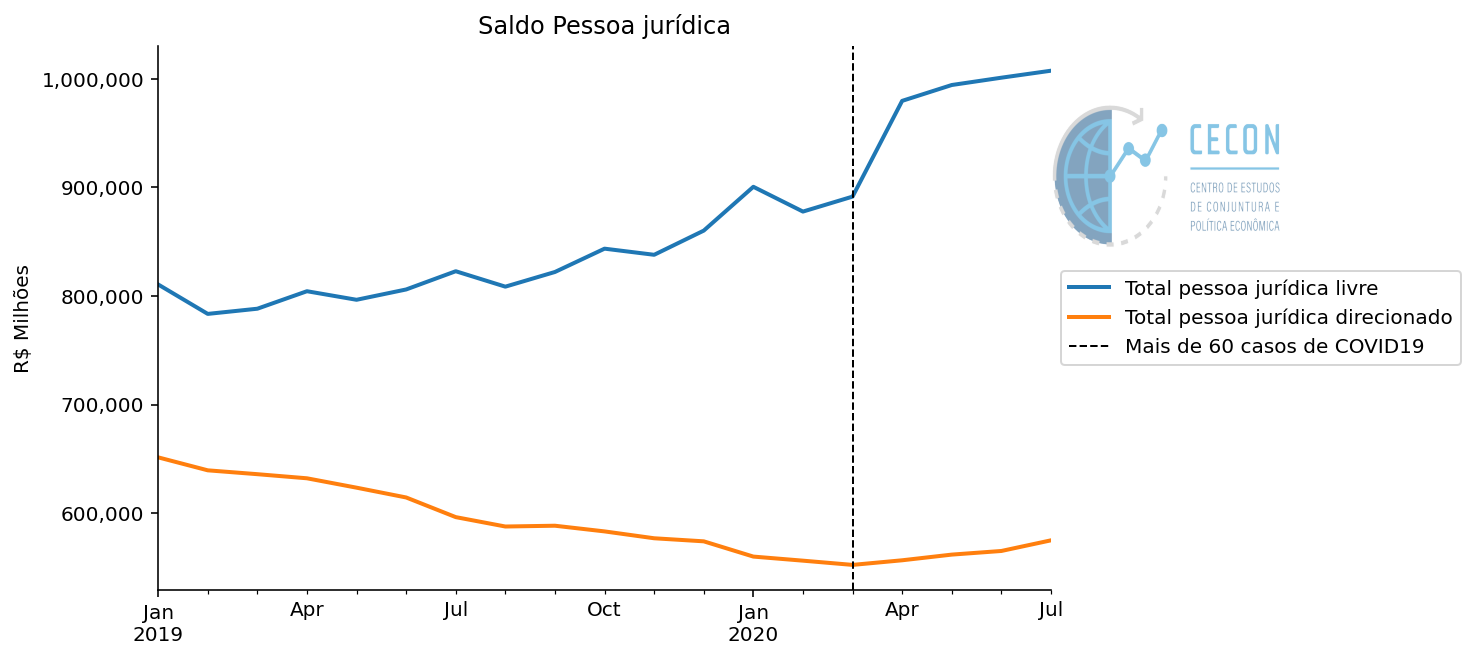
\includegraphics[width=.9\linewidth]{obipy-resources/62e383af79e91b63c7fc98dd7fb55b3c3ececcb9/402de444762880e51b3a602c504b7e8d63732349.png}
\end{center}


\begin{verbatim}
<Figure size 576x360 with 2 Axes>
\end{verbatim}


\begin{center}
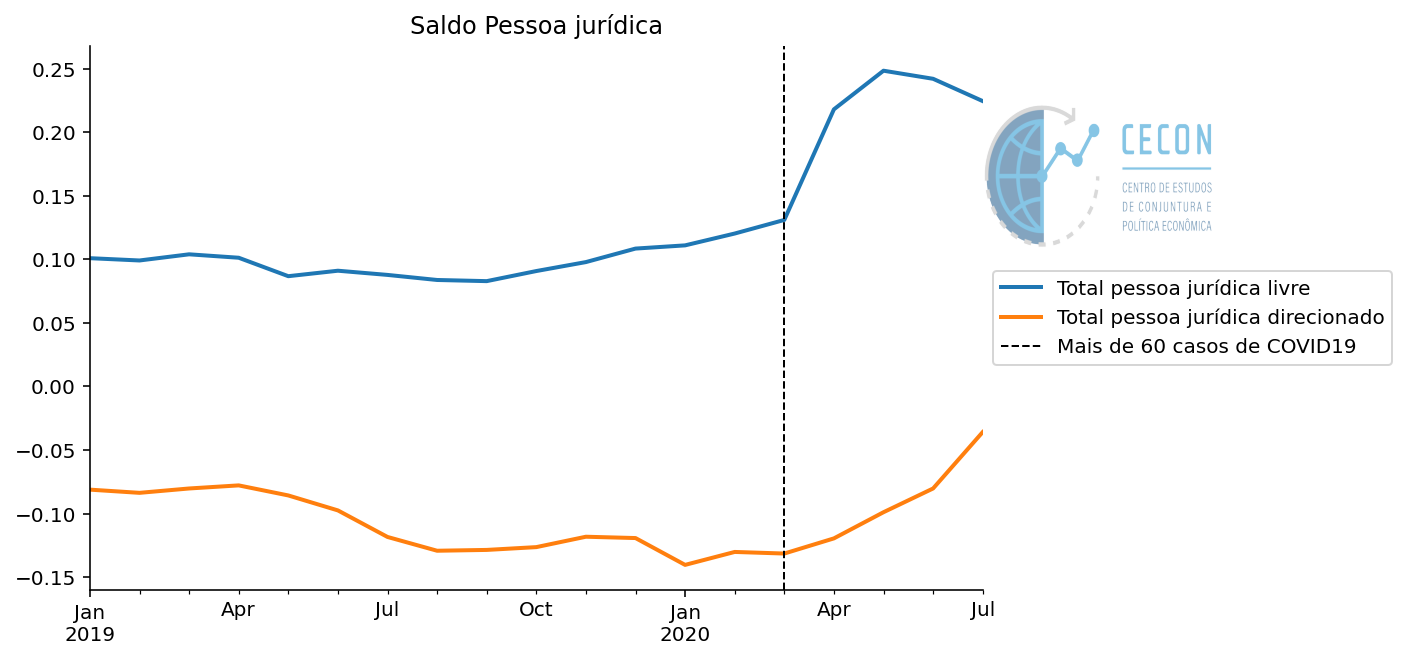
\includegraphics[width=.9\linewidth]{obipy-resources/62e383af79e91b63c7fc98dd7fb55b3c3ececcb9/8ade2681015bf89863078900a6d91c53bd592f3b.png}
\end{center}

\item Pessoa física
\label{sec:orgf30bca5}

\begin{verbatim}
<Figure size 576x360 with 2 Axes>
\end{verbatim}


\begin{center}
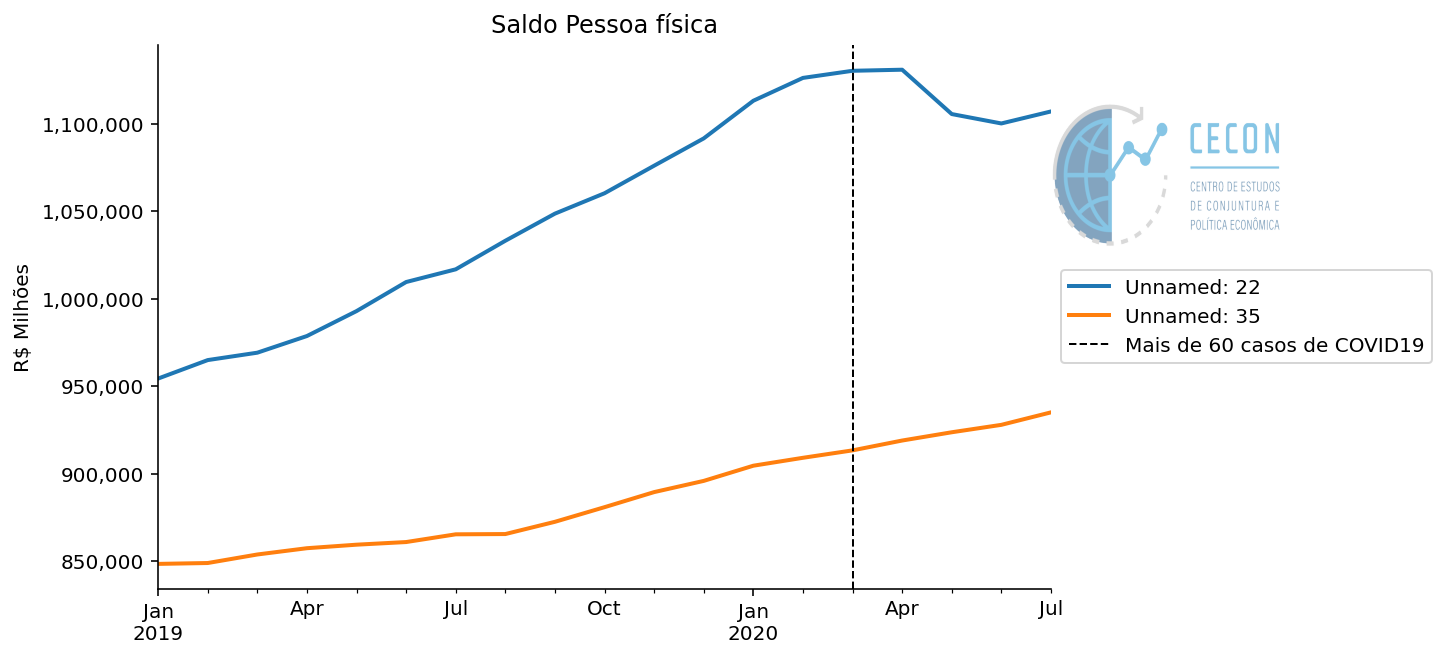
\includegraphics[width=.9\linewidth]{obipy-resources/62e383af79e91b63c7fc98dd7fb55b3c3ececcb9/c5ebb89c192628d7cec923eb13d6356df012028a.png}
\end{center}

\begin{verbatim}
<Figure size 576x360 with 2 Axes>
\end{verbatim}


\begin{center}
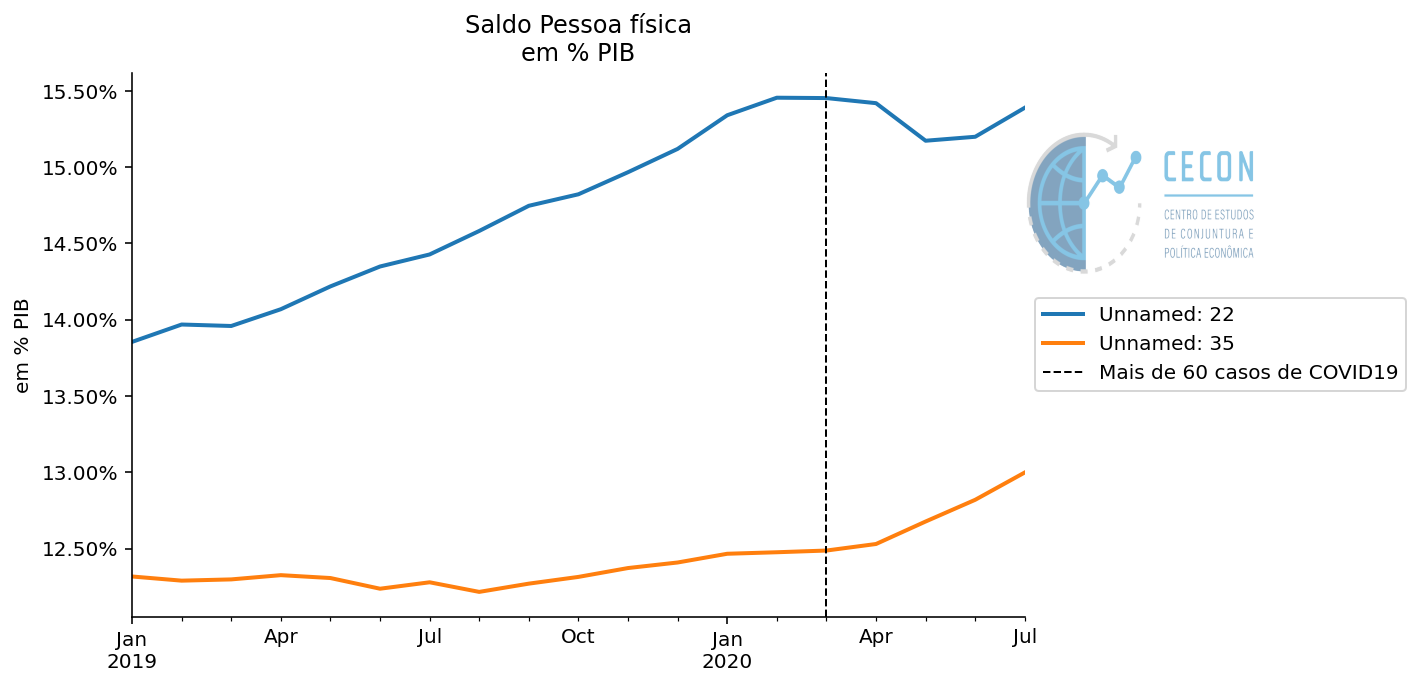
\includegraphics[width=.9\linewidth]{obipy-resources/62e383af79e91b63c7fc98dd7fb55b3c3ececcb9/b694dfa6b6aa8de15c823bc95e21ec965d607fee.png}
\end{center}

\item Crédito ampliado
\label{sec:org3ae77ba}

\begin{verbatim}
<Figure size 576x360 with 2 Axes>
\end{verbatim}


\begin{center}
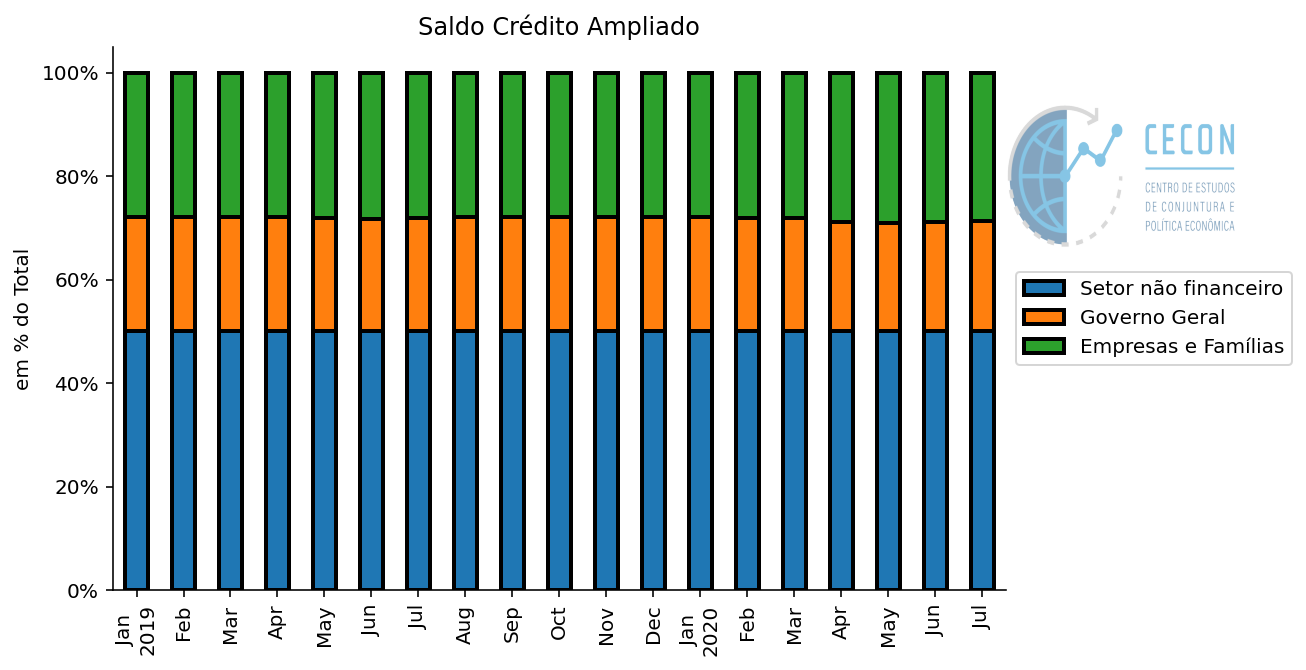
\includegraphics[width=.9\linewidth]{obipy-resources/62e383af79e91b63c7fc98dd7fb55b3c3ececcb9/fc25f4901d8007b52b37c8cc10e4620bc37873f2.png}
\end{center}

\begin{verbatim}
<Figure size 576x360 with 2 Axes>
\end{verbatim}


\begin{center}
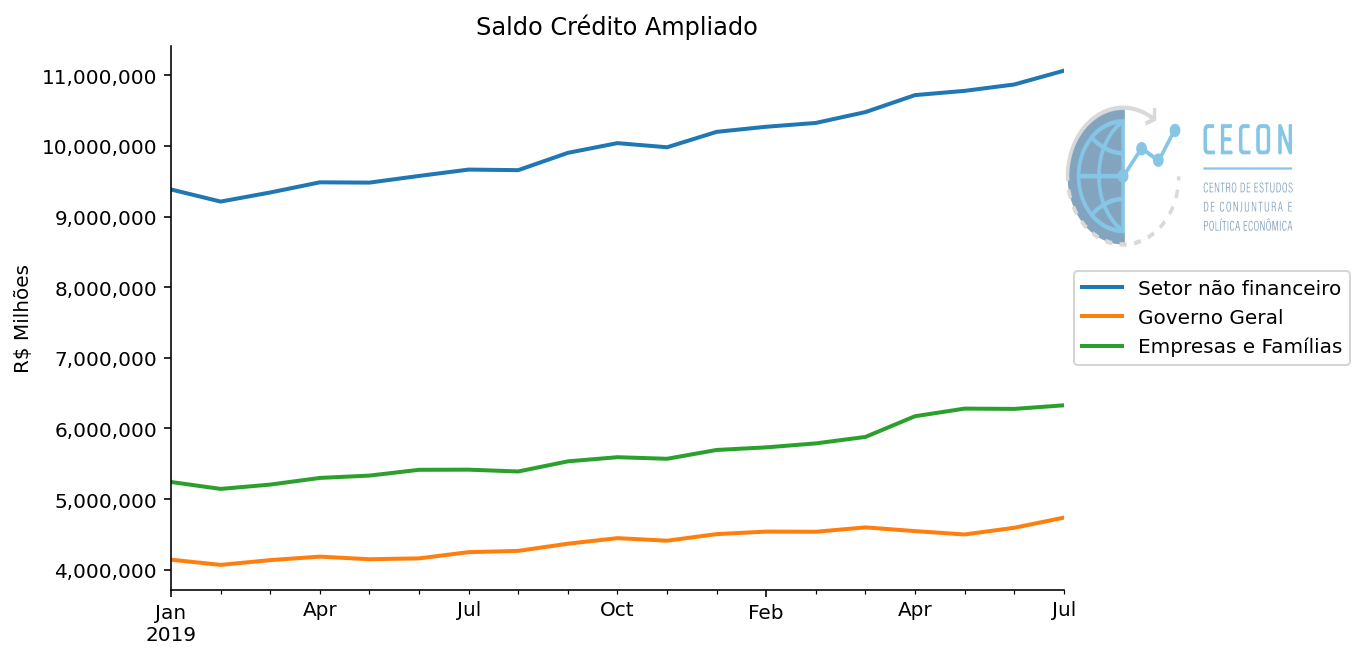
\includegraphics[width=.9\linewidth]{obipy-resources/62e383af79e91b63c7fc98dd7fb55b3c3ececcb9/285a93936f0519f57c3f51e4597e9bc013c3ab1a.png}
\end{center}


\begin{verbatim}
<Figure size 576x360 with 2 Axes>
\end{verbatim}


\begin{center}
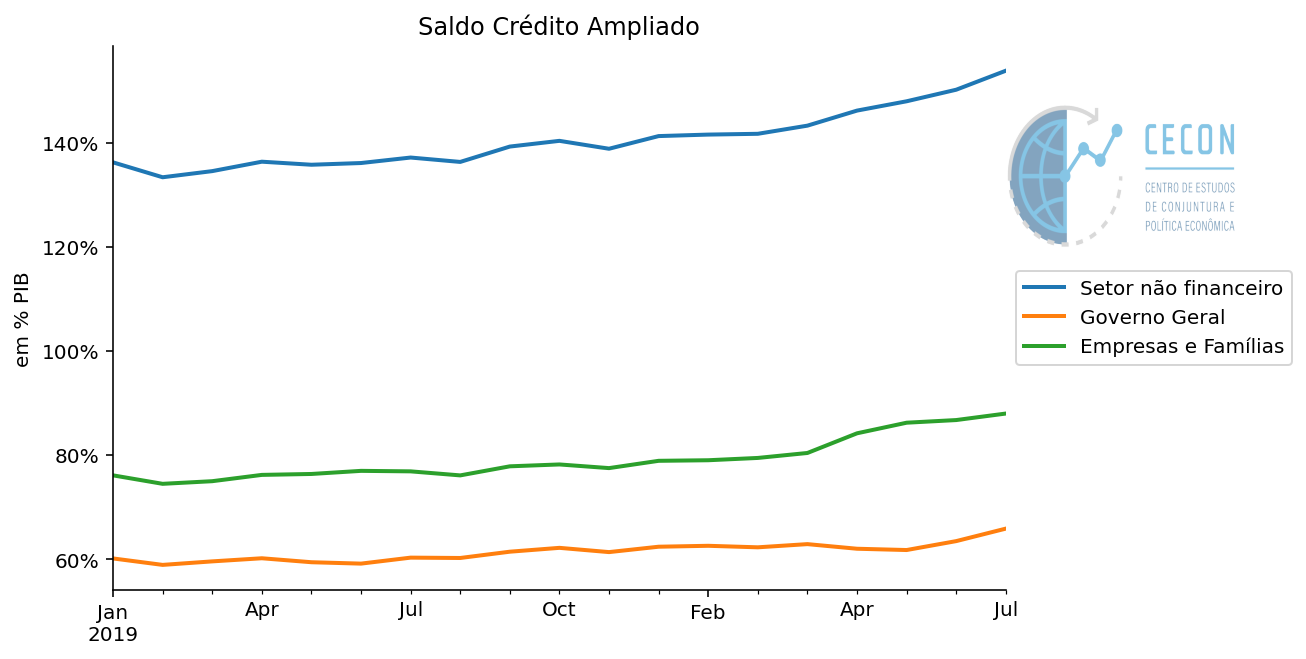
\includegraphics[width=.9\linewidth]{obipy-resources/62e383af79e91b63c7fc98dd7fb55b3c3ececcb9/71e2f6f170d1eae4c7e08b6bb69381e2fc6bfa43.png}
\end{center}

\item Crédito direcionado
\label{sec:org60530d1}


\begin{verbatim}
<Figure size 576x360 with 2 Axes>
\end{verbatim}


\begin{center}
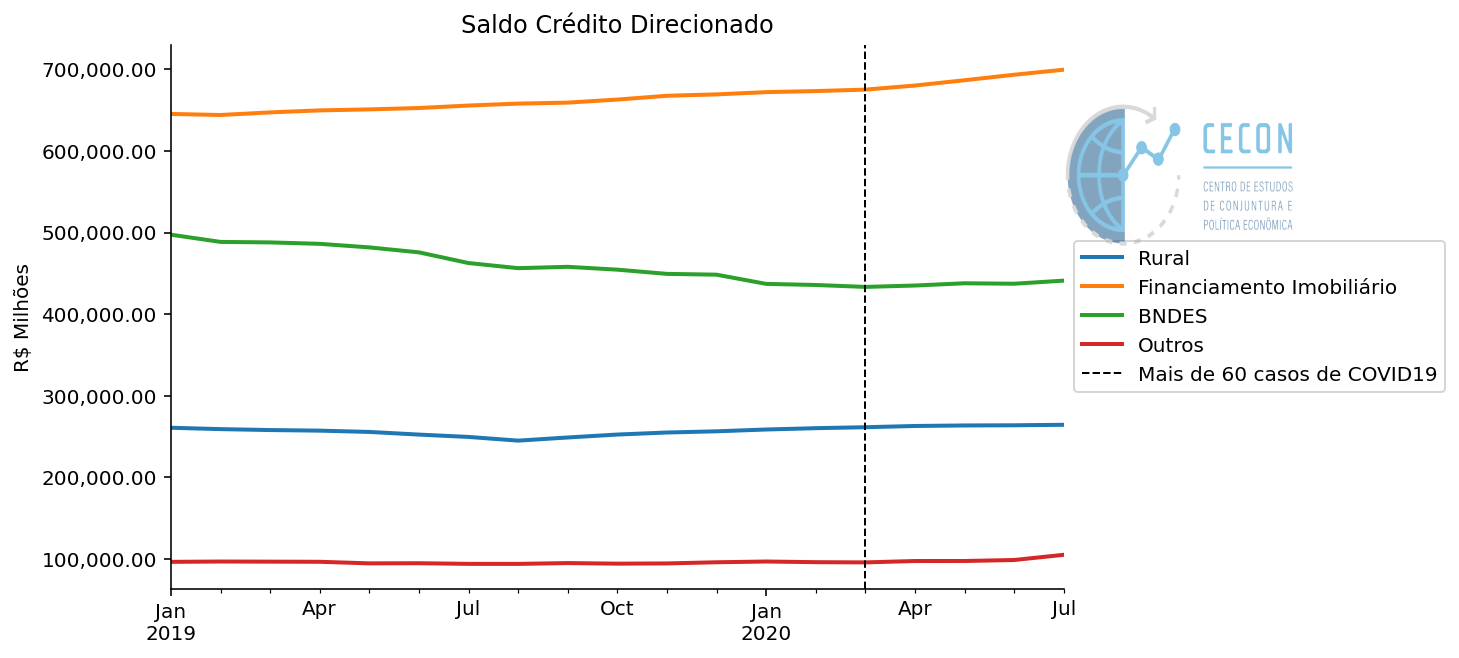
\includegraphics[width=.9\linewidth]{obipy-resources/62e383af79e91b63c7fc98dd7fb55b3c3ececcb9/8e80f62dee7a7da5353be6056c7d954dc453835e.png}
\end{center}

\begin{verbatim}
<Figure size 576x360 with 2 Axes>
\end{verbatim}


\begin{center}
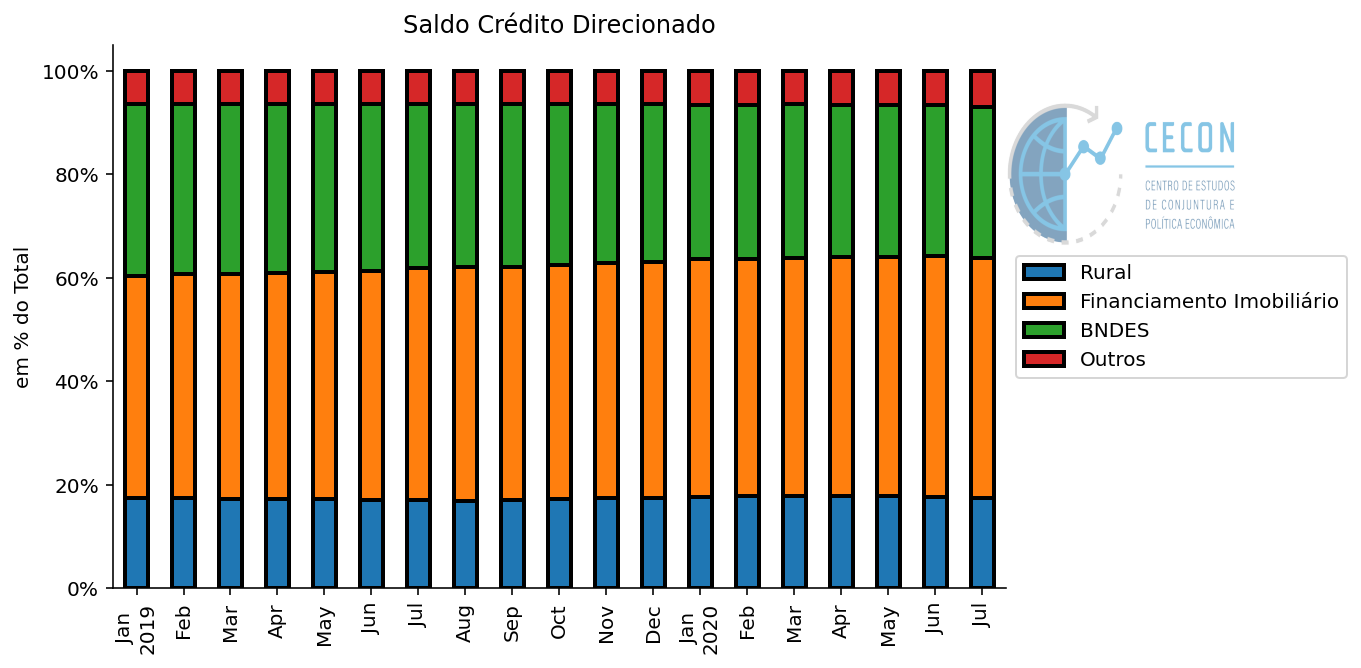
\includegraphics[width=.9\linewidth]{obipy-resources/62e383af79e91b63c7fc98dd7fb55b3c3ececcb9/9a2b55ba48387fe773ae71f452b084dae90c5a91.png}
\end{center}

\begin{verbatim}
<Figure size 576x360 with 2 Axes>
\end{verbatim}


\begin{center}
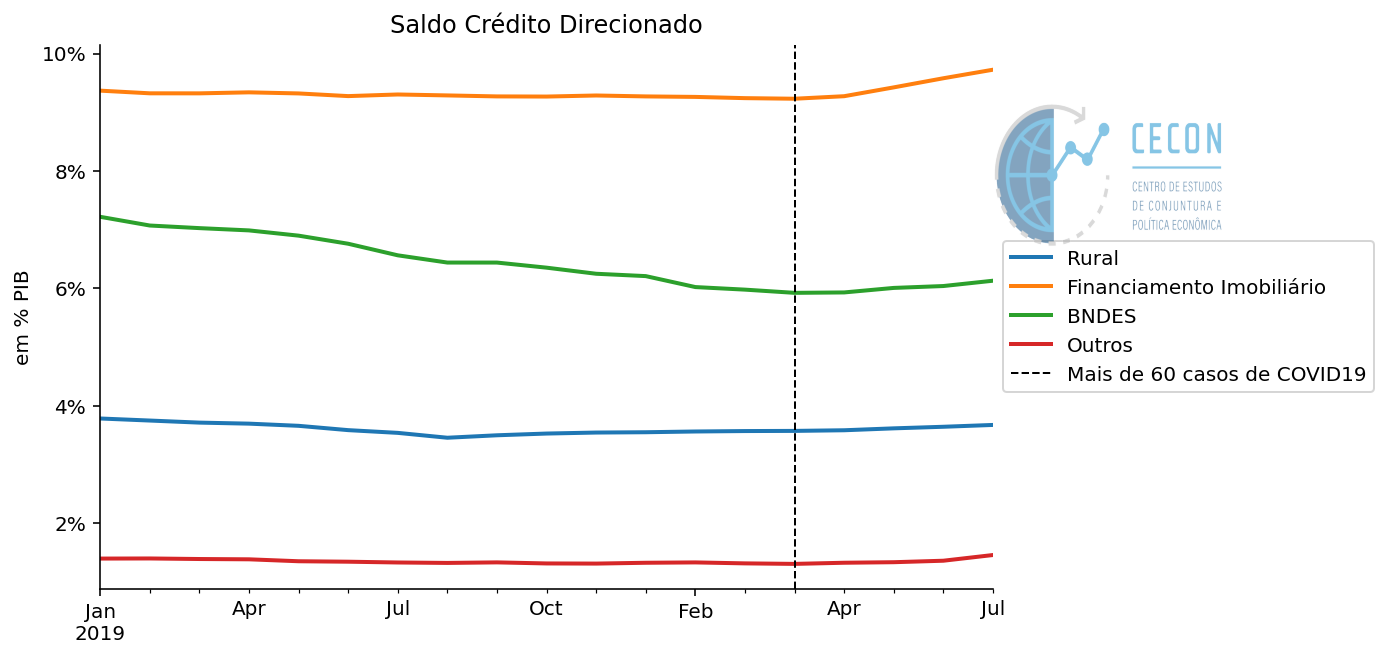
\includegraphics[width=.9\linewidth]{obipy-resources/62e383af79e91b63c7fc98dd7fb55b3c3ececcb9/9d5911f91378331c30c8ae9b513d4af5c47cd126.png}
\end{center}
\end{enumerate}



\subsection{IBCBr}
\label{sec:org72b8991}

\begin{verbatim}
<Figure size 576x360 with 2 Axes>
\end{verbatim}


\begin{center}
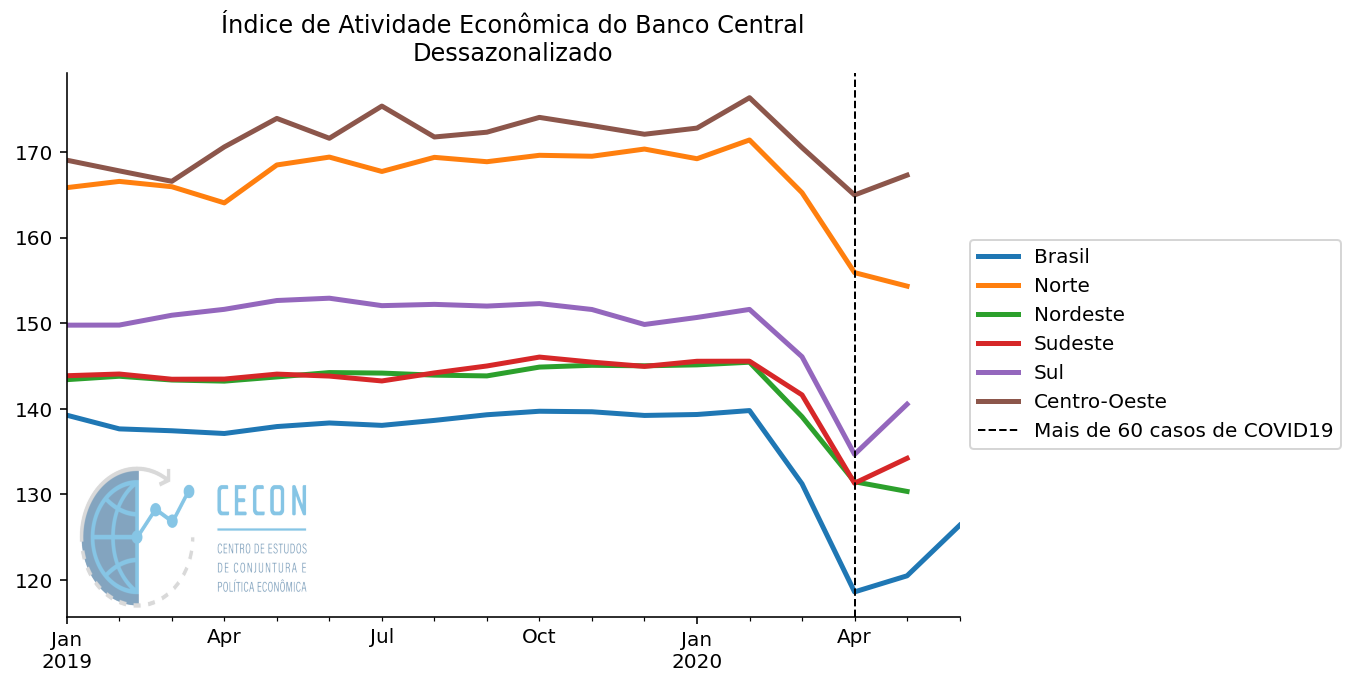
\includegraphics[width=.9\linewidth]{obipy-resources/62e383af79e91b63c7fc98dd7fb55b3c3ececcb9/867e8a85521aa7667c388ddb9c5027a1ada952bb.png}
\end{center}

\subsection{PIB (Contas Nacionais)}
\label{sec:org4af1a2d}

Archive:  Tab\_Compl\_CNT.zip
  inflating: Tab\_Compl\_CNT\_1T20.xls  

\subsubsection{Trimestre Contra trimestre imediatamente anterior}
\label{sec:org9bdbe0c}

2019Q2    0.005406
2019Q3    0.004618
2019Q4    0.003655
2020Q1   -0.015394
Freq: Q-DEC, Name: PIB, dtype: float64

\begin{verbatim}
<Figure size 648x288 with 2 Axes>
\end{verbatim}


\begin{center}
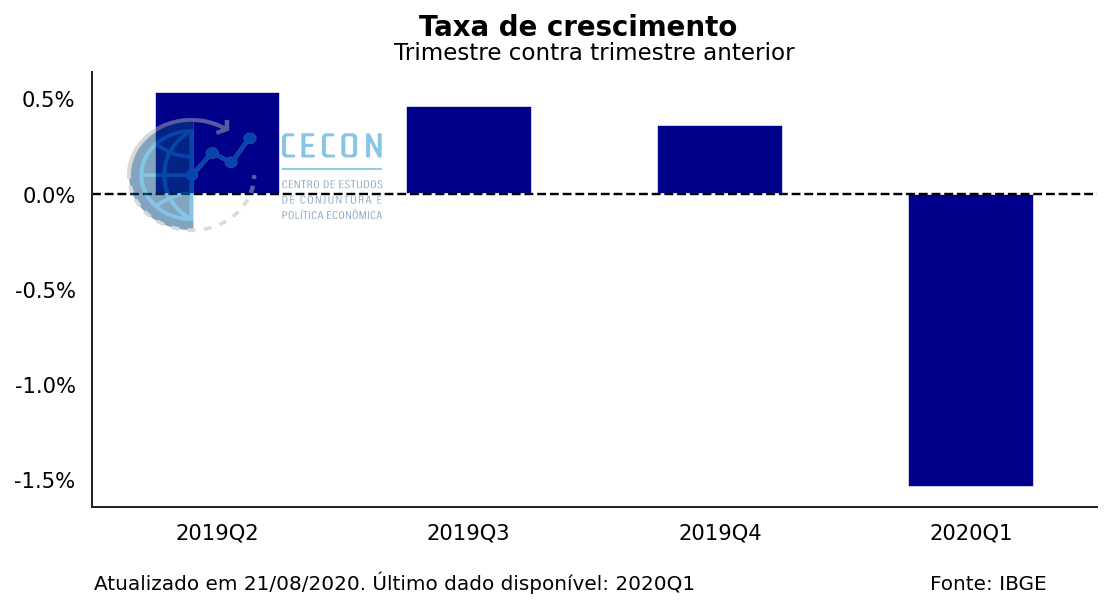
\includegraphics[width=.9\linewidth]{obipy-resources/62e383af79e91b63c7fc98dd7fb55b3c3ececcb9/ae1515a7b487b55149c37fa44d319f5deb1387b7.png}
\end{center}

\begin{enumerate}
\item Agropecuária
\label{sec:org18364df}

\begin{verbatim}
<Figure size 648x288 with 2 Axes>
\end{verbatim}


\begin{center}
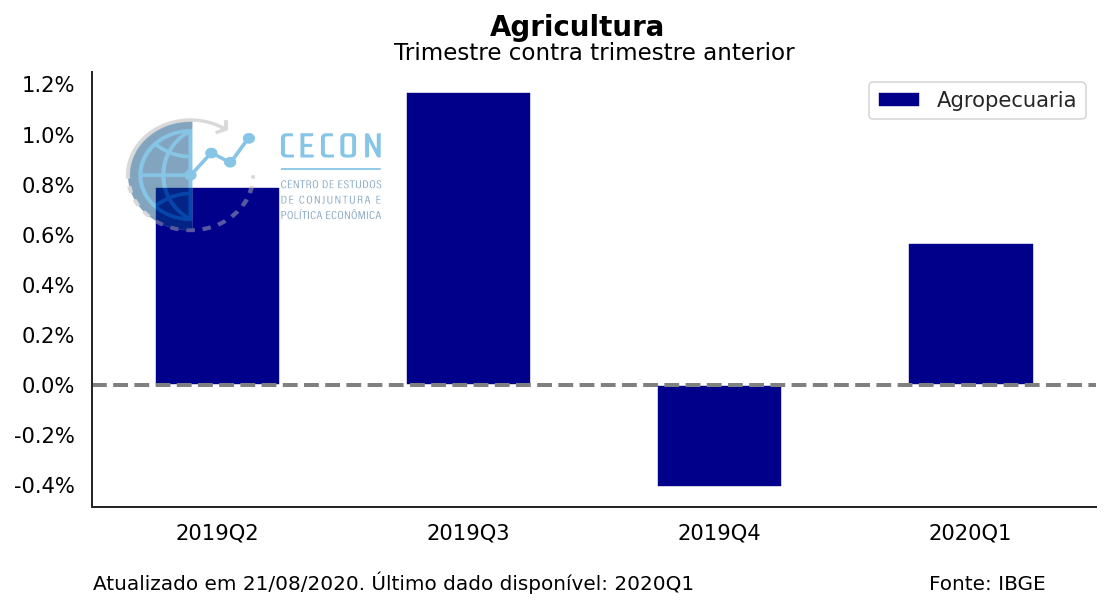
\includegraphics[width=.9\linewidth]{obipy-resources/62e383af79e91b63c7fc98dd7fb55b3c3ececcb9/3567d5d74a87a0022c1b5d021b8202e9643e9c6d.png}
\end{center}

\item Indústria
\label{sec:org657ab48}

\begin{verbatim}
        Industria Extrativa  Industria de Transformacao  Eletricidade e agua  \
2019Q2            -0.030796                    0.015653            -0.004612   
2019Q3             0.112907                   -0.008735            -0.013919   
2019Q4             0.006668                    0.001203             0.002735   
2020Q1            -0.032339                   -0.013738            -0.001341   

        Construcao  Total Industria  
2019Q2    0.019130         0.006188  
2019Q3    0.008864         0.007511  
2019Q4   -0.023357         0.000195  
2020Q1   -0.023948        -0.013793  
\end{verbatim}


\url{file:///tmp/ob-ipython-html6Ut6v0.html}

\begin{verbatim}
<Figure size 648x288 with 2 Axes>
\end{verbatim}


\begin{center}
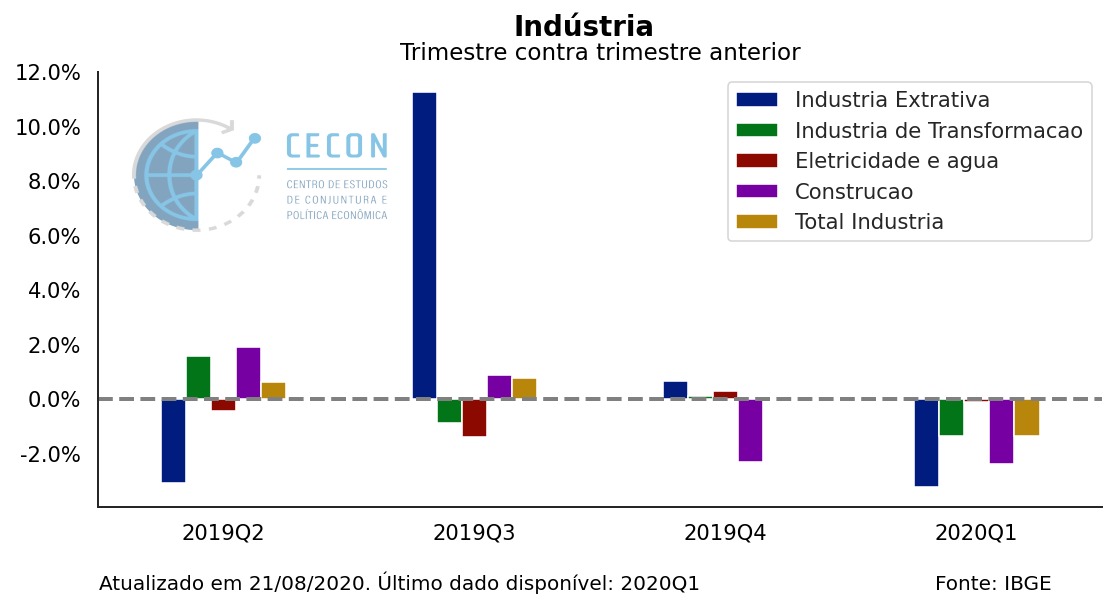
\includegraphics[width=.9\linewidth]{obipy-resources/62e383af79e91b63c7fc98dd7fb55b3c3ececcb9/bc5997d911634acc1c7a406cdbacc62dba75ab6a.png}
\end{center}


\item Serviços
\label{sec:org96390dc}

        Comercio  Transporte, armazenagem e correio  Informacao e comunicacao  $\backslash$
1996Q1       NaN                                NaN                       NaN   
1996Q2 -0.002371                          -0.028222                  0.015095   
1996Q3  0.025455                           0.036438                  0.021967   
1996Q4  0.015195                          -0.037310                 -0.001976   
1997Q1  0.002414                           0.040428                  0.011012   
\ldots{}          \ldots{}                                \ldots{}                       \ldots{}   
2019Q1  0.008961                          -0.002449                  0.011049   
2019Q2  0.006977                          -0.000455                  0.006743   
2019Q3  0.007517                          -0.003686                  0.010703   
2019Q4 -0.001857                           0.014547                  0.016215   
2020Q1 -0.007686                          -0.024192                 -0.019052   

        Atividades Financeiras  Atividades Imobiliarias  Outras atividades  $\backslash$
1996Q1                     NaN                      NaN                NaN   
1996Q2                0.001748                 0.006362          -0.005097   
1996Q3               -0.000033                 0.009057           0.002842   
1996Q4               -0.087280                -0.024478          -0.003531   
1997Q1                0.110854                 0.022929           0.014299   
\ldots{}                        \ldots{}                      \ldots{}                \ldots{}   
2019Q1                0.008045                 0.003100           0.001185   
2019Q2               -0.000677                 0.007525           0.003958   
2019Q3                0.013945                 0.002887           0.000598   
2019Q4                0.008249                 0.001962           0.008319   
2020Q1               -0.001175                 0.003511          -0.045997   

        ADM, defesa, etc  Total Servicos  
1996Q1               NaN             NaN  
1996Q2          0.008730        0.003606  
1996Q3          0.005202        0.016645  
1996Q4         -0.006725       -0.023475  
1997Q1         -0.000029        0.021750  
\ldots{}                  \ldots{}             \ldots{}  
2019Q1          0.004140        0.003870  
2019Q2         -0.002328        0.002439  
2019Q3         -0.007317        0.003180  
2019Q4          0.010108        0.006761  
2020Q1         -0.004807       -0.016362  

[97 rows x 8 columns]

\begin{verbatim}
<Figure size 648x288 with 2 Axes>
\end{verbatim}


\begin{center}
\includegraphics[width=.9\linewidth]{obipy-resources/62e383af79e91b63c7fc98dd7fb55b3c3ececcb9/16f20c74bddf18148bdc452e51837900c45e4ce3.png}
\end{center}

\item Demanda
\label{sec:org860d472}

        Consumo das Familias  Consumo do Governo      FBCF  Exportacao  $\backslash$
2019Q2              0.004122           -0.002895  0.024859   -0.023292   
2019Q3              0.004586           -0.003876  0.017226   -0.023973   
2019Q4              0.004198            0.004176 -0.026872    0.022656   
2020Q1             -0.019856            0.002393  0.030928   -0.009145   

        Importacao       PIB  
2019Q2    0.014682  0.005406  
2019Q3    0.024805  0.004618  
2019Q4   -0.033197  0.003655  
2020Q1    0.028102 -0.015394  

\begin{verbatim}
<Figure size 648x288 with 2 Axes>
\end{verbatim}


\begin{center}
\includegraphics[width=.9\linewidth]{obipy-resources/62e383af79e91b63c7fc98dd7fb55b3c3ececcb9/4839fbbc1cd05e935c419fb2f4d96b2105e7f8e3.png}
\end{center}

\item Oferta
\label{sec:org1bb8ecf}


        Agropecuaria  Total Industria  Total Servicos       PIB
2019Q2      0.007891         0.006188        0.002439  0.005406
2019Q3      0.011709         0.007511        0.003180  0.004618
2019Q4     -0.004082         0.000195        0.006761  0.003655
2020Q1      0.005651        -0.013793       -0.016362 -0.015394

\begin{verbatim}
<Figure size 648x288 with 2 Axes>
\end{verbatim}


\begin{center}
\includegraphics[width=.9\linewidth]{obipy-resources/62e383af79e91b63c7fc98dd7fb55b3c3ececcb9/57372e79c1f7d0213e749718ec1996ac93157539.png}
\end{center}
\end{enumerate}


\subsubsection{Contribuição para variação}
\label{sec:orgca25669}

\begin{enumerate}
\item Demanda
\label{sec:org42cfd1f}

        Consumo das Familias  Consumo do Governo      FBCF  Exportacao  $\backslash$
2018Q2              0.000411            0.000829 -0.002023   -0.003944   
2018Q3              0.003452            0.000556  0.007673    0.008579   
2018Q4              0.001663           -0.002415 -0.000270    0.002493   
2019Q1              0.004940            0.001095 -0.002769   -0.005361   
2019Q2              0.002820           -0.000532  0.004298   -0.003278   
2019Q3              0.003134           -0.000706  0.003036   -0.003278   
2019Q4              0.002868            0.000755 -0.004795    0.003009   
2020Q1             -0.013574            0.000433  0.005351   -0.001238   

        Importacao  
2018Q2    0.003814  
2018Q3   -0.012351  
2018Q4    0.006794  
2019Q1    0.000665  
2019Q2   -0.002057  
2019Q3   -0.003507  
2019Q4    0.004788  
2020Q1   -0.003904  

\begin{verbatim}
<Figure size 432x288 with 1 Axes>
\end{verbatim}


\begin{center}
\includegraphics[width=.9\linewidth]{obipy-resources/62e383af79e91b63c7fc98dd7fb55b3c3ececcb9/b4e59aefc47c0f6b4ca741d61ebe4e966de134e8.png}
\end{center}

\item Oferta
\label{sec:org7c54ad0}

\emph{home/gpetrini}.local/lib/python3.8/site-packages/pandas/plotting/\_matplotlib/core.py:218: UserWarning: 'color' and 'colormap' cannot be used simultaneously. Using 'color'
  warnings.warn(
\emph{home/gpetrini}.local/lib/python3.8/site-packages/pandas/plotting/\_matplotlib/style.py:27: UserWarning: 'color' and 'colormap' cannot be used simultaneously. Using 'color'
  warnings.warn(
        Agropecuaria  Total Industria  Total Servicos
2018Q2      0.000223        -0.001063        0.001793
2018Q3      0.000821         0.000241        0.003313
2018Q4      0.000504        -0.000879        0.000476
2019Q1     -0.000773        -0.000027        0.002749
2019Q2      0.000624         0.001329        0.001736
2019Q3      0.000929         0.001616        0.002259
2019Q4     -0.000326         0.000042        0.004796
2020Q1      0.000447        -0.002961       -0.011628

\begin{verbatim}
<Figure size 648x288 with 2 Axes>
\end{verbatim}


\begin{center}
\includegraphics[width=.9\linewidth]{obipy-resources/62e383af79e91b63c7fc98dd7fb55b3c3ececcb9/006f9c8b5a1420511cea75997fc149369a2d681b.png}
\end{center}
\end{enumerate}

\subsubsection{Carregamento estatístico}
\label{sec:org5b9358c}



\section{Setor Externo}
\label{sec:org4475161}


\subsection{Balanço de Pagamentos}
\label{sec:org4a93726}



\subsubsection{Balança comercial}
\label{sec:org5c4a158}

\begin{verbatim}
<Figure size 576x360 with 2 Axes>
\end{verbatim}


\begin{center}
\includegraphics[width=.9\linewidth]{obipy-resources/62e383af79e91b63c7fc98dd7fb55b3c3ececcb9/f1c4885a01e6444c6609a1d07aa340fa6875fa4f.png}
\end{center}


\begin{verbatim}
<Figure size 576x360 with 2 Axes>
\end{verbatim}


\begin{center}
\includegraphics[width=.9\linewidth]{obipy-resources/62e383af79e91b63c7fc98dd7fb55b3c3ececcb9/cc881955cf4dd79046a9ddaba863ddd499bf2f9a.png}
\end{center}


\begin{verbatim}
<Figure size 576x360 with 2 Axes>
\end{verbatim}


\begin{center}
\includegraphics[width=.9\linewidth]{obipy-resources/62e383af79e91b63c7fc98dd7fb55b3c3ececcb9/650e18211ef6f97bf0f8524555fb7cea6542f458.png}
\end{center}


\subsubsection{Conta corrente (\%PIB)}
\label{sec:org8f8e659}

\begin{verbatim}
<Figure size 576x360 with 2 Axes>
\end{verbatim}


\begin{center}
\includegraphics[width=.9\linewidth]{obipy-resources/62e383af79e91b63c7fc98dd7fb55b3c3ececcb9/f6c8f5fbe4472c0801241dc39870a218a6e8cb6d.png}
\end{center}

\subsubsection{Balança Comercial por país (mensal)}
\label{sec:orgf8e5991}

\begin{verbatim}
<Figure size 576x360 with 2 Axes>
\end{verbatim}


\begin{center}
\includegraphics[width=.9\linewidth]{obipy-resources/62e383af79e91b63c7fc98dd7fb55b3c3ececcb9/c3ff075133f390045c0fb620ae17d0d8ae93f0b8.png}
\end{center}


\begin{verbatim}
<Figure size 576x360 with 2 Axes>
\end{verbatim}


\begin{center}
\includegraphics[width=.9\linewidth]{obipy-resources/62e383af79e91b63c7fc98dd7fb55b3c3ececcb9/94e3a318f5fa3b548791774e379fcc93c0ac6151.png}
\end{center}

\begin{enumerate}
\item Importações
\label{sec:org5c50c2c}

\begin{verbatim}
<Figure size 576x360 with 2 Axes>
\end{verbatim}


\begin{center}
\includegraphics[width=.9\linewidth]{obipy-resources/62e383af79e91b63c7fc98dd7fb55b3c3ececcb9/418cb4f4d4375891918713f399f1fd90e9c5c223.png}
\end{center}


\begin{verbatim}
<Figure size 576x360 with 2 Axes>
\end{verbatim}


\begin{center}
\includegraphics[width=.9\linewidth]{obipy-resources/62e383af79e91b63c7fc98dd7fb55b3c3ececcb9/5deabc9a2c1ef0035dab475172a88f0cbcbb7efa.png}
\end{center}
\end{enumerate}


\subsubsection{Saldo Comercial}
\label{sec:org88aa31a}

\begin{verbatim}
<Figure size 576x360 with 2 Axes>
\end{verbatim}


\begin{center}
\includegraphics[width=.9\linewidth]{obipy-resources/62e383af79e91b63c7fc98dd7fb55b3c3ececcb9/45699a516d97feebeb7f7e04293a5e946ff61c4c.png}
\end{center}


\begin{verbatim}
<Figure size 576x360 with 2 Axes>
\end{verbatim}


\begin{center}
\includegraphics[width=.9\linewidth]{obipy-resources/62e383af79e91b63c7fc98dd7fb55b3c3ececcb9/21bc45cb0da9893e5fef8023e5101cfef69cdbcb.png}
\end{center}

\subsection{China}
\label{sec:org547a6f1}

\begin{verbatim}
<Figure size 576x360 with 2 Axes>
\end{verbatim}


\begin{center}
\includegraphics[width=.9\linewidth]{obipy-resources/62e383af79e91b63c7fc98dd7fb55b3c3ececcb9/ce747718196bb9c2532973ff223629adeef0ec90.png}
\end{center}

\begin{verbatim}
<Figure size 576x360 with 2 Axes>
\end{verbatim}


\begin{center}
\includegraphics[width=.9\linewidth]{obipy-resources/62e383af79e91b63c7fc98dd7fb55b3c3ececcb9/b1fdb470863796d1f9a0279fd52036b836972e32.png}
\end{center}



\section{Índices de atividade setoriais}
\label{sec:org66b9afe}



\subsection{Pesquisa Industrial Mensal (PIM)}
\label{sec:orgb89016e}

\begin{verbatim}
<Figure size 576x360 with 2 Axes>
\end{verbatim}


\begin{center}
\includegraphics[width=.9\linewidth]{obipy-resources/62e383af79e91b63c7fc98dd7fb55b3c3ececcb9/5034a4e79dd10e24d95e11c9313ca58667edc74f.png}
\end{center}


\subsection{Pesquisa Mensal do Comércio (PMC)}
\label{sec:org52bfe62}

\begin{verbatim}
<Figure size 576x360 with 2 Axes>
\end{verbatim}


\begin{center}
\includegraphics[width=.9\linewidth]{obipy-resources/62e383af79e91b63c7fc98dd7fb55b3c3ececcb9/cde2ae2a2c6518d80eceef680eb0610d47f706c1.png}
\end{center}


\subsection{Pesquisa Mensal de Serviços (PMS)}
\label{sec:org469103f}

\begin{verbatim}
<Figure size 576x360 with 2 Axes>
\end{verbatim}


\begin{center}
\includegraphics[width=.9\linewidth]{obipy-resources/62e383af79e91b63c7fc98dd7fb55b3c3ececcb9/181f90829a4ff703f104c216bbca7ddef8caedba.png}
\end{center}

\section{Emprego}
\label{sec:orgb5f038b}



\subsection{Taxa de desocupação}
\label{sec:orgc46c82e}

\begin{verbatim}
<Figure size 576x360 with 2 Axes>
\end{verbatim}


\begin{center}
\includegraphics[width=.9\linewidth]{obipy-resources/62e383af79e91b63c7fc98dd7fb55b3c3ececcb9/05b5bbdb5ce773aac14916a26efe4f5099ed256d.png}
\end{center}


\subsection{Massa de renda}
\label{sec:org22b0019}

\begin{verbatim}
<Figure size 576x360 with 2 Axes>
\end{verbatim}


\begin{center}
\includegraphics[width=.9\linewidth]{obipy-resources/62e383af79e91b63c7fc98dd7fb55b3c3ececcb9/7b199b092ebb99347bc392053d94a38e134f803e.png}
\end{center}


\subsection{Desalentados e subocupados}
\label{sec:org48ed65d}

\begin{verbatim}
<Figure size 576x360 with 2 Axes>
\end{verbatim}


\begin{center}
\includegraphics[width=.9\linewidth]{obipy-resources/62e383af79e91b63c7fc98dd7fb55b3c3ececcb9/6de2829bdcf733dd1346f9636df833b29a286378.png}
\end{center}

\subsection{Rendimento habitual médio por atividade}
\label{sec:orgb356fbd}


\begin{verbatim}
<Figure size 576x360 with 2 Axes>
\end{verbatim}


\begin{center}
\includegraphics[width=.9\linewidth]{obipy-resources/62e383af79e91b63c7fc98dd7fb55b3c3ececcb9/3d8842369ae72eae4769d15d2505555845230e71.png}
\end{center}

\subsection{População ocupada por atividade}
\label{sec:org4af8cc7}

\begin{verbatim}
<Figure size 576x360 with 2 Axes>
\end{verbatim}


\begin{center}
\includegraphics[width=.9\linewidth]{obipy-resources/62e383af79e91b63c7fc98dd7fb55b3c3ececcb9/18ae86fa0395bd8722bf758ae72aaa47ff7d9d15.png}
\end{center}
\end{document}
